\documentclass[12pt,a4paper]{report}
\usepackage{lasm-chem}

\graphicspath{{img/}}
\author{Ministry of Education and Vocational Training}
\title{Using Local Available Science Materials in Chemistry Teaching Activities}

\begin{document}

\begin{titlepage}
\begin{center}
\begin{huge}
ORDINARY LEVEL SECONDARY\\[4pt]
EDUCATION CHEMISTRY\\[4pt]
PRACTICALS\\[4pt]
\end{huge}
\end{center}
\vspace{.5in}

\textbf{\begin{center}
\begin{Huge}
USING LOCALLY\\[6pt]
AVAILABLE MATERIALS 
\end{Huge}
\end{center}}

\vfill
\begin{center}
\begin{Large}
TEACHER'S GUIDE
\end{Large}
\end{center}
\end{titlepage}
\chapter*{Preface}

As the era of Alternative to Practical comes to an end, it is my hope that science teachers nationally embrace the new paradigm, that  science lessons should be student-centred, competence-based, activity-oriented, and connect with student's life experience. Every student in Tanzania should perform practical exercises, not just the few tested on national exams, but the wide range of hands-on activities teachers should employ to build a deep understanding in their students.

Educational research has identified two obstacles to the universal implementation of hands-on science education. First, many teachers themselves learned in Alternative to Practical schools and therefore lack essential experience with hands-on science. Every effort is already under way to overcome this deficiency. A national in-service training program reaches thousands of educators annually, and a Teachers' Guide has already been written to guide teachers on  standard execution of dozens of hands-on activities in Chemistry.

The remaining challenge is a fallacy rooted in ignorance and complacency: the idea that the materials required for hands-on science teaching are unavailable to most schools. We reject the notion that science education requires expensive, imported materials. Everything required to teach modern science is already available in our villages and towns. The challenge is simply to begin.

Science belongs to Tanzania as much as any country in the world. The law of gravity respects no national boundaries; we all feel its effect and can measure its strength. Those who decry the use of locally available materials as ``stone age science" misunderstand the meaning 
of Science - that it applies universally, in any situation, with any material. Dependence on expensive imported materials teaches students that Science is a foreign concept, to be memorized rather than understood, and that Science lacks application to daily life. Science is the birthright of humanity, as much as Language or Mathematics or Music, and the time has come to embrace what we already own.

This Companion Guide was written to equip teachers with the knowledge and skills to deliver hands-on science lessons in any school, especially those without standard science laboratories. I hope that this Companion Guide will also inspire school inspectors, examiners, curriculum developers and college tutors to increase their emphasis on the importance of hands-on education, and to reject material deficiencies as an excuse for any absence of practical work. In the same spirit, this Companion Guide seeks to expand the range of approaches to learning Chemistry and it is my hope that the many stakeholders in science education will embrace alternative methods that enable delivery of quality science education for every student.\\[40pt]
\begin{figure}[h!]
\def\svgwidth{200pt}
\input{./img/sig.pdf_tex}
\end{figure}
\vspace{-20pt}
\begin{flushleft}
Prof. Hamisi O. Dihenga\\
Permanent Secretary\\
Ministry of Education and Vocational Training\\
April 2011
\end{flushleft}
\chapter*{Background}

\subsection*{Motivation for Writing this Companion Guide}

Quality science education requires students to perform experiments with their own hands. Unfortunately, research on the situation of secondary science education shows that many students do not perform such experiments. This is due to several factors, all of which can be addressed.

First, many teachers themselves do not have enough experience with science experiments, largely due to the absence of practical education when they themselves were students. Teacher training programs and the new Chemistry Teachers' Guide seek to address this shortcoming.

Second, this lack of experience leads to lack of confidence in trying new experiments. Science can only be learned through experimentation -- just as students must perform activities to truly understand the material on the syllabus, so too must teachers. The teacher using this book is strongly encouraged to perform every one of these experiments to deepen his or her fundamental understanding of Chemistry.

Third, most schools lack traditional laboratory facilities. Many educators therefore assume that this means hands-on activities are impossible.

To address this misconception, the Ministry of Education and Vocational Training has decided to prepare this Chemistry Teacher's Practical Guide. The objective is to ensure that all secondary school Chemistry teachers can conduct practical work even if they do not have access to a standard Chemistry laboratory. Specifically, this book demonstrates that many quality hands-on science experiments are possible with very basic materials. The experiments in these pages require materials available in villages or, at worst, in a regional capital. Standard laboratory materials certainly add value to science teaching; this book merely makes it clear that they are not as a condition required for the provision of quality education.

\subsection*{Procedures Followed in Developing the Companion Guide}

This Companion Guide builds on the work of the Chemistry Teachers' Guide. In preparation for the Teachers' Guide, educators and subject experts identified activities for most of the topics on the ordinary level syllabus. To prepare this Companion Guide, a team of secondary school teachers and science experts from TIE devised methods for performing the activities of the Chemistry Teachers' Guide using low cost and locally available materials.

\subsection*{Description of the Companion Guide}

Practical investigations address specific syllabus content. Each topic begins with a short summary of relevant syllabus material. Each activity is introduced in that context as a method for students to experiment with the topic of the day. Each activity then states clearly its objectives. Generally, these objectives match the objectives in the Chemistry Teachers' Guide. The teacher should use both resources, side by side, when preparing activities.

Each activity description then lists the required materials. Instructions for the local manfacture of several items are given in the first section of this book in the section called ``Manufacture of Apparatus.'' If an activity requires the use of materials from this section they will be marked with a star (*) in the materials list. The same is true for chemicals that are mentioned in the ``Sources of Chemicals'' section. For example, the materials list may look like this:
``Materials: beakers*, copper (II) sulphate*, plastic spoon''
If you see this, you can refer to the materials list to see a suggested method for making your own beakers. In the sources of chemicals list you will find a common place where copper (II) sulphate can be found. 

After listing the objectives and materials, the description lists any hazards associated with the activity and precautions teachers should take to minimize these hazards. Next are procedures, both for preparing the activity and for executing the experiment. While preparation steps are generally to be performed by the teacher, the activity steps are often to be performed by the students themselves.

The description next outlines the expected results and what conclusions may be drawn from them. Then follow the instructions for cleaning up, including methods for disposing of any waste. The section closes with questions useful for guiding classroom discussion. Students should discuss these questions in groups and share their answers with the class.

Many of the activities also include a ``Notes'' section to provide the teacher with additional information about the activity. This information may be practical or theoretical.

\subsection*{Application of the Companion Guide}

This guide is written for teachers to acquire the knowledge and skills needed to lead students in hands-on science learning. While all of the experiments in this companion guide may be performed as demonstrations, the intention is for many of the activities to be performed by the students themselves, individually or in small groups, under the direction of the teacher.

To prepare for such lessons, the teacher should attempt these experiments first. Especially for teachers who are new to hands-on science experimentation, these experiments should, in themselves, provide a useful training. If there are multiple subject teachers at the school, they are encouraged to experiment together. Once the teacher has achieved comfort and proficiency with the given activity, the teacher should integrate the activity into relevant lesson plans.

The vision is not for students to be spectators of science, but players themselves.

Finally, the teacher is advised to not regard the activities in this book as the only possible activities nor even the only possible activities for these particular objectives. Every educator has ideas for effective teaching and new ideas are the substance of development. After trying an activity, the teacher is strongly encouraged to devise and attempt alternatives. When possible, teachers should collaborate with each other on such experiments, and share with each other the ideas they develop.

The vision is not for teachers to be passive implementors, but innovators themselves.


\tableofcontents

% First chapter is split by section.
\chapter{The Chemistry Laboratory}
%\section{The Importance of Experimentation}

\section{Sources of Chemicals}
\label{cha:sourcesofchemicals}
%The following is a list of most of the chemicals used in ordinary science laboratories. For each we note local sources of these chemicals, low cost industrial sources of these chemicals, methods to manufacture these chemicals at your school, and/or functional alternatives to these chemicals.  We also list information like other names, common uses, and hazards. Finally, we include descriptions of many of the compounds and confirmatory tests for some to assist with identification of unlabelled chemicals. For more information on this, 
%see \nameref{cha:unknownchemicals}.

Chemicals are generally listed alphabetically by IUPAC name, 
although many compounds are also cross listed by their common name (e.g. 
acetone (common) / propanone (IUPAC)).

\subsection{Acetic acid}
See \nameref{sec:ethanoic}.
\subsection{Acetone}
See \nameref{sec:propanone}.
\subsection{Ammonia solution}
\label{sec:ammoniasol}
Formula: \ce{NH3}$_{(aq)}$\\
Other names: ammonium hydroxide, 
ammonium hydroxide solution\\
Description: clear liquid less dense than water, 
completely miscible in water, 
strong biting smell similar to old urine\\
Use: qualitative analysis, various experiments\\
Source: released from an aqueous mixture of ammonium salt and hydroxide, 
for example calcium ammonium nitrate and sodium hydroxide. 
The gas can be trapped and dissolved in water.\\
Alternative: to distinguish between zinc and lead cations, 
add dilute sulphuric acid dropwise. 
The formation of a white precipitate -- lead sulfate -- confirms lead.
Note: ammonia solution also is called ammonium hydroxide 
because ammonia undergoes autoionization to form ammonium and hydroxide ions. 
Just like water, 
there is an equilibrium concentration of the ions in an ammonia solution.
\subsection{Ammonium hydroxide solution}
See \nameref{sec:ammoniasol}.
\subsection{Ascorbic acid}
Other names: vitamin C\\
Formula: \ce{C6H7O7}\\
Description: white powder, 
but pharmacy tablets often colored\\
Confirm: aqueous solution turns blue litmus red 
AND decolorizes dilute iodine or potassium permanganate solution\\
Use: all-purpose reducing agent, 
may substitute for sodium thiosulfate in redox titrations, 
removes iodine and permanganate stains from clothing\\
Source: pharmacies
\subsection{Calcium ammonium nitrate}
Other names: \ce{CAN}\\
Description: small pellets, 
often with brown coating; 
endothermic heat of solvation\\
Use: low cost ammonium salt for teaching qualitative analysis; 
not as useful for teaching about nitrates 
as no red/brown gas released when heated. 
May be used for the preparation of ammonia and sodium nitrate.\\
Source: agricultural shops (fertilizer)\\
\subsection{Calcium carbonate}
Formula: \ce{CaCO3}\\
Description: white powder, 
insoluble in water
Confirm: brick red flame test and acid causes effervescence\\
Use: demonstration of reactivity of carbonates, 
rates of reaction, 
qualitative analysis\\
Source: coral rock, 
sea shells, 
egg shells, 
limestone, 
marble, 
white residue from boiling water\\
Local manufacture: prepare a solution of aqueous calcium 
from either calcium ammonium nitrate or calcium hydroxide 
and add a solution of sodium carbonate.\\ 
Calcium carbonate will precipitate and may be filtered and dried.
\subsection{Calcium hydroxide}
Formula: \ce{Ca(OH)2}\\
Other names: quicklime\\
Description: white to off white powder, 
sparingly soluble in water\\
Use: dissolve in carbonate-free water to make limewater\\
Source: building supply shops\\
Alternative: add a small amount of cement to water, 
let settle, 
and decant the clear solution; 
this is limewater.
\subsection{Calcium oxide}
Formula: \ce{CaO}\\
Other names: lime\\
Use: reacts with water to form calcium hydroxide, 
thus forming limewater\\
Source: cement is mostly calcium oxide
\subsection{Calcium sulfate}
Formula: \ce{CaSO4\cdot} 2\ce{H2O}\\
Other names: gypsum, 
plaster of Paris\\
Description: white powder, 
insoluble in cold water but soluble in hot water\\
Use: qualitative analysis\\
Source: building supply companies (as gypsum powder)
\subsection{Carbon (amorphous)}
Source: soot, 
charcoal (impure)
\subsection{Carbon (graphite)}
\label{sec:carbongraphite}
Use: element, \\
inert electrodes for chemistry and physics
Source: dry cell battery electrodes, 
pencil cores (impure)
\subsection{Carbon dioxide}
Preparation: react an aqueous weak acid 
(citric acid or ethanoic acid) with a soluble carbonate 
(sodium carbonate or sodium hydrogen carbonate)
\subsection{Citric acid}
Formula: \ce{C6H8O7} = \ce{CH2(COOH)COH(CHOOH)CH2COOH}\\
Description: white crystals soluble in water, 
endothermic heat of solvation\\
Use: all purpose weak acid, 
volumetric analysis, 
melting demonstration, 
preparation of carbon dioxide, 
manufacture of Benedict's solution\\
Hazard: acid – keep out of eyes!\\
Source: markets (sold as a spice often with a local name), 
supermarkets
\subsection{Copper}
\label{sec:copper}
Use: element, 
preparation of copper sulfate, 
electrochemical reactions\\
Description: dull red/orange metal\\
Source: electrical wire -- e.g. 
2.5~mm gray insulated wire has 50~g of high purity copper per meter.\\
Note: modern earthing rods are only copper plated, 
and thus no longer a good source of copper
\subsection{Copper sulfate}
Formula: \ce{CuSO4} (anhydrous), 
\ce{CuSO4\cdot} 5\ce{H2O} (pentahydrate)\\
Description: white (anhydrous) or blue (pentahydrate) crystals\\
Confirm: blue/green flame test 
and aqueous solution gives a white precipitate 
when mixed with lead or barium solution\\
Use: qualitative analysis, 
demonstration of the reactivity series, 
manufacture of Benedict's solution, 
test for water\\
Source: imported ``local'' medicine (manufactured in India).\\ 
Local manufacture: Electrolyze dilute (1-2~M) sulphuric acid 
with a copper anode and inert (e.g. 
graphite) cathode. 
Evaporate final solution until 
blue crystals of copper sulfate pentahydrate precipitate. 
To prepare anhydrous copper sulfate from copper sulfate pentahydrate, 
gently heat until the blue color has faded. 
Strong heating will irreversibly form black copper oxide. 
Store anhydrous copper sulfate in an air-tight container -- 
otherwise atmospheric moisture will reform the pentahydrate.
\subsection{Distilled water}
Formula: \ce{H2O} and nothing else!\\
Use: qualitative analysis\\
Source: rain water.\\
Allow the first 15 minutes of rain to clean off the roof 
and then start collecting water. 
In schools in dry climates, 
collect as much rain water as possible during the rainy season. 
Use it only for qualitative analysis, 
preparation of qualitative analysis reagents, 
and manufacture of qualitative analysis salts.\\ 
Distilled water may also be purchased at most petrol stations 
and automotive shops.\\
Local manufacture: Heat water in a kettle 
and use a rubber hose to bring the steam through a container of cold water. 
Collect the condensate -- pure water.\\
Alternative: river or tap water is almost always sufficient. 
Volumetric analysis never needs distilled water 
if you follow the instructions in Relative Standardization. 
Also, 
the tap water in many places is sufficient for even qualitative analysis.
\subsection{Ethanoic acid}
\label{sec:ethanoic}
Formula: \ce{CH3COOH}\\
Other names: acetic acid\\
Description: clear liquid, 
completely miscible with water, 
strong vinegar smell\\
Use: all purpose weak acid, 
volumetric analysis\\
Source: 96\% solution available from village industry supply shops, 
vinegar (5\% solution) available in small shops and supermarkets\\
Safety for 96\% ethanoic acid: HARMFUL VAPORS. 
Use outside or in a well ventilated space. 
CORROSIVE ACID. 
Always have dilute weak base solution (e.g. 
sodium hydrogen carbonate) available to neutralize spills. 
Wear gloves and goggles when handling. 
Do not induce vomiting if ingested.\\
Alternative: for a weak acid, 
citric acid. 
\subsection{Ethanol}
Formula: \ce{CH3CH2OH}\\
Description: clear liquid, 
completely miscible with water, 
strong and sweet alcohol smell\\
Use: solvent, 
extraction of chlorophyll, 
removes permanent marker, 
preparation of POP solution, 
distillation, 
preservation of biological specimens\\
Hazard: ethanol itself is a mild poison, 
and methylated spirits and other industrial alcohol contain 
additional poisonous impurities (methanol) 
specifically so that no one drinks it\\
Sources: methylated spirits are 70\% ethanol, 
hard liquor is often 30-40\%, 
village-brewed concentrated alcohol varies 
and may contain toxic quantities of methanol\\
Local manufacture: fermentation of sugar by yeast will produce 
up to a 15\% solution -- at that point, 
the yeast dies; 
distillation can in theory concentrate this to up to 95\%, 
but this is hard with simple materials. 
Nevertheless, 
preparing ethanol of sufficient concentration to dissolve POP (50-60\%) 
is quite possible.\\
Note: the color of most methylated spirits makes them undesirable 
for preparation of POP; 
hard liquor will suffice, 
but poorly because of its relatively low ethanol content. 
Colored methylated spirits can be run 
through a simple distillation apparatus to produce colorless spirits, 
as the pigment is less volatile than the ethanol. 
Of course, 
methanol and other poisons remain, 
but the clear solution works beautifully for dissolving POP.\\ 
Beware that ethanol vapors are flammable -- 
a poorly constructed distillation setup may explode.
\subsection{Graphite}
See \nameref{sec:carbongraphite}.
\subsection{Hydrochloric acid}
\label{sec:hydroacid}
Formula: \ce{HCl}, 
36.5~g/mol, 
density 1.18~g/cm$^{3}$ when concentrated ($\sim$12~M)\\
Other names: muriatic acid, 
pH decreasing compound for swimming pools\\
Description: clear liquid, 
may be discolored by contamination, 
distinct smell similar to chlorine 
although sometimes smells strongly of vinegar\\
Confirm: decolorizes weak solutions of potassium permanganate; 
white precipitate in silver nitrate solution 
and effervescence with (hydrogen) carbonates\\
Use: volumetric analysis, 
qualitative analysis\\
Source: swimming pool chemical suppliers, industrial chemical\\ 
Safety: HARMFUL VAPORS. 
Use outside or in a well ventilated space. 
CORROSIVE ACID. 
Always have dilute weak base solution (e.g. 
sodium hydrogen carbonate) available to neutralize spills. 
Wear gloves and goggles when handling. 
Extremely toxic hydrogen cyanide gas formed 
on mixing with cyanides or hexacyanoferrate compounds. 
Toxic chlorine gas formed on reaction with oxidizing agents, 
especially bleach. 
Do not induce vomiting if ingested.\\
Alternative (strong acid): sulphuric acid\\
Alternative (acid): citric acid\\
Alternative (qualitative analysis): for the test for carbonates, 
use dilute sulphuric acid; 
to dissolve insoluble carbonates, 
nitric acid may be used instead
\subsection{Hydrogen}
Formula: \ce{H2}\\
Confirm: ``pop sound,'' i.e. 
ignites with a bang; 
in an inverted test tube the rapid movement of air 
near the mouth creates a rapid, 
high pitch ``whoosh'' that gives the ``pop'' name\\
Preparation: combine dilute acid (e.g. 
battery acid) and a reactive metal (steel wool or zinc) 
in a plastic water bottle. 
Attach a balloon to the top of the water bottle; 
being less dense than air, 
hydrogen will migrate up and slowly fill the balloon. 
Specific instructions for various alternatives are available 
in the Hands-On activities section. 
Before ignition, 
always move the balloon away from the container of acid.
\subsection{Hydrogen peroxide}
Formula: \ce{H2O2}\\
Description: solutions are colorless liquids 
appearing exactly like water\\
Confirm: decolorizes potassium manganate (VII) solution 
in the absence of acid, 
neutral pH\\
Use: preparation of oxygen, 
general oxidizer and also may act as a reducing agent (e.g. 
with potassium permanganate)\\
Source: pharmacies sell 3\% (10 volume) and 6\% (20 volume) solutions 
as medicine for cleaning sores\\
Note: `20 volume' means it will produce 20 times its liquid volume in oxygen gas.
\subsection{Indicator}
\label{sec:indicator}
Source: red flowers\\
Preparation: Crush flower petals in water. 
Some effective flowers include rosella, 
bougainvillea, 
and hibiscus. 
Test other flowers near your school.\\
Note: For bougainvillea and some other flowers, 
extract the pigment with ethanol 
or hard alcohol to get a better color. 
Color will change from pink (acidic) to colorless (basic). 
Rosella will change from red (acidic) to green (basic).
For an indicator in redox titrations involving iodine, 
see starch solution.
\subsection{Iodine}
Formula: \ce{I2}$_{(s)}$\\
Description: purple/black crystals\\
Local manufacture: add a little dilute sulphuric acid 
to iodine solution from a pharmacy. 
Then add sodium hypochlorite solution (bleach) dropwise 
until the solution turns colorless with solid iodine resting on the bottom. 
The solid iodine can be removed by filtration or decantation. 
If pure iodine is necessary, 
the solid may be purified by sublimation.\\
Note: this reaction produces poisonous chlorine gas. 
Therefore, 
produce iodine in a well ventilated area and stand upwind.
\subsection{Iodine solution}
\label{sec:iodinesol}
Composition: \ce{I2} + \ce{KI} dissolved in water and sometimes ethanol\\
Description: light brown solution\\
Confirm: turns starch blue or black\\
Use: food tests for detection of starch and fats\\
Source: pharmacies sell a ‘weak iodine solution’ 
or ‘tincture of iodine’ that is really about 50\% by mass iodine. 
To prepare a useful solution for food tests, 
dilute this 10:1 in ordinary water.\\
Note: to use this solution for detection of fats, 
it must be made without ethanol, 
spirits, 
alcohol and the like. 
Either kind works for detection of starch.
\subsection{Iron}
\label{sec:iron}
Use: element, 
demonstration of reactivity series, 
preparation of hydrogen, 
preparation of iron sulfide, 
preparation of iron sulfate\\
Source: for samples of the element 
and for use in electrochemical experiments, 
buy non-galvanized nails at a hardware store, 
or find them on the ground. 
You can tell they are not galvanized because they are starting to rust. 
Clean off the rust with steel wool prior to use. 
For samples of the element for preparation of other compounds, 
buy steel wool from small shops or supermarkets. 
This has a very high surface area / mass ratio, 
allowing for faster reactions.
\subsection{Magnesium sulfate}
\label{sec:magsulfate}
Formula: \ce{MgSO4\cdot} 7\ce{H2O}\\
Other names: epsom salts\\
Description: white or clear crystals\\
Use: crystallization experiments, 
qualitative analysis test reagent 
(confirmation of hydrogen carbonate and carbonate), 
precipitation reactions\\
Source: livestock and veterinary supply shops sell Epsom salts 
to treat constipation in cattle
\subsection{Manganese (IV) oxide}
Formula: \ce{MnO2}\\
Other names: manganese dioxide\\
Description: black powder\\
Confirm: liberates oxygen from hydrogen peroxide\\
Use: preparation of oxygen, 
qualitative analysis (confirmation of chlorides)\\
Source: old dry cell batteries (radio batteries)\\
Extraction: smash a dry cell battery with a rock 
and scrape out the black powder. 
This is a mixture of manganese dioxide, 
zinc chloride, 
and ammonium chloride. 
This impure mixture is suitable for the preparation of oxygen. 
To purify manganese dioxide for use in qualitative analysis, 
boil the powder in water to dissolve away the chlorides. 
Filter the solution after boiling 
and repeat if the test gives false positives (e.g. 
confirms chlorides in samples that lack chlorides)\\
Note: Wash your hands with soap if you accidentally touch the powder. 
Do not get it on your clothes or into cuts on your hands. 
\ce{MnO2} causes metal to corrode; 
if you use a metal tool to scrap out the powder, 
be sure to clean it off afterwards. 
Better: use non-metal tools. 
\subsection{Organic solvents}
Sources: kerosene, 
petrol, 
paint remover, 
paint thinner and the safest: cooking oil
\subsection{Oxygen}
Confirm: oxygen gas relights a glowing splint, 
i.e. 
a piece of wood or paper glowing red / orange 
will flame when put in a container 
containing much more oxygen than the typical 20\% in air\\
Preparation: combine hydrogen peroxide 
and manganese (IV) oxide in a plastic water bottle. 
Immediately crush the bottle to remove all other air and then cap the top. 
The bottle will re-inflate with oxygen gas.
\subsection{Potassium iodide}
\label{sec:potiodide}
Formula: \ce{KI}\\
Description: white crystals very similar in appearance to common salt, 
endothermic heat of solvation\\
Confirm: addition of weak potassium permanganate 
or bleach solution causes a clear KI solution to turn yellow/brown 
due to the formation of \ce{I2} (which then reacts with \ce{I-} to form soluble \ce{I3-})\\
Use: preparation of iodine solution for food tests in biology, 
preparation of iodine solutions for redox titrations, 
confirmatory test for lead in qualitative analysis\\
Local manufacture: Heat a pharmacy iodine tincture strongly until 
only clear crystals remain. 
In this process, 
the \ce{I2} will sublimate -- 
placing a cold dish above the iodine solution should cause must of the iodine 
to deposit as solid purple crystals. 
Note that the iodine vapors are harmful to inhale.
If you need \ce{KI} for a solution that may contain impurities, 
add ascorbic acid solution to dilute iodine tincture 
until the solution exactly decolorized.\\
Alternative (food tests): see \nameref{sec:iodinesol}\\
Alternative (redox titrations): 
often you can also use iodine solution for this; 
just calibrate the dilution of pharmacy tincture 
and the other reagents to create a useful titration\\
Alternative (qualitative analysis): 
confirm lead by the addition of dilute sulphuric acid -- 
white lead sulfate precipitates
\subsection{Potassium manganate (VII)}
Formula: \ce{KMnO4}\\
Other names: potassium permanganate, 
permanganate\\
Description: purple/black crystals, 
sometimes with a yellow/brown glint, 
very soluble in water -- 
a few crystals will create a strongly purple colored solution\\
Hazard: powerful oxidizing agent -- 
may react violently with various compounds; 
solutions stain clothing (remove stains with ascorbic acid solution); 
crystals and concentrated solution discolor skin 
(the effect subsides after a few hours, 
but it is better to not touch the chemical!)\\
Use: strong oxidizer, 
self-indicating redox titrations, 
identification of various unknown compounds, 
diffusion experiments\\
Source: imported ``local'' medicine. 
Also sold in very small quantities in many pharmacies. 
May be available in larger quantities from hospitals.\\
Alternative (oxidizer): bleach (sodium hypochlorite), 
hydrogen peroxide\\
Alternative (diffusion experiments): solid or liquid food coloring, 
available in markets and small shops
\subsection{Propanone}
\label{sec:propanone}
Formula: \ce{H3CCOCH3}\\
Other names: acetone\\
Description: clear liquid miscible in water, 
smells like nail polish remover, 
quickly evaporates\\
Use: all-purpose lab solvent, 
iodoform reaction (kinetics, organic chemistry)\\
Hazard: highly flammable\\
Source: nail polish remover (mixture with ethyl ethanoate)\\
Alternative (volatile polar solvent): ethanol, 
including methylated spirits
\subsection{Sodium carbonate}
Formula: \ce{Na2CO3\cdot} 10\ce{H2O} (hydrated), 
\ce{Na2CO3} (anhydrous)\\
Other names: soda ash, washing soda\\
Description: white powder completely soluble in water\\
Use: all-purpose cheap base, 
volumetric analysis, 
qualitative analysis, 
manufacture of other carbonates\\
Safety: rather caustic, keep off of hands and definitely out of eyes!\\
Source: commercial and industrial chemical supply -- 
should be very inexpensive\\
Local manufacture: dissolve sodium hydrogen carbonate in distilled water 
and boil for five or ten minutes 
to convert the hydrogen carbonate to carbonate. 
Let evaporate until crystals form. 
For volumetric analysis, 
the hydrated salt may always substitute 
for the anhydrous with a correction to the concentration -- 
see Chemical Substitutions for Volumetric Analysis
\subsection{Sodium chloride}
Formula: \ce{NaCl}\\
Other names: common salt\\
Use: all-purpose cheap salt, 
qualitative analysis\\
Source: the highest quality salt in markets (white, 
finely powdered) is best. 
The iodine salts added to prevent goiter 
do not generally affect experimental results.
\subsection{Sodium hydrogen carbonate}
Formula: \ce{NaHCO3}\\
Description: white powder, 
in theory completely soluble in cold water 
in practice often dissolves poorly\\
Other names: sodium bicarbonate, 
bicarbonate of soda\\
Use: all-purpose weak base, 
preparation of carbon dioxide, 
qualitative analysis\\
Source: small shops \\
Note: may contain ammonium hydrogen carbonate
\subsection{Sodium hydroxide}
Formula: \ce{NaOH}\\
Other names: caustic soda\\
Description: white deliquescent crystals -- 
will look wet after a minute in contact with air 
and will fully dissolve after some time, 
depending on humidity and particle size\\ 
Use: all-purpose strong base, 
volumetric analysis, 
food tests in biology, 
qualitative analysis, 
preparation of sodium salts of weak acids\\
Hazard: corrodes metal, 
burns skin, 
and can blind if it gets in eyes\\
Source: industrial supply shops, 
supermarkets, 
hardware stores (drain cleaner)\\
Local manufacture: mix wood ashes in water, 
let settle, 
and decant; 
the resulting solution is mixed sodium and potassium hydroxides 
and carbonates and will work for practicing volumetric analysis\\
Note: ash extracts are about 0.1~M base and may be concentrated by boiling; 
this is dangerous, 
however, 
and industrial caustic soda is so inexpensive 
and so pure that there is little reason to use ash extract 
other than to show that ashes are alkaline 
and that sodium hydroxide is not exotic.
\subsection{Sodium hypochlorite solution}
Formula: \ce{NaOCl}$_{(aq)}$\\
Other names: bleach\\
Use: oxidizing agent\\
Source: small shops, 
supermarkets\\
Local manufacture: electrolysis of concentrated salt water solution 
with inert (e.g. 
graphite) electrodes; 
4-5~V (three regular batteries) is best for maximum yield\\
Note: commercial bleach is usually 3.5\% sodium hypochlorite by weight
\subsection{sulphur}
Description: light yellow powder with distinct sulphurous smell\\
Use: element, 
preparation of iron sulfide\\
Source: large agricultural shops (fungicide, 
e.g. 
for dusting crops), 
imported ``local'' medicine
\subsection{Sulph
uric acid}
Formula: \ce{H2SO4}\\
Other names: battery acid\\
Description: clear liquid with increasing viscosity at higher concentrations; 
fully concentrated sulphuric acid ($\sim$18~M) is almost twice as dense as water 
and may take on a yellow, 
brown, 
or even black color from contamination\\
Use: all-purpose strong acid, 
volumetric analysis, 
qualitative analysis, 
preparation of hydrogen and various salts\\
Source: battery acid from petrol stations 
is about 4.5~M sulphuric acid and one of the least expensive sources of acid\\
Hazard: battery acid is dangerous; 
it will blind if it gets in eyes and will put holes in clothing. 
Fully concentrated sulphuric acid is monstrous, 
but fortunately never required. 
For qualitative analysis, 
``concentrated'' sulphuric acid means $\sim$5~M -- battery acid will suffice.\\
Note: ``dilute'' sulphuric acid should be about 1~M. 
To prepare this from battery acid, 
add one volume of battery acid to four volumes of water (e.g. 
100~mL battery acid + 400~mL water)
\subsection{Zinc}
\label{sec:zinc}
Description: firm silvery metal, 
usually coated with a dull oxide\\
Use: element, 
preparation of hydrogen, 
preparation of zinc carbonate and zinc sulfate\\
Source: dry cell batteries; 
under the outer steel shell is an inner cylinder of zinc. 
In new batteries, 
this whole shell may be extracted. 
In used batteries, 
the battery has consumed most of the zinc during the reaction, 
but there is generally an unused ring of zinc around the top 
that easily breaks off. 
Note that alkaline batteries, 
unlike dry cells, 
are unsafe to open -- and much more difficult besides.
%\section{Laboratory Organization}

\subsection{Organizing and Labelling Chemicals}

\subsection{Warning Signs}
\section{Manufacturing Apparatus}

\subsection*{Beakers}
Tools Required: Knife, scissors, or razor blade\\
Materials Required: Plastic water bottle\\
Manufacturing Procedure: Cut the bottom off of a plastic water bottle. Note that the top (with the cap) may also be used as a beaker.
\begin{figure}[h]
\begin{center}
\def\svgwidth{200pt}
\input{./img/beaker-prep.pdf_tex}
\caption{Preparation of a Beaker}
\end{center}
\end{figure}

\subsection*{Burettes (option I)}
Tools Required: none\\
Materials Required: 10 mL plastic syringe\\
Manufacturing Procedure: Use the plastic syringe as a burette, to add a solution drop by drop.
\\Hazards and Safety: Remove the needle from the syringe. Never use syringes with the needles. Never provide needles to the students.

\subsection*{Burettes (option II)}
Tools Required: Knife, scissors, or razor blade\\
Materials Required: Plastic syringe, IV giving set, superglue\\
Manufacturing Procedure: Cut off the part of the IV tube with the flow control slider. Remove the plunger from the syringe and use superglue to attach the tube to the nozzle of the syringe. See figure \ref{fig:burette}.


\begin{figure}[h]
\begin{center}
\subfloat[Burette Materials]{\label{fig:Burette Materials}
\def\svgwidth{170pt}
\input{./img/burette-materials.pdf_tex}}
\subfloat[Completed Burette]{
\def\svgwidth{90pt}
\input{./img/burette.pdf_tex}}
\caption{Constructing a Burette}
\label{fig:burette}
\end{center}
\end{figure}

\subsubsection*{Condenser}
Tools Required: hammer and nail\\
Material Required: 2 empty 1.5 L water bottles, one empty 0.5 L water bottle, 2 IV tubes, biro tube, super glue, cello tape\\

\begin{figure}[h!]
\begin{center}
\def\svgwidth{250pt}
\input{./img/condenser-prep.pdf_tex}
\caption{Materials for Preparing a Condenser}
\label{fig:condenser-materials}
\end{center}
\end{figure}

Manufacturing Procedure:
\begin{enumerate}
\item{Cut the bottoms off of the two large water bottles}
\item{Cut the bottom off the smaller bottle to be used as a funnel.}
\item{Using a hammer and a nail, make two holes in each of the lids of the large bottles and one hole in the lid of the small bottle.}
\item{Attach the lids on the two larger bottles and pass an IV tube into both bottles as shown in the diagram.}
\item {Join together the cut ends of the two large water bottles using super glue and cello tape. Ensure that the seal is water tight. (figure \ref{fig:condenser}.)}


\begin{figure}[h!]
\begin{center}
\def\svgwidth{350pt}
\input{./img/condenser-use.pdf_tex}
\caption{A Condenser}
\label{fig:condenser}
\end{center}
\end{figure}


\item {Seal around the edges of the IV tube using super glue.}
\item {Make a funnel using the small bottle}
\begin{enumerate}
 \item {Put a biro case in the lid and seal with super glue}
 \item{Put an infusion tube around the end of the biro.}
\end{enumerate}
\item{Put the other end of the infusion tube from the funnel into the second hole in one of the larger bottle lids.}
\item{Fill the large bottles with cold water. If the water needs to be changed, cool water can be passed through the funnel and will go out of the opening on the other side.}
\end{enumerate}





\subsection*{Deflagrating spoon (Option I)}
Tools Required: pliers\\
Materials Required: flat metal strip (``core")
Manufacturing Procedure: Use the pliers to bend the final 1 cm of the metal strip in a right angle. Then bend the next 1 cm at a right angle. Both bends should be in the same direction, forming a place to hold a sample.



\subsection*{Deflagrating spoon (Option II)}
Tools Required: pliers\\
Materials Required: iron wire, soda bottle cap
Manufacturing Procedure: Remove the plastic from the bottle cap. Use the pliers to bend the wire around the edge of the bottle cap to hold it firmly.



\begin{figure}[h]
\begin{center}
\def\svgwidth{50pt}
\input{./img/deflagrating-spoon.pdf_tex}
\caption{Materials for Making a Deflagrating Spoon}
\end{center}
\end{figure}

\subsection*{Dropper}
Use 2 ml or 3 ml plastic syringes
\\Hazards and Safety: Remove the needle from the syringe. Never use syringes with the needles. Never provide needles to the students.

\subsection*{Evaporating dish}
Tools Required: none\\
Materials Required: metal take-away tray\\
Manufacturing Procedure: Pour the chemical to be evaporated into the dish and either leave in the sun (slow) or heat gently over a heat source (fast).

\subsection*{Filter funnel}
Tools Required: none\\
Materials Required: cotton wool, plastic funnel\\
Manufacturing Procedure: Push cotton wool into the small part of the funnel. Pour the solution to be filtered into the funnel and allow gravity to pull the liquid through.

\subsection*{Flame}
Motopoa stove - metal bottle cap filled with Motopoas.

\subsection*{Flasks}
glass liquor bottles, plastic water bottles.

\subsection*{Gas generator}
Tools Required: Knife or scissors, marker pen\\
Materials Required: Two plastic water bottles with caps, IV set, pen biro, tape\\

Manufacturing Procedure:
\begin{enumerate}
\item{Cut approximately 25 cm of IV tube}
\item{Cut two sections of pen biro, each about 1 cm long}
\item{Use the knife of scissors to bore a very small hole in each pen cap. The holes should be exactly the same size as the pen biro.}
\item{Insert a cut piece of biro into each cap. Most of the length should be outside of the cap.}
\item{Force each end of the tubing over one of the biro ends, thus joining the two caps.}
\item{Use tape and the pen to label one bottle "reaction bottle" and the other "collection bottle."}
\end{enumerate}

\subsection*{Heat source}
Motopoa stoves are generally the best, also kerosene and charcoal. See the section on Sources of Heat.

\subsection*{Heating vessel}
metal spoons, opened light bulb
A glass heating vessel can be constructed from a used lightbulb. See figures \ref{fig:heating vessel materials}, \ref{fig:heating vessel preparation} and \ref{fig:heating vessel use} on \pageref{fig:heating vessel use}.\\
Hazards and Safety: Never heat a closed container. Make sure that there is adequate gas flow out of the container being heated. If gas cannot escape the container might explode.

\begin{figure}[h]
\begin{center}
\def\svgwidth{170pt}
\input{./img/glass-heating-vessel_materials.pdf_tex}
\caption{Materials Needed for Constructing Heating Vessel}
\label{fig:heating vessel materials}
\end{center}
\end{figure}

\begin{figure}[h]
\begin{center}
\def\svgwidth{180pt}
\input{./img/glass-heating-vessel_preparation.pdf_tex}
\caption{Preparation of Heating Vessel}
\label{fig:heating vessel preparation}
\end{center}
\end{figure}

\begin{figure}[h!]
\begin{center}
\def\svgwidth{90pt}
\input{./img/glass-heating-vessel_use.pdf_tex}
\caption{Use of Lightbulb Heating Vessel}
\label{fig:heating vessel use}
\end{center}
\end{figure}

\subsection*{Petri dishes}
Tools Required: knife, scissors, or razor blade\\
Materials Required: plastic water bottle\\
Manufacturing Procedure: Cut the bottom 2 cm from a plastic water bottle.

\subsection*{Pipettes}
Plastic syringes are simply better than glass pipettes. Plastic syringes are easier to use, faster to use, more accurate, more safe, harder to break, and less expensive than most glass pipettes available in Tanzania.\\
How to Use: To measure the volume of liquid accurately, first suck in about one mL of air. Then, put the syringe into the liquid and withdraw the plunger until the level of the liquid is at or above the desired volume. Remove the syringe form the liquid and gently push down the plunger until the level of the liquid is exactly the desired volume. Always remove liquid with the syringe pointed down never shoot liquid up like you see in hospitals. This is both unnecessary and dangerous in the chemistry laboratory.
\begin{figure}[h]
\begin{center}
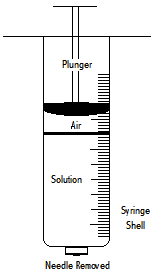
\includegraphics[scale=0.8]{img/syringe.png}
\caption{Measuring volume with a syringe}
\end{center}
\end{figure}

Hazards and Safety: Remove the needle from the syringe. Never use syringes with the needles. Never provide needles to the students.

\subsection*{Squirt Bottle}
Tools Required: Hammer and nail to make hole in lid
Materials Required: Empty bottle, biro casing, IV tubing, super glue.

\begin{figure}[h]
\begin{center}
\def\svgwidth{50pt}
\input{./img/squirt-bottle.pdf_tex}
\caption{Squirt Bottle}
\end{center}
\end{figure}

\subsection*{Test tube}
Tools Required: flame\\
Materials Required: 10 mL plastic syringe\\
Manufacturing Procedure: Remove the plunger from the syringe. Head the nozzle until it starts to melt and then press against a hard surface. If the resulting tube leaks water, heat and press again.
Hazards and Safety: Remove the needle from the syringe. Never use syringes with the needles. Never provide needles to the students.

\subsection*{Test tube holder}
Clothes pin, piece of paper.

\subsection*{Test tube rack}
Tools Required: knife or razor blade\\
Materials Required: cardboard\\
Manufacturing Procedure: Make two parallel folds in the cardboard to elevate the central section. Make "X" cuts in the central section. A test tube can be pushed through these cuts to hold it when not in use.

\begin{figure}[h]
\begin{center}
\def\svgwidth{150pt}
\input{./img/test-tube-rack.pdf_tex}
\caption{Test Tube Rack}
\end{center}
\end{figure}

\subsection*{Water Baths}
If using a kerosene or charcoal stove, this is just a heated pot (sufuria) of water. If using Motopoa, read the instructions in the section on Heat Sources.

%\section{Laboratory Safety}

\subsection{Laboratory Rules}

\subsection{First Aid}

[INSERT ACTIVITY HERE]

\section{Heat Sources}

Heat and flames are important for teaching chemistry. This section discusses low cost options for both heating solutions and higher temperature flames. This section also discusses safety specific to heating and fire. Finally, this section includes activities to teach students about luminous and non-luminous flames as well as basic fire fighting technique.

\subsection{Options for Heat Sources}

\subsubsection{Motopoa Burners}

These are the simplest stoves and the most practical for the chemistry laboratory. Motopoa is a heavy oil mixed with an organic alcohol. The fuel lights easily and burns hot, generally with a non-luminous (invisible) flame.

While there are commercial Motopoa stoves for cooking, a laboratory burner is only a small metal container. For small heating experiments - qualitative analysis, thermal decomposition, binary combination - the best container is the metal cap from a liquor bottle, e.g. Konyagi brand. Remove the plastic from the cap and fill it half way with Motopoa. Light the Motopoa with a match or gas lighter. No wick is required. The flame is difficult to see in bright light; carefully feel for heat to see if it has lit. To extinguish (put out) a Motopoa flame, blow on it like a candle.

Larger burners may also be constructed for heating water bathes, etc. Find an approximately 1 litre metal can and cut out the bottom and ventillation holes in the sides. Place this over a smaller can of Motopoa and rest a cooking pot on the top of the larger can.

\subsubsection{Kerosene Stoves}

Kerosene stoves may also be used for heating water bathes. Kerosene is less expensive than Motopoa but produces unpleasant smoke when burned and is more dangerous as a fuel because spills easily spread. The stoves are also more difficult to light and put out, and must be purchased rather than locally manufactured.

\subsubsection{Charcoal Stoves}

Charcoal stoves are useful when heat is required for a long time. Charcoal stoves take a long time to heat up. Charcoal burning properly should not produce smoke, though a stove with insufficient airflow may produce carbon monoxide.

\subsection{Types of Flames}
Many chemistry practicals involve the use of flame for heating, thus it is important for students to understand the different ways to produce flames in the laboratory. There are two kinds of flame: luminous and non-luminous. A luminous flame is one that produces a lot of light. The best flame in the chemistry lab is a non-luminous flame because it is hotter and does not produce soot. Unfortunately, in books the most common method given for producing the two types of flame is a bunsen burner. This activity is written to introduce students to different types of flames without the use of a bunsen burner. This activity is best done by students in small groups but the teacher should supervise the groups closely as they will be dealing with fires.
\subsubsection*{Learning Objectives}
\begin{itemize}
\item{To produce luminous and non-luminous flames from different fuel burners.}
\item{To demonstrate the combustion of various substances in air.}
\end{itemize}

\subsubsection*{Materials}
kerosene burner*, motopoa burner*, candle,  methylated spirit, kerosene, paper, motopoa, metal spoon, matches, metal jam-jar lid

\subsubsection*{Hazards and Safety}
\begin{itemize}
\item{This experiment involves open flames a bucket of water or sand should be available for fire fighting purposes.}
\end{itemize}

\subsubsection*{Activity Procedure}
\begin{enumerate}
\item{Light a kerosene burner and observe the flame. Adjust the heights of the wicks to change the appearance of the flame. Hold the metal spoon over the flame for a few seconds and then examine it for soot.}
\item{Put a small amount of methylated spirit into a soda bottle lid. Observe the flame. Hold the metal spoon over the flame for a few seconds and examine it for soot.}
\item{Light the motopoa burner. Observe the flame. Hold the metal spoon over the flame for a few seconds and examine it for soot.}
\item{Light the candle. Observe the flame. Hold the metal spoon over the flame for a few seconds and examine it for soot.}
\item{Put a small piece of paper into the metal lid and light it. Observe the flame. Hold the spoon over the flame for a few seconds and examine it for soot.}
\end{enumerate}

\subsubsection*{Results and Conclusion}
The kerosene produces a luminous flame. Adjusting the wick length can change the nature of the flame. When the wicks are very long you shold observe a bigger and brighter flame that is more likely to produce soot. If the metal cover is removed, the flame will be luminous and produce a lot smoke.
Spirit burns as a non-luminous flame that is colourless. The flame will be nearly invisible and will not produce soot.
Motopoa burns as a non-luminous flame. The flame will not produce soot.
A candle produces a luminous flame that deposits soot on the spoon.
A piece of paper produces a luminous flame that deposits soot on the spoon.
\subsubsection*{Discussion Questions}
\begin{enumerate}
\item{Which substances produced soot when burned?}
\item{Identify which substances produce luminous flames? Which substances produce non-luminous flames?}
\item{Which of the materials tested is best for heating in the chemistry laboaratory? Give reasons.}
\item{Which of the materials tested is worst for heating in the chemistry laboaratory? Give reasons.}
\end{enumerate}

\subsection{Fire Fighting}
Many chemistry activities involve the use of fire as a heat source. It is very important that students have an understanding of how to extinguish various fires in the laboratory. The most common sources of fire in the chemistry laboratory are kerosene, spirit, motopoa and paper/wood. The common available materials for extinguishing fires are water, sand and exhaled carbon dioxide. This activity give students the chance to explore and identify the best methods for extinguishing fires. This information will be very useful in case of an accident during later activities. This activity can be a useful demonstration but it is most effective if performed by students in small groups so they gain experience and knowledge on how to respond in case of a fire.
\subsubsection*{Learning Objectives}
\begin{itemize}
\item{To demonstrate the proper use of available materials in extinguishing various types of fire in the laboratory.}
\end{itemize}

\subsubsection*{Materials}
methylated spirit, motopoa*, candle, paper, sand, water, syringe, soda bottle tops, matches, glass jar, beaker

\subsubsection*{Hazards and Safety}
\begin{itemize}
\item{This experiment involves open flames a bucket of water or sand should be available for fire fighting purposes.}
\end{itemize}

\subsubsection*{Activity Procedure}
\begin{enumerate}
\item{Put a small amount of ethanol into a bottle cap and light it with a match. Pour water onto the flame.}
\item{Dry the cap and add a small amount of ethanol and light it again with a match. Put a handful of sand onto the flame.}
\item{Clean the cap and add a small amount of ethanol and light it again with a match. invert a glass jar over the flame and wait.}
\item{Put a small amount of kerosene into a bottle cap and light it with a match. Using a syringe, \textit{carefully} add a few drops of water near the base of the flame.}
\item{To the kerosene flame ad a handful of sand.}
\item{Clean the cap and add a small amount of kerosene and light it again with a match. Invert a glass jar over the flame and wait.}
\item{Fill a beaker with water.}
\item{Light a piece of paper on fire. Immediately dip it in the beaker of water.}
\end{enumerate}

\subsubsection*{Results and Conclusion}
A flame caused by burning ethanol is extinguished by the addition of water or sand. When the glass jar is inverted over the flame it will be deprived of oxygen and slowly go out. This is a useful demonstration because there a flame in a container, it can be extinguished by closing or covering the container.
A kerosene fire can NOT be extinguished by water. Because water is immiscible with kerosene, addition of water will only cause the fire to spread. Sand can be used to extinguish the kerosene flame.
Paper is easily extinguished by water.

\chapter{Fire}
Fire is used frequently in the chemistry laboratory. It is also used quite a bit in the home. Therefore, a good understanding of fire is very important.
The activities in this chapter give students the chance to investigate the factors necessary for combustion to occur and the products of combustion. Finally, this section gives an activity for students to investigate the product of combustion.

\subsection{Investigating the Requirements for Combustion}
Combustion is the rapid chemical combination of a substance with oxygen to produce heat and light. There are three things required for combustion to occur: fuel, oxygen and a high enough temperature (called the kindling temperature). This activity gives students the chance to observe what happens when the oxygen supply is cut off from a flame. It is a very simple and quick activity that is best done as a demonstration for the class.
\subsubsection*{Learning Objectives}
\begin{itemize}
\item{To identify the factors necessary for combustion to take place.}
\end{itemize}

\subsubsection*{Materials}
A candle, match box, a glass or metal cover and two beakers*.

\subsubsection*{Preparation Procedure}
\begin{enumerate}
\item{Cut the candle into two pieces about 5-7 cm long each and place them in each of the beakers.}
\end{enumerate}

\subsubsection*{Activity Procedure}
\begin{enumerate}
\item{Light the candles and leave them to burn for some time.}
\item{Cover the first beaker while the candle is still burning with a fire proof material (glass or metal) to prevent air from entering.}
\item{Leave the second beaker open so there is a continuous supply of air. Observe what happen.}
\end{enumerate}

\subsubsection*{Results and Conclusions}
In the first beaker, lack of oxygen extinguishes the candle flame after some time. In the second beaker the flame will continue to burn due to the constant supply of oxygen gas. 

\subsubsection*{Clean Up Procedure}
Collect all the used materials, cleaning and storing items that will be used later. No special waste disposal is required.

\subsubsection*{Discussion Question}
Explain what happened in the two beakers and why.


\subsection{Investigating the Products of Combustion}

Combustion is the rapid chemical combination of a substance with oxygen, producing heat and light. Most combustion activities involve burning compounds containing carbon and hydrogen. The carbon in the compound combines with oxygen to form carbon dioxide and the hydrogen combines with oxygen to form water. Therefore we expect carbon dioxide and water to be the products of most combustion activities.

The following activity is to demonstrate the production of carbon dioxide in one case of combustion: the burning of a candle. This activity requires about half an hour to show results, should it should be started at the beginning of the lesson and discussed near the end.

\subsubsection*{Learning Objectives}
\begin{itemize}
\item{To identify carbon dioxide as a products of combustion.}
\end{itemize}

\subsubsection*{Materials}
Candle, match box, plastic water bottle, lime water*, deflagrating spoon* or stiff wire.

\subsubsection*{Activity Procedure}
\begin{enumerate}
\item{Cut a 1.5 litre drinking water used bottle by its neck, as illustrated.}
\item{Add 20 - 30 mL of lime lime water to the cut bottle.}
\item{Mount abut 5 cm piece of wax candle on the deflagrating spoon. If no deflagrating spoon is available, attach the candle to a metal wire by twisting the end of the wire around the candle.}
\item{Light the candle and lower it into the lime water container so that the flame will sit above the surface of the lime water, as illustrated.}
\item{Observe the candle, which product(s) can you see?}
\item{Put your hand 5-10 cm above the candle, what can you feel?}
\item{Observe the lime water 5 minutes, 15 minutes, and 30 minutes after adding the candle. What change to you observe in the lime water?}
\end{enumerate}

\begin{figure}[h]
\begin{center}
\def\svgwidth{350pt}
\input{./img/combustion-products.pdf_tex}
\caption{Preparation of a Beaker}
\end{center}
\end{figure}

\subsubsection*{Results and Conclusions}
Light can easily be seen from a burning candle. Above the flame, soot may also be visible. Heat can be felt when the hand is placed above the flame. When the candle burns for some time the lime water turns milky, showing that there is production of carbon dioxide gas.

\subsubsection*{Clean Up Procedure}
Collect all the used materials, cleaning and storing items that will be used later. No special waste disposal is required.

\subsubsection*{Discussion Questions}
\begin{enumerate}
\item{What are the products of combustion?}
\item{Why does lime water turn milky when the candle burns?}
\item{What will happen to the lime water when the candle burns for more than 30 minutes in production of excess carbon dioxide?}
\end{enumerate}

\subsubsection*{Notes}
The products of combustion are light, heat energy, carbon dioxide gas and soot. Some fuels produce more soot or heat than other fuels. If time permits this fact could also be demonstrated by burning some different materials (outside) as a demonstration.

Note that the lime water must be very clear to notice the difference caused by the candle. It may be necessary to filter the lime water during the preparation.


%The others are split by chapter.
\chapter{The Nature of Matter and Physical Change}

Chemistry is the study of matter. All of the higher lessons depend on students' understanding of the basics of matter. Much of the study of chemistry is based on three simple postulates:
\begin{itemize}
\item{Matter is composed of extremely small particles called molecules.}
\item{Attraction forces cause these molecules to stick together.}
\item{Thermal energy keeps these particles in constant motion, sometimes shaking them apart from each other.}
\end{itemize}

%The rest of the study of chemistry is based on the structure of the atom, the manner in which electrons attract other atoms to form chemical bonds, and the nature of these bonds.

\section{Concept of Matter}

Everything we see is made up of extremely tiny particles called molecules. A molecule is the smallest unit of a substance that retains the chemical properties of the substance. Emphasis should be given to the extremely small nature of molecules: in 1 litre of water there are more than $$33,000,000,000,000,000,000,000,000,000$$ (`33 billion billion billion') molecules of water! Write this number on the board for students to think about.


\section{States of Matter}

Molecules are always in motion, although their movements are usually restricted by forces attraction to other molecules. The balance between thermal energy and intermolecular attraction determines the state of matter.
There are three states of matter: solid, liquid, and gas. A solid has fixed volume and fixed shape. A liquid has fixed volume but will take the shape of its container. A gas will take the volume and the shape of its container. A `vapour' is another word for gas often used for compounds that are normally liquid or solid at room temperature. For example, we might talk about `water vapour' or `zinc vapour,' but generally not `oxygen vapour.'


\subsection{Changes of State}
By changing the temperature of a substance, we can change the state it exists in. As a solid object is heated the molecules begin to shake faster and faster until they break free of the rigid solid substance and become a free-flowing liquid. This is called melting. A change of state is a physical change which involves a substance going from one state to another. \\

\begin{figure}[h!]
\begin{center}
\def\svgwidth{250pt}
\input{./img/triangle.pdf_tex}
\caption{Changes of State}
\end{center}
\end{figure}

Changes of state are something that students see in everyday life (a melting candle, drying clothes). This activity is good for getting students to think about these everyday changes in terms of the molecules which make up every substance. The activity demonstrates melting, solidifying, vaporization, and condensing. If enough candles are available, the students can do the first activity and make observations in small groups. Because of materials, time and safety it might be ideal to do the vaporization and condensing of water as a class demonstration and discussion.

\subsubsection*{Learning Objectives}
\begin{itemize}
\item{To describe the states of matter.}
\item{To demonstrate changes in state of various material.}
\end{itemize}

\subsubsection*{Materials}
candle, heating vessels*, water, condenser*, knife, heat source

\subsubsection*{Hazards and Safety}
\begin{itemize}
\item{Never heat a tightly sealed container.}
\end{itemize}

\subsubsection*{Preparation}
\begin{enumerate}
\item{Fill the condenser with cold water.}
\end{enumerate}

\subsubsection*{Activity Procedure}
\begin{enumerate}
\item{Take a candle and light it using a match box. Make observations about any changes observed.}
\item{Blow the candle out. Make observations about any changes.}
\item{Put about 20 mL of water in the heating vessel and heat for 5-10 minutes. Make observations.}
\item{Put about 50 mL in a heating vessel and connect with the condenser. Heat until a liquid is noticed at the other end of the condenser. Collect this liquid.}
\end{enumerate}

\subsubsection*{Results and Conclusion}
When the candle burns it changes from solid to liquid. When the candle cools the wax will harden, returning to solid state.
Boiling water is a change from a liquid to a vapour in gaseous state. Condensing water vapour changes it back from gas to liquid.

\subsubsection*{Clean Up Procedure}
\begin{enumerate}
\item{Collect all the used materials, cleaning and storing items that will be used later. No special waste disposal is required.}
\end{enumerate}

\subsubsection*{Discussion Questions}
\begin{enumerate}
\item{Explain what change of state is involved when burning candle wax and boiling water.}
\item{What happens when water is heated and passed through a condenser?}
\end{enumerate}

\section{Compounds and Mixtures}
When two substances are mixed together without making or breaking chemical bonds a mixture is formed. Mixtures can be separated by purely physical means. When two substances react such that chemical bonds are broken and new ones are made, the resulting substance is called a compound. This section deals with mixtures, where chemicals are mixed together but chemical reactions have not yet occurred.

\subsection{Solutions, Suspensions and Emulsions}
When a liquid is combined with another substance, three kinds of mixtures are possible: solution, suspension or emulsion. 
A \textit{solution} is a mixture where one component (solute) dissolves completely in the other (solvent) to form a transparent liquid. A \textit{suspension} is formed when a small pieces of solid are suspended or dispersed throughout a liquid without dissolving in it. The solute particles in the suspension remain visible.  An \textit{emulsion} is a fine dispersion of small droplets of one liquid in another in which it is not soluble or miscible. 
Solutions, suspensions and emulsions are something students encounter in every day life - salt water is a solution, river water is a suspension and milk is an emulsion.
This activity gives students a chance to make their own examples of each type of mixture and compare them side by side. This activity is best done by students in small groups so that each students gets a chance to make clear observations (it is hard to see the difference between a solution and a suspension from far away).

\subsubsection*{Learning Objectives}
\begin{itemize}
\item{To prepare examples of solution, suspension and emulsion.}
\item{To explain the properties of solutions, suspensions and emulsion.}
\end{itemize}

\subsubsection*{Materials}
Cooking oil, water, methylated spirit, test tubes*, beakers, plastic bottles with lids, copper (II) sulphate, clay soil.

\subsubsection*{Preparation}
\begin{enumerate}
\item{Grind the solid clay to make a fine powder.}
\end{enumerate}

\subsubsection*{Activity Procedure}
\begin{enumerate}
\item{Instruct students to mix equal volumes of cooking oil and water in a test tube and shake it vigorously.}
\item{Direct students to allow the solution in the test tube to settle. Have them record their observations.}
\item{Instruct students to add about a mL of methylated spirit to the test tube and again shake vigorously.}
\item{Students should again allow the test tube to settle and record their results. The mixture formed should be an emulsion.}
\item{Tell students to add a spoon of clay to a test tube of water and shake vigorously then set the test tube down and allow the solution to settle.}
\item{Direct students to add half of a spoonful of copper (II) sulphate to about 200 mL of water and shake vigorously until no more crystals are visible.}
\item{Instruct student to allow the mixture to sit for some minutes and record their observations.}
\end{enumerate}

\subsubsection*{Results and Conclusion}
In the first experiment oil and water clearly form two layers because they are immiscible liquids. Upon addition of methylated spirit and shaking, the two liquids form an emulsion. The emulsion is not transparent, you can not be seen in it.
The clay mixes with water to form suspension which after some time will settle to the bottom of the container. The suspension is not transparent and individual clay particles can clearly be seen.
The copper sulphate crystals dissolve in water completely to form a blue solution which does not settle no matter how long it is allowed to sit. The solution is transparent and individual particles can not be seen.

\subsubsection*{Clean Up Procedure}
\begin{enumerate}
\item{Collect the copper (II) sulphate solution, store in a labelled bottle and save for later use.}
\item{Collect all the used materials, cleaning and storing items that will be used later. No special waste disposal is required.}
\end{enumerate}

\subsubsection*{Discussion Questions}
\begin{enumerate}
\item{Did the oil and water separate after the addition of methylated spirit?}
\item{Can you see through the emulsion formed? Why?}
\item{Did the solid clay settle out of the clay mixture?}
\item{Can you see through the clay mixture?}
\end{enumerate}

\subsubsection*{Notes}
An emulsion can also be created by shaking a sodium hydroxide solution with cooking oil, however this is more dangerous than the procedure listed.

\section{Separation of Mixtures}

There are many methods of separating mixtures. Many are used in daily life. This topic is a good way to teach students that the chemistry they use in the classroom has application when they go home. This section presents different methods for separating mixtures and an activity to use for teaching each. Many of these methods will be important for more complicated experiments, so both students and teachers should be familiar with them.

\subsection{Decantation}
Decantation is an easy way to separate a suspension. Leave the suspension to settle, so the solid falls to the bottom of the container. Then, the liquid can be poured off the top. This method is applied in the home, for example, when rice is rinsed and the excess water is poured off. Students can perform this activity in a very short time; it is best combined with the filtration activity.


\subsection{Filtration}

Filtration is a more complicated but more effective method for separating a suspension. A suspension is filtered by passing it through a material with holes so small that only the liquid can pass through. The solid is left behind.

\subsection{Evaporation}

Evaporation is a simple method to separate solutions where one chemical is most more volatile than the other, for example a solution of salt in water.

\subsection{Separation of Mixtures: Decantation, Filtration and Evaporation}
This activity combines the principles of decantation, filtration and evaporation to produce a pure sample of salt from a mixture of salt, water, sand and stones. This activity is best done by student in small groups of 2-4.

\subsubsection*{Learning Objectives}
\begin{itemize}
\item{To separate  a mixture using the decantation, filtration, evaporation.}
\end{itemize}

\subsubsection*{Materials}
Water, sand, salt, small pebbles, beakers*, funnel*, clean cloth and a plastic bottle
\subsubsection*{Preparation}
\begin{enumerate}
\item{Make a mixture by combing water, salt, sand and pebbles an a plastic bottle. Close the lid and shake}
\end{enumerate}
\subsubsection*{Activity Procedure}
\begin{enumerate}
\item Shake the bottle well and observe the solution. Allow the bottle to sit for a few minutes so that the pebbles and some dirt settle to the bottom.
\item Pour the solution into a clean beaker, leaving the pebbles and dirt in the bottom of the bottle. You should now have a sample of water with some dirt particles.
\item Put the clean cloth in the filter and pour the dirty water into the filter. Make sure that all of the water passes through the cloth and not around the edges. Collect the water in a clean beaker. If dirt is still present in the water, filter it again through a fresh piece of cloth.
\item Put a small amount of this water into a clean beaker and leave it in the sun for a few hours. Make sure it is put in a place that is protected from wind so dirt does not enter. Once all of the water has evaporated collect the beaker and examine its contents.
\end{enumerate}

\subsubsection*{Results and Conclusion}
Decantation should separate the large pebbles and pieces of rocks. The filtration should remove all of the dirt particles and leave a clear salt water solution. After evaporation, salt crystals should remain in the beaker.

\subsubsection*{Clean Up Procedure}
\begin{enumerate}
\item{Collect all the used materials, cleaning and storing items that will be used later. No special waste disposal is required.}
\end{enumerate}

\subsubsection*{Discussion Questions}
\begin{enumerate}
\item{Give 3 examples each of decantation and filtration being used in daily life.}
\item{One problem with the method of evaporation is that the liquid is lost and cannot be collected again. Which method of separation could be used to separate salt water if pure water was the desired product.}
\end{enumerate}


\subsection{Construction of a Sand Filter}
In many villages there is no access to clean drinking water. People are forced to drink water that is unsafe or use a lot of fuel for boiling water. Many students are already aware of the process of boiling and filtering water to make it safe for drinking. On a larger scale, sand filters can be used to purify water for a group of people or even a village. When built properly on a large scale sand filters are even effective for removing micro-organisms which cause disease. In this activity students build small-scale sand filters and attempt to filter their own dirty water.  This activity is best done by students in small groups.

\textbf{NOTE}: The sand filters built in the laboratory are only an example, they are \textit{not} effective for removing bacteria from dirty water.
\subsubsection*{Learning Objectives}
\begin{itemize}
\item{To demonstrate the purification of water by using a sand filter.}
\end{itemize}

\subsubsection*{Materials}
Fine sand, coarse sand, small pebbles, large pebbles, charcoal, empty water bottle, beaker, screen material to act as a sieve, and dirty water.

\subsubsection*{Preparation}
\begin{enumerate}
\item{Use water to rinse all of the dirt off of the pebbles.}
\item{Put all of the sand in a sieve and shake to remove excess dirt. In the sieve, rinse the pebbles with water.}
\item{In a beaker, rinse the coarse sand with clean water and decant off the dirty water. Repeat until the water decanted is clear.}
\item{Cut the bottom off of a water bottle so that is it shaped like a funnel.}
\item{Invert the water bottle and fill the bottom with large pebbles, making sure that the bottom pebble is larger than the hole in the bottle so that it doest not fall out. Put a layer of smaller pebbles on top of the large pebbles.}
\item{Put the coarse sand particles on top of the pebbles, followed by charcoal and then small sand particles at the top (see diagram).}
((ILLUSTRATION))
\item{Run clean water through the filter until it comes out clear at the bottom.}
\end{enumerate}

\subsubsection*{Activity Procedure}
\begin{enumerate}
\item{Pour some dirty water into the top of the sand filter.}
\item{Collect the water in a clean beaker from the bottom of the filter.}
\end{enumerate}

\subsubsection*{Results and Conclusion}
When dirty water passes through sand particles, impurities are trapped and remain above. The smallest particles and some micro-organisms are stopped by the charcoal layer. Ideally, the water coming out of the bottom of the filter should be clear. 

\subsubsection*{Clean Up Procedure}
\begin{enumerate}
\item{Collect all the used materials, cleaning and storing items that will be used later. No special waste disposal is required.}
\end{enumerate}

\subsubsection*{Discussion Questions}
\begin{enumerate}
\item{How can you distinguish water before purification and water after purification?}
\item{List 3 substances which can make water impure.}
\item{Why is charcoal used in this process?}
\item{Why is water purification important?}
\end{enumerate}


\subsection{Separation of Mixtures: Simple Distillation}
Simple distillation is a more complicated method for separating solutions that allows the liquid to be collected. This method involves vaporizing the liquid, then condensing it by cooling the vapour, and collecting the resulting liquid.  The following activity involves a slightly complicates set-up so it is best done as a demonstration. If food colour is added to the water, even students in the back will be able to see the process.
\subsubsection*{Learning Objectives}
\begin{itemize}
\item{To be able to separate a solution by application of simple distillation}
\end{itemize}

\subsubsection*{Materials}
Condenser*, water, food colouring, heating vessel*, beaker, and heat source*.

\textbf{Notes}:

\begin{itemize}
\item{If food colouring powder is not available it is also possible to use a coloured compound like potassium permanganate or a salt. If a salt is used, it might be difficult to show that the distillate is salt free.}
\item{If a condenser is not available it is still possible to do this experiment. Connect a long delivery tube to a stopper on the heating vessel. The air temperature surrounding the tube will be cool enough to cause some water to condense which can then be collected in a beaker. If this method is used, a large amount of water will also be lost as steam.}
\end{itemize}

\subsubsection*{Preparation}
\begin{enumerate}
\item{Make a coloured solution by adding a small amount of colour to a sample of water.}
\item{Put cold water into the condenser.}
\end{enumerate}

\subsubsection*{Activity Procedure}
\begin{enumerate}
\item{Heat the container holding coloured water over the heat source for some time.}
\item{Collect any water out of the condenser and compare it to the original solution.}
\end{enumerate}

\subsubsection*{Results and Conclusion}
When the solution is heated, the water is vaporized while the coloured particles remain in solution. As the water vapour passes through the condenser tube is it cooled and condenses back to liquid form. The water will drip out of the end of the tube and will be pure, that is, containing no dissolved solutes. The final solution should contain no colour.

\subsubsection*{Clean Up Procedure}
\begin{enumerate}
\item{Collect all the used materials, cleaning and storing items that will be used later. No special waste disposal is required.}
\end{enumerate}

\subsubsection*{Discussion Questions}
\begin{enumerate}
\item{Why does the final solution appear different than the initial solution?}
\item{In what situation is simple distillation a better method of separation than evaporation?}

\end{enumerate}
\subsection{Separation of Mixtures: Sublimation}
Sublimation is the change of state from a solid straight to a gas. Because very few things sublimate at atmospheric pressure, so those that do can easily be separated form a mixture by heating. In this activity, students apply the method of sublimation to separate a mixture of iodine and sodium chloride. Iodine crystals sublimate when heated while sodium chloride does not. This activity is best done as a demonstration because iodine vapours are harmful if inhaled.
\subsubsection*{Learning Objectives}
\begin{itemize}
\item{To be able to separate a mixture containing iodine through sublimation.}
\end{itemize}

\subsubsection*{Materials}
Iodine crystals*, table salt, water, heating vessel (light bulb)*, and heat source*.
\subsubsection*{Hazards}
Iodine vapour is harmful if inhaled. Do this experiment in a well ventilated area.
\subsubsection*{Preparation}
\begin{enumerate}
\item{Make a mixture of iodine and salt by adding half a teaspoon of iodine crystals to a teaspoon of salt.}
\end{enumerate}

\subsubsection*{Activity Procedure}
\begin{enumerate}
\item{Heat the container holding the iodine/salt mixture gently over a heat source. Remove periodically from the flame and observe--iodine crystals should form on the top of the container. If no iodine crystals form, put a dish of cool water over the mouth of the heating vessel. Observe the bottom of the dish. }
\end{enumerate}

\subsubsection*{Results and Conclusion}
When the solution is heated, iodine sublimates to become iodine gas. When it comes into contact with the colder walls (or cover) of the container, it crystallizes out to form a solid.

\subsubsection*{Clean Up Procedure}
\begin{enumerate}
\item{Collect all the used materials, cleaning and storing items that will be used later. No special waste disposal is required.}
\end{enumerate}


\subsection{Separation of Mixtures: Chromatography}
Chromatography is the separation of a mixture by passing it in solution or suspension through a medium in which the components move at different rates. This method can be used to separate different coloured pigments in a coloured ink. Because each pigment has a different molecular shape, they can be dissolved in a solvent and separated. As the solvents moves through a medium (such as paper) the different molecules have different attraction to the paper and the solvent. Molecules with a higher attraction to the paper will move slower. After some time, the molecules will be separated, giving distinct bands of colour.

In this activity students are able to separate the different colour pigments present in the ink of a marker or pen. This activity should be done by students in small groups.
\subsubsection*{Learning Objectives}
\begin{itemize}

\item{To separate colours using paper chromatography.}

\end{itemize}

\subsubsection*{Materials}
Piece of white paper, cotton wick (utambi wa jiko), Petri dish*, colourless methylated spirit, small beaker* and one red marker or ball pen.

\subsubsection*{Preparation Procedure}
\begin{enumerate}
\item{Cut piece of paper to a size a little bigger than the top of the beaker. Put a small hole in the center of it.}
\item{Prepare a wick that is long enough to reach to the bottom of the beaker.}
\end{enumerate}

\subsubsection*{Activity Procedure}
\begin{enumerate}
\item{Pour the colourless spirit into the beaker.}
\item{Make a hole in the center of the piece of paper you have prepared and insert the thread through the hole. ((ILLUSTRATION NEEDED)) }
\item{Using a red marker/ball pen draw a circle around the hole and put the piece of paper on the beaker containing methylated spirit and make sure the end of the wick is immersed in the liquid.}
\item{Leave it to sit until the spirit has caused separation of the colours (this should be about 10 minutes).}
\item{Repeat the experiment using different markers or pens.}
\end{enumerate}

\subsubsection*{Results and Conclusion}
Methylated spirit acts as a solvent. The solvent climbs up the wick and then spreads across the paper.  When the solvent reaches the ink, the different pigments dissolve and move at different speeds and thus are separated. The colours observed for a red marker might be yellow, pink and purple.

\subsubsection*{Clean Up Procedure}
\begin{enumerate}
\item{Collect all the used materials, cleaning and storing items that will be used later. No special waste disposal is required.}
\end{enumerate}

\subsubsection*{Discussion Questions}
\begin{enumerate}
\item{Explain the use of the wick, methylated spirit and marker pen to this experiment.}
\item{How many colors are there on the piece of paper at the end of the experiment.}
\end{enumerate}


\subsection{Separation of Mixtures: Layer Separation}
Layer separation is a method of separation used to separate two liquids that are immiscible. Immiscible means that the liquids are mutually insoluble and thus form two distinct layers when mixed. The following activity give students a chance to separate a mixture of kerosene. The activity is very short and can be done in combination with another separation activity in a single class period.

\subsubsection*{Learning Objectives}
\begin{itemize}
\item{To separate two immiscible liquids using layer separation.}
\end{itemize}

\subsubsection*{Materials}
Kerosene, water, 2 plastic 1 litre water bottles, IV set, super glue, cello tape

\subsubsection*{Preparation}
\begin{enumerate}
\item{Construct a separatory funnel in the following way}
\begin{enumerate}
\item{Cut both water bottles just below the line of the label}
\item{Connect the two bottles together as shown in figure \ref{fig:sep-funnel} using super glue, making sure the seal is air tight. Wrap}
\item{In the lid of one bottle, poke a hole using a hammer and a nail. Insert the biro casing and super glue around the edges to create a water-tight seal.}
\item{Cut the infusion tube such that only two cm of the tube extend from the iv clip.}
\item{Fit the IV tubing over the biro casing, making sure the seal is water-tight}
\end{enumerate}
\end{enumerate}

\begin{figure}[h]
\begin{center}
\def\svgwidth{250pt}
\input{./img/separating-funnel_materials.pdf_tex}
\caption{Materials for Constructing a Separatory Funnel}
\label{fig:separating-funnel_materials}
\end{center}
\end{figure}

\begin{figure}[h]
\begin{center}
\def\svgwidth{50pt}
\input{./img/separating-funnel.pdf_tex}
\caption{Separatory Funnel}
\label{fig:sep-funnel}
\end{center}
\end{figure}

\subsubsection*{Activity Procedure}
\begin{enumerate}
\item{Measure approximately equal volume of water and kerosene using the small beaker and pour them in the separating funnel and shake them well.}
\item{Leave the mixture for some time to settle and run off the lower layer.}
\end{enumerate}

\subsubsection*{Results and Conclusion}
When water and kerosene are mixed and left to settle the two liquids form two immiscible layers. Kerosene forms the upper layer while water forms the lower layer because water is denser than kerosene. Water can be slowly drained from the separatory funnel and collected in a clean beaker.

\subsubsection*{Clean Up Procedure}
\begin{enumerate}
\item{Collect all the used materials, cleaning and storing items that will be used later. Kerosene should not be disposed. Put it in a well-labelled bottle and store for later use.}
\end{enumerate}

\subsubsection*{Discussion Questions}
\begin{enumerate}
\item{What are immiscible liquids?}
\item{In a kerosene/water mixture, which liquid is on top? Why?}
\end{enumerate}

\subsection{Separation of Mixtures: Solvent Extraction}

Solvent extraction is a method of separation used to separate a solute from its solvent by shaking it with a second immiscible liquid that is better at dissolving the solute. For example, iodine is much more soluble in organic solvents than in water. Iodine can be removed from a water solution by shaking it with an organic solvent (like kerosene) and then using layer separation to separate the two liquids.
The following activity give students a chance to extract iodine from a water based solution by using a sample of kerosene. The activity is best done my students in small groups.

\subsubsection*{Learning Objectives}
\begin{itemize}
\item{To demonstrate the principle of solvent extraction.}
\end{itemize}

\subsubsection*{Materials}
Kerosene, water, iodine tincture, test tubes*, beakers and stopper.

\subsubsection*{Preparation}
\begin{enumerate}
\item{Make an iodine solution by dissolving one part iodine for five parts water.}
\end{enumerate}

\subsubsection*{Activity Procedure}
\begin{enumerate}
\item{Put about 5 mL of the iodine solution in the test tube. Observe the colour.}
\item{Add about 2.5 mL of kerosene, cover with a stopper and shake vigorously for about a minute.}
\item{Leave the mixture for some time and observe any colour changes from the initial liquids. Allow the mixture to settle and decant off the upper layer of kerosene into a clean beaker.}
\item{Add another 2.5 mL of kerosene to the remaining water and shake again. Again observe the colours present. Decant off the top layer of kerosene into the kerosene beaker.}
\end{enumerate}

\subsubsection*{Results and Conclusion}
When the iodine solution is shaken with kerosene, the iodine is extracted into the kerosene layer. This is because iodine is a non-polar solute so it is more soluble in the non-polar solvent (see the following activity). The kerosene will turn to a deep red colour upon shaking. 

\subsubsection*{Clean Up Procedure}
\begin{enumerate}
\item{Collect all of the used kerosene and mix with a solution of vitamin C (ascorbic acid). This will remove the iodine from solution. Repeat until the kerosene has lost the deep red colour. If no Vitamin C is present, do not pour the kerosene down the drain or in the sink, rather set it out away from people and allow to evaporated. The ascorbic acid can be safely disposed of down the sink.}
\item{Collect all the used materials, cleaning and storing items that will be used later. Kerosene should not be disposed. Put it in a well-labelled bottle and store for later use.}
\end{enumerate}

\subsubsection*{Discussion Questions}
\begin{enumerate}
\item{What did you observe when you mixed? Why did this happen?}
\item{How is this process used in industry?}
\item{Why is supu with hot peppers more spicy than hot peppers in water?}
\end{enumerate}




\section{Solubility}

\subsection{Comparing Solubility}

\subsubsection*{Learning Objectives}
\begin{itemize}
\item{To compare the solubility of different substances in water and organic solvents.}
\end{itemize}

\subsubsection*{Materials}
Sugar, kerosene, table salt, steel wool, iodine crystals*, potassium permanganate crystals*, water, beaker*, test tube*.

\subsubsection*{Preparation Procedure}
\begin{enumerate}
\item{Break the steel wool into small piece.}
\end{enumerate}

\subsubsection*{Activity Procedure}
\begin{enumerate}
\item{In a test tube, combine about 1 mL of kerosene and 1 mL of water. Write down your observations.}
\item{Put half a spoonful of sugar into about 10 mL of kerosene in beaker labelled kerosene. Make observations.}
\item{Put half a spoonful of sugar into about 10 mL of water in a beaker labelled water. Compare the solubility of sugar in kerosene and water.}
\item{Dump out the sugar water solution and decant the kerosene into a beaker for later use.}
\item{Repeat the test using salt and steel wool, each time dumping the water solution and saving the kerosene.}
\item{Repeat with iodine and potassium permanganate, this time using only a few crystals. Record observations.}
\end{enumerate}

\subsubsection*{Results and Conclusion}
Sugar and salt dissolve in water but not kerosene. Iron does not dissolve in either solvent. Potassium permanganate dissolves in water to make a deep purple solution but does not dissolve in kerosene. Iodine dissolves only a small amount in water but in kerosene dissolves to make a deep red solution.

\subsubsection*{Clean Up Procedure}
\begin{enumerate}
\item{Kerosene can be decanted to remove any solid and stored for later use. Kerosene containing iodide should be left in an open container away from people until it has completely evaporated.}
\item{Potassium permanganate can be stored in a container for later use. If it is disposed, it should be reduced with vitamin c (ascorbic acid) prior to being dumped in the drain.}
\end{enumerate}

\subsubsection*{Discussion Questions}
\begin{enumerate}
\item{What is the solubility of sugar, iron and salt in water and organic solvent?}
\item{Compare the solubilities of potassium permanganate and iodine in water and kerosene.}
\end{enumerate}

\subsubsection*{Notes}
Water is a polar substance. Kerosene is non-polar. In solubility the general rule is "like dissolves like". Polar substances like water dissolve polar or ionic solutes like salt, sugar and potassium permanganate. Non-polar solvents like kerosene dissolve non-polar substances like iodine. Most organic substances are non-polar hence can not dissolve in water. Kerosene does not dissolve water and water does not dissolve kerosene, hence they form two layers when mixed.

From \chapter{Chemical Change and Chemical Reactions}


\section{Physical and Chemical Changes}

Changes in state are an example of a physical change. A physical change is a change that only involves rearranging molecules. Chemists also study chemical changes, in which chemical bonds are broken and remade, and molecules change from one kind to another. The following activity may be used with students to illustrate the difference between physical and chemical changes.

\subsection{Physical and Chemical Change}

\subsubsection*{Learning Objectives}
\begin{itemize}
\item{To demonstrate physical and chemical changes of matter experimentally.}
\end{itemize}


\subsubsection*{Materials}
A piece of paper, sugar, spoon, bar magnet, two iron nails, steel wool, kerosene stove and match box.

\subsubsection*{Activity Procedure}
\begin{enumerate}
\item{Take a piece of paper and light it on fire using a match box. Have students record their observations.}
\item{Take a small amount of sugar into the spoon and heat until a clear chemical change is observed. Have students record their observations.}
\item{Take a bar magnet and rub one nail in one direction only.}
\item{ Place the second (un-magnetized) nail hear the iron fillings . Repeat with the nail that has been rubbed with a magnet.}
\item{Take the magnetized nail and rub it again in the opposite direction and place in iron fillings observe what will happen.}
\end{enumerate}

\subsubsection*{Results and Conclusion}
Burning paper and burning sugar are examples of chemical changes. These means that chemical bonds are broken and remade and new products are formed. But when the nail is rubbed with the bar magnet no chemical bonds are broken or made. The nail becomes magnetized and thus attracts the iron fillings. This is an example of a physical change.

\subsubsection*{Clean Up Procedure}
\begin{enumerate}
\item{Collect all the used materials, cleaning and storing items that will be used later. No special waste disposal is required.}
\end{enumerate}

\subsubsection*{Discussion Questions}
\begin{enumerate}
\item{Explain the changes in the paper and sugar. Name the type of change.}
\item{Explain the process of rubbing a nail with a bar magnet and what happen when it was rerubbed?}
\item{Why did the two nail behave differently? Name the change that happened in the rubbed nail.}
\end{enumerate}


\section{ Chemical Reactions}
Chemical reactions are chemical changes - chemical bonds are broken and remade. This section includes examples of three common types of reactions - thermal decomposition, binary combination, and precipitation - and activities to guide students to better understand these reactions. There is also a discussion of solubility and another activity to do with students.
\subsection{Precipitation Reaction}
A precipitate reaction is the formation of an insoluble salt by mixing solutions which contain its two components. These reactions are great for teaching students because of the speed and dramatic changes involved. The principles or precipitation are used in many future practicals-including identifying unknowns in qualitative analysis-so this activity is a good introductions to the principles. This activity is best done individually by students or in small groups of 2-3. 

\subsubsection*{Learning Objectives}
\begin{itemize}
\item{To explain the meaning of a precipitation reaction.}
\item{To write chemical equations for the precipitation of insoluble salt.}
\end{itemize}

\subsubsection*{Materials}
copper sulphate*, soda ash (sodium carbonate)*, beakers*, funnel* and filter paper* (or cloth).

\subsubsection*{Preparation}
\begin{enumerate}
\item{Make a solution of copper sulphate by dissolving about 1 spoonful in 500 mL of water.}
\item{Make a solution of sodium carbonate by dissolving about 1 spoonful in 500 mL of water.}
\end{enumerate}

\subsubsection*{Activity Procedure}
\begin{enumerate}
\item{Take one empty beaker and add about 10 mL of copper sulphate solution.}
\item{To the same beaker add about 10 mL of sodium carbonate solution.}
\item{Filter the mixture and save the insoluble salt.}

\end{enumerate}

\subsubsection*{Results and Conclusion}
When copper sulphate solution is mixed with sodium carbonate a precipitate will form. Copper carbonate is a blue precipitate. This reaction is useful for preparing insoluble salts.
The chemical reactions are 
$$ \ce{CuSO4} _{(aq)} + \ce{Na2CO3}_{(aq)}\longrightarrow \ce{CuCO3}_{(s)} \ce{Na2SO4}_{(aq)} $$

\subsubsection*{Clean Up Procedure}
\begin{enumerate}
\item{Collect all the copper carbonate produced and save for the following pracical (thermal decomposition).}
\item{Collect all the used materials, cleaning and storing items that will be used later. No special waste disposal is required.}
\end{enumerate}

\subsubsection*{Discussion Questions}
\begin{enumerate}
\item{What precipitate is formed in this reaction?}
\item{Write a balanced chemical equation for this reaction.}
\end{enumerate}

\subsubsection*{Notes}
The precipitated copper carbonate should be saved for the following experiment (thermal decomposition).

\subsection{Thermal Decomposition}

Thermal decomposition is when a compound breaks down when heated. Many compounds decompse when heated. Generally there are two products of thermal decomposition -- a gas that leaves the sample and a residue that stays behind. 

\subsubsection*{Learning Objectives}
\begin{itemize}
\item{To explain the meaning of thermal decomposition.}
\item{To observe thermal decomposition of both a salt and an organic compound.}
\item{To write chemical equations for the thermal decomposition a salt.}
\end{itemize}

\subsubsection*{Materials}
copper carbonate (from the above experiment), citric acid*, metal spoon, heat source

\subsubsection*{Preparation}
\begin{enumerate}
\item{Dry copper carbonate from the precipitation reaction experiment by leaving it in an open container.}
\end{enumerate}

\subsubsection*{Activity Procedure}
\begin{enumerate}
\item{Place a small amount of copper carbonate in a metal spoon.}
\item{Heat the sample until only a black residue remains.}
\item{Place a small amount of citric acid in a metal spoon.}
\item{Heat the sample until only a black residue remains.}

\end{enumerate}

\subsubsection*{Results and Conclusion}
When copper carbonate is heated, it decomposes to release carbon dioxide. The black reside can be found by subtracting carbon dioxide from the formula for copper carbonate:

$$ \ce{CuCO3} _{(s)} \longrightarrow \ce{CO2}_{(g)} + \ce{CuO}_{(s)} $$

When citric acid is heated, it decomposes twice. First, bubbles of carbon dioxide are released. Then, citric acid further decomposes to release water vapor. The black residue at the end of the experiment is solid carbon.

\subsubsection*{Clean Up Procedure}
\begin{enumerate}
\item{Allow spoons to cool before cleaning. Note that hot spoons can burn wood tables.}
\item{Scrap off the residues with another metal spoon and then steel wool. The copper oxide may be saved for future experiments. Neither copper oxide nor solid carbon require special disposal; the solid waste may be put in a pit latine or trash pit.}
\end{enumerate}

\subsubsection*{Discussion Questions}
\begin{enumerate}
\item{What gas is released in the decomposition of copper carbonate?}
\item{Write a balanced chemical equation for this reaction.}
\end{enumerate}

\subsubsection*{Notes}
Thermal decomposition of organic compounds is also called pyrolysis. This is the same process used to make charcoal from plant material.

\subsection{Binary Combination}
Binary combination is the kind of chemical reaction where two elements come together to form a compound. The elements alone are often quite different from the compounds they make up. Iron is a hard, magnetic, silver metal and sulphur is a yellow powder. When heated, the two combine to form iron (II) Sulphide FeS which is a black, insoluble compound. 

This activity gives students a chance to observe a binary combination reaction by heating sulphur and iron together. The students will investigate the properties of the elements before the reaction as well as the final product. Because this activity might lead to the production of a gas that could be harmful in large amounts, it is best as a teacher demonstration.

\subsubsection*{Learning Objectives}
\begin{itemize}
\item{To demonstrate a binary combination reaction.}
\item{To write a balanced equation for the binary combination of iron and sulphur.}
\end{itemize}

\subsubsection*{Materials}
Sulphur*, steel wool, source of heat*, tea spoon, heating vessel*, bar magnet and aluminium plate.

\subsubsection*{Hazards and Safety}
\begin{itemize}
\item{This reaction produces sulphur dioxide, a poisonous gas. Perform this reaction outside or in a well-ventilated room and stand upwind.}
\item{This experiment involves open flames a bucket of water or sand should be available for fire fighting purposes.}
\end{itemize}

\subsubsection*{Preparation}
\begin{enumerate}
\item{Grind the steel wool using a spoon on a hard surface so that fine particles are obtained.}
\end{enumerate}

\subsubsection*{Activity Procedure}
\begin{enumerate}
\item{Put half a teaspoon of iron particles in a beaker and add the same amount of sulphur powder. Mix them well.}
\item{Put a bar magnet into the mixture and observe the results.}
\item{Put some iron fillings in the heating vessel, add twice as much sulphur powder to it and mix them well. Heat the mixture until the sulphur powder is gone.}
\item{Again use a bar magnet to try to separate the two components physically from the mixture and record the results.}
\item{To another heating vessel put few iron fillings, add sulphur powder to it and mix them. Heat the mixture strongly for an extended time.}
\item{Use a a bar magnet and to try separate the two components physically from the mixture and record the results. If nothing is observed on the bar magnet, continue heating and try again.}
\end{enumerate}

\subsubsection*{Results and Conclusion}
The mixture of sulphur and iron before heating can easily be separated by physical means because iron has magnetic properties while sulphur does not. When the second mixture is heated, the iron and sulphur combine to form iron (II) sulphide. Because the sulphur and iron are chemically bound together, they cannot be separated by physical means. In the third trial the iron sulphide is heated extensively, liberating the sulphur as sulphur dioxide. This leaves iron metal behind (or an iron oxide) which can be picked up using a magnet.

\subsubsection*{Clean Up Procedure}
\begin{enumerate}
\item{Collect all the used materials, cleaning and storing items that will be used later. No special waste disposal is required. Solid waste should not be put in the drain.}
\end{enumerate}

\subsubsection*{Discussion Questions}
\begin{enumerate}
\item{What do you understand by the term binary combination?}
\item{Write the equation for the binary combination of Iron and sulphur.}
\item{Why was there no effect of the bar magnet in mixture 2?}
\end{enumerate}

\subsection{Rusting}

Rusting is a chemical reaction similar to combustion which was seen in the first chapter. Chemically rusting is very similar to combustion. Both are examples of a materials undergoing destructive oxidation through reaction with oxygen gas. Iron rusts by reacting with oxygen and water to form a hydrated iron oxide called rust.

This activity is useful for showing students the conditions required for rusting - metal, oxygen (air), and water. After students learn about the requirements of rusting, they can participate in a discussion about how to prevent rusting. This activity should be performed by students working in small groups. The experiment should be started in one period and discussed in the next as at least 24 hours are required for results.
\subsubsection*{Objectives}
\begin{itemize}
\item{To demonstrate the conditions necessary for rusting}
\end{itemize}

\subsubsection*{Materials}
Oil, water, sealed syringes, syringe plungers, iron (non-galvanized) nails, iron wool* and paint.

\subsubsection*{Activity Steps}
\begin{enumerate}
\item{Label 6 sealed syringes with the numbers 1-6}
\item{Place a nail in syringe 1 and fill with water. Leave open to air. This is the control.}
\item{Place a nail in syringe 2 and fill with water. Place the plunger back to seal the syringe to prevent oxygen from entering the shell.}
\item{Place a nail in syringe 3 and cover with oil. Leave open to air.}
\item{Place a nail in syringe 4 and cover with oil. Replace plunger to seal the syringe.}
\item{Place a nail in syringe 5 cover with water. Make an oil layer with a thickness of at least 2 cm.}
\item{Take a nail and paint the nail to cover the metal completely. Now place in syringe 6 and fill with water.}
\begin{figure}[h]
\begin{center}
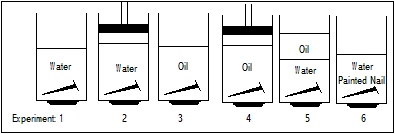
\includegraphics[scale=0.75]{../img/rust-prevention.png}
\caption{Rust Prevention}
\end{center}
\end{figure}


\end{enumerate}


\subsubsection*{Results and Conclusion}  
Syringe 1 is the control experiment. This will be the normal rusting of the iron nail. Syringe 2 now prevents any oxygen from participating in the rusting reaction. This nail should have little or no rust. Syring 3 allows oxygen to encounter the oil for rusting; however, there is no water since it is filled with oil. In addition, oxygen migrates through oil very poorly that also limits the available oxygen for rusting on the surface of the nail. There should be little or no rusting on the nail. Syringe 4 has no oxygen or water available for rusting. This nail should have no rusting. Experiment 5 allows water available to react, but now there is an oil layer. This oil layer prevents oxygen from entering the water layer and rusting the iron nail. This nail should have little or no rust. Syring 6 is much like the control, but since the nail is painted, there is no iron available to react since it is protected by the paint. In each of these experiments, the availability of the iron, oxygen, and water change and the effects of the lack of availability of each component slow down or even prevent the rusting reaction.
\subsubsection*{Clean Up Procedure}
\begin{enumerate}
\item{Collect all the used materials, cleaning and storing items that will be used later. No special waste disposal is required.}
\end{enumerate}
\subsubsection*{Discussion questions}
\begin{enumerate}
\item{Which nail had the most rust at the end? Which nail had the least?}
\item{What was the purpose of oil in this experiment? What was the function of the plunger?}
\item{Why are ships painted even on surfaces that cannot be seen?}
\end{enumerate}
\chapter{Water}

Water is fundamental to life. It is also essential in the chemistry laboratory. This section includes a series of activities to teach students about water - how to test for it, how to purify it, and much about hard and soft water.

\subsection{Test for Water}

\subsubsection*{Learning Objectives}
\begin{itemize}
\item{To understand the meaning of the words `hydrated' and `anhydrous.'}
\item{To test for the presence of water.}
\end{itemize}

\subsubsection*{Background Information}
Copper (II) sulphate exists in two forms: hydrated (with water) and anhydrous (without water). Hydrated copper (II) sulphate is blue while anhydrous copper (II) sulphate is white. Thus, white copper sulphate can be used as a test for water.

\subsubsection*{Materials}
Heat source*, copper (II) sulphate*, water, metal spoon

\subsubsection*{Activity Procedure}
\begin{enumerate}
\item{Instruct students to place a very small amount of blue copper (II) sulphate in a metal spoon.}
\item{Supervise students heating the spoon gently over a heat source. Students will stop heating when the crystals have changed from blue to white.}
\item{Instruct students to add a few drops of water to the white crystals. Students will observe and record any colour change.}
\end{enumerate}

\subsubsection*{Results and Conclusion}
On heating blue hydrated copper (II) sulphate, the colour changes from blue (CuSO4-5H2O) to white (CuSO4). On addition of a few drops of water CuSO4 returns to its original hydrated state (blue), i.e. copper sulphate pentahydrated.

\subsubsection*{Clean Up Procedure}
\begin{enumerate}
\item{Copper (II) sulphate crystals can be left in the air to dry the excess water and then used again in future experiments.}
\item{Collect all the used material, cleaning and storing items that will be used again later. No special waste disposal is required.}
\end{enumerate}

\subsubsection*{Discussion Questions}
\begin{enumerate}
\item{Explain what happens to the blue copper (II) sulphate when it is heated. What happened when water was added.}
\item{Write a balanced chemical equation for this reaction.}
\item{When anhydrous copper (II) sulphate is allowed to sit out for 30 minutes its colour changes from white to light blue. Explain why this happens.}
\end{enumerate}

\subsubsection*{Notes}

\subsection{Water Purification}

Natural water may contain harmful organisms and substances. Water purification is necessary before drinking in order to removed harmful micro-organisms and dirt particles. Water treatment is the process of making water safe and usable for either domestic, industrial or medical purpose. This activity allows students to practice proper water treatment.



\subsubsection*{Objectives}
\begin{itemize}
\item{To demonstrate proper treatment of drinking water.}
\end{itemize}

\subsubsection*{Materials}
clean piece of white cloth, boiling vessel (sufuria), heat source, impure water, bucket

\subsubsection*{Activity Procedure}
\begin{enumerate}
\item{Make the source of heat by lighting the stove.}
\item{Heat the water to boiling. Allow water to boil for 5 minutes.}
\item{Allow water to cool.}
\item{Use the clean white cloth to filter the water into a clean bucket. Water is now safe for drinking.}
\end{enumerate}

\subsubsection*{Results and Conclusion}
The act of boiling water at the boiling point (100 C) kills the germs and bacteria which may cause disease. Filtration with a piece of clean white cloth removes any solid impurities. The filtrate obtained is drinkable water.

\subsubsection*{Discussion Questions}
\begin{enumerate}
\item{Define the following terms (a) water treatment (b) water purification.}
\item{It is advised to let water boil for at least 5 minutes. Why?}
\item{Explain how the filtered water is different from the original water.}
\end{enumerate}

\subsubsection*{Notes}
Instead of a cloth, it is possible to use chemical purifiers for filtration such as "water guard" or "aqua guard".

\subsection{Differences between Soft Water and Hard Water}

The names soft water and hard water were developed before people understood chemistry. Even today the average person is familiar with the difference between water from place to place. In some places it is easy to use soap - it forms a soft lather easily and cleans hands and clothes effectively. In these places the water is called soft water. In other places, it is hard to use soap - much effort is required to get the lather required for cleaning. In these places the water is said to be hard water.

Now we know what causes some water to be hard water and other water to be soft water. Hard water contains dissolved magnesium or calcium ions. Soft water does not. While we cannot feel the difference between plain soft water and plain hard water, the difference is clear when using soap. Dissolved magnesium and calcium ions bind to the soap, forming a `scum' that is not effective for cleaning. Only with much soap can a useful lather be formed.

The following activity is useful for students to experience the difference between soft water and hard water. Students should perform this activity in small groups.

\subsubsection*{Objectives}
\begin{itemize}
\item{To differentiate between soft water and hard water.}
\end{itemize}

\subsubsection*{Materials}
Soft water (rain/distilled water), Gypsum powder*, epsom salt*, table salt, beakers*, sponge, and a bar of soap

\subsubsection*{Preparation}
\begin{enumerate}
\item{Label 5 beakers: CaSO4 solution, MgSO4 solution, NaCl solution, MgSO4 + CaSO4 solution and soft water.}
\end{enumerate}

\subsubsection*{Activity Procedure}
\begin{enumerate}
\item{Dip a sponge and soap into one solution after another while rubbing them together for several seconds.}
\item{Record the result from each beaker.}
\end{enumerate}

\subsubsection*{Results and Conclusion}
The three beakers labelled CaSO4 solution, MgSO4 solution and CaSO4 + MgSO4 solution all form soap scum, while the other two beakers containing soft water and NaCl solution easily formed a lather with soap.

\subsubsection*{Clean Up}
\begin{enumerate}
\item{Collect all the used materials, cleaning and storing items that will be used later. No special waste disposal is required.}
\end{enumerate}

\subsubsection*{Discussion Questions}
\begin{enumerate}
\item{What causes hardness of water?}
\item{How can you differentiate hard water from soft water?}
\end{enumerate}

\subsubsection*{Notes}
Permanent hardness of water is caused by the presence of Ca+2 and Mg+2 ions in solution. The two ions react with soap to form insoluble substance called scum. The formation of scum destroys the soap and prevents the formation of lather. Ca+2 and Mg+2 ions present in solution and destroys the soap as follows;
CaSO4(aq) + 2NaSt(aq)...... CaSt(aq) + Na2SO4.
MgSO4(aq) + 2NaSt(aq) ...... MgSt(aq) + Na2SO4.
(St represents stearate in these chemical equations.)

\subsection{Temporary Hard Water}

There are two kinds of hard water: temporary hard water and permanent hard water. A long time ago, people thought that only temporary hard water could be treated, whereas permanent hard water would always be hard. Now we know how to treat both kinds of hard water.

Temporary hard water has hydrogen carbonate anions. When temporary hard water is boiled, the hydrogen carbonate decomposes to form carbonate. Neither magnesium carbonate nor calcuim carbonate is soluble in water, so these salts precipitate. Therefore temporary hard water can be boiled to produce soft water.

The following activity is useful for students to observe the treatment of temporary hard water by boiling. Students should perform this activity in small groups, one for each available heat source.

\subsubsection*{Objectives}
\begin{itemize}
\item{To treat hard water by heating.}
\end{itemize}

\subsubsection*{Materials}
beakers*, heating vessel*, magnesium sulphate*, sodium hydrogen carbonate*, kerosene stove, match box, soft water (rain/distilled water), filter paper*, funnel* and sodium carbonate*.

\subsubsection*{Hazards and Safety}
\begin{itemize}
\item{((FIRE))}
\end{itemize}

\subsubsection*{Preparation}
\begin{enumerate}
\item{Make an open bulb and use it as heating vessel.}
\end{enumerate}

\subsubsection*{Activity Procedure}
\begin{enumerate}
\item{In a beaker labeled hard water put one spoon full of magnesium sulphate salt followed by two spoon fulls of sodium hydrogen carbonate and water up to height of 3-4 cm and stir well to mix.}
\item{In a second beaker add about 2-3 cm height of water and add two spoon fulls of washing soda and stir well to dissolve.}
\item{Put soft water in the third beaker.}
\item{Take a small amount (about 5-10 mL) of hard water and boil until no more precipitate is formed. Remove from heat and let it cool.}
\item{Fold the filter paper once in the middle, then repeat again so the second fold makes it fit in the funnel for the filtration.}
\item{Filter the boiled solution into a beaker labeled filtrate.}
\item{Put a few drops of sodium carbonate into soft water, hard water and filtrate. Note the changes.}
\end{enumerate}

\subsubsection*{Results and Conclusion}
Magnesium sulphate mixes with sodium hydrogen carbonate solution to produce temporary hard water which is magnesium hydrogen carbonate. Boiling temporary hard water causes precipitation of magnesium carbonate which is the way of removing the magnesium ions which are the ones causing hard water. This type of hardness can also be removed by precipitation method by the addition of washing soda. When the washing soda was added to hard water there was a precipitate of magnesium carbonate.

\subsubsection*{Clean Up Procedure}
\begin{enumerate}
\item{Collect all the used materials, cleaning and storing items that will be used later. No special waste disposal is required.}
\end{enumerate}

\subsubsection*{Discussion Questions}
\begin{enumerate}
\item{Define temporary hardness of water.}
\item{Why were magnesium sulphate and sodium hydrogen carbonate mixed? Write the chemical formulae of the resulting solution.}
\item{What is the precipitate formed during boiling?}
\item{Describe why there was precipitate in only one beaker.}
\item{What are other ways of removing hardness of water?}
\end{enumerate}

\subsubsection*{Notes}
Temporary hard water is often described as containing calcium hydrogen carbonate and magnesium hydrogen carbonate. This is a source of confusion. Temporary hard water indeed contains calcium/magnesium ions as well as hydrogen carbonate ions and thus can correctly be called a solution of calcium hydrogen carbonate (or magnesium hydrogen carbonate). Note, however, that neither calcium hydrogen carbonate nor magnesium hydrogen carbonate exists as a solid chemical. Thus the preparation of temporary hard water in the laboratory is generally accomplished by adding calcium and magnesium with one salt and hydrogen carbonate with another.

\subsection{Treating Hard Water by Precipitation}

Permanent hard water contains magnesium and calcium ions without hydrogen carbonate ions. Generally the charge of the magnesium and calcium ions is balanced with chlorides and/or sulphates. Because there are no hydrogen carbonate ions, boiling permanent hard water has no effect on the hardness. To treat permanent hard water, one must add carbonate ions directly, generally as sodium carbonate. Because many people use sodium carbonate for softening water for use with soap, sodium carbonate is often called `washing soda.'

The following activity is useful for students to experience treating hard water by addition of sodium carbonate, also called treatment by precipitation.

\subsubsection{Notes}
The addition of sodium carbonate will treat both permanent hard water and also temporary soft water.

\chapter{Acids and Bases}

Acids and bases are both categories of reactive chemicals. Acids react by giving a hydrogen ion to other compounds. Bases react by taking a hydrogen ion from other compounds. Reactions between acids and bases therefore involve the transfer of a hydrogen ion from the acid to the base.

This chapter explains how to prepare indicators to test whether a given compound is an acid, a base, or neither. Then this chapter gives an activity where students use indicators to identify common acids and bases. Finally, this chapter offers activities to explore the reaction of acids and bases with a variety of other compounds.

\subsection{Preparation of Indicators}

Acid-base indicators are chemicals that are different colours in acids and in bases. Methyl orange, for example, is red in acid and yellow in base. Indicators are very useful, because they tell us if something is an acid or a base. They are also used during reactions to show when a solution changes from acidic to basic or basic to acidic, as in volumetric analysis.

There are two types of indicators: liquid indicators and paper indicators. Liquid indicators are added dropwise until a distinct colour is observed. Paper indicators are made from liquid indicators and are used to either quickly test solutions or to test substances like gases that are not easily tested with liquid indicators.

In this activity students identify local flowers that may be used to produce acid-base indicators. The teacher should guide them to identify the best flowers, and together they should produce both liquid and paper indicators. These indicators may then be used for future experiments.

\subsubsection*{Objectives}
\begin{itemize}
\item{To identify local flowers that function as acid-base indicators.}
\item{To prepare a liquid acid-base indicator from local flowers.}
\item{To prepare both blue and red indicator paper from local flowers.}
\end{itemize}

\subsubsection*{Materials}
Pink, red, orange, and purple flowers, water, beakers (many), colourless methylated spirits, empty water bottle with cap, cooking pan (sufuria), heat source, white A4 paper, pair of scissors, 5M sulphuric acid, sodium hydroxide

\subsubsection*{Hazards and Safety}
\begin{itemize}
\item{((battery acid))}
\item{((sodium hydroxide))}
\end{itemize}

\subsubsection*{Preparation}
\begin{enumerate}
\item{Fill a 1.5 L water bottle half way with water. Add about 100 mL of battery acid. Label the bottle "dilute sulphuric acid."}
\item{Fill a second 1.5 L water bottle half way with water. Add 4 spoons of sodium hydroxide. Label this solution "sodium hydroxide solution."}
\end{enumerate}

\subsubsection*{Activity Procedure}
\begin{enumerate}
\item{Collect many pink, red, orange, and purple flowers flowers.}
\item{Crush each different flower in a small amount of water to obtain an extract of its pigment. The water should become the colour of the flower.}
\item{Divide the extract from each flower into three portions.}
\item{To one portion of extract from each flower, add about 1 mL of sulphuric acid solution. Note any colour change.}
\item{To the second portion of extract from each flower, add about 1 mL of sodium hydroxide solution. Note any colour change.}
\item{Place all three portions of the extracts next to each other to observe the three colours: the extract in acidic solution, the extract in neutral solution, and the extract in basic solution.}
\item{Select the best three flowers of all of the samples present. The best flowers will be available in a large quantity near the school and produce a very large colour difference in acid and in base.}
\item{Collect a large quantity of the three best flowers.}
\item{Crush these flowers in water to make approximately 1 litre total of extract of each flower. Divide this extract into three portions.}
\item{To the first portion, add an equal volume of colourless methylated spirits. Label the bottle "Indicator Solution."}
\item{Pour the second portion into a pot and start heating on a stove.}
\item{Leave the third portion at room temperature.}
\item{Cut A4 paper into pieces approximately 1 cm by 4 cm. Prepare about 100 pieces total.}
\item{Put half of the papers into the room temperature extract.}
\item{Put the other half of the papers into the pot with the flower extract and heat until boiling. Leave the papers in the boiling extract for at least ten minutes. Then take them out to dry.}
\item{After the papers dry, test one not-boiled and one boiled strip from each flower in both acid and in base. Select the best papers for using in place of litmus paper. The best substitute for red litmus will change colour in base but not in acid. The best substitute for blue litmus will change colour in acid but not in base.}
\end{enumerate}

\subsubsection*{Clean Up Procedure}
\begin{enumerate}
\item{Remove the unwanted materials and dispose of them in a pit latrine.}
\item{Wash hands with clean water and soap.}
\end{enumerate}

\subsubsection*{Discussion Questions}
\begin{enumerate}
\item{How do you think the first indicators were discovered?}
\end{enumerate}

\subsubsection*{Notes}
One very effective flower for making indicator solution and indicator paper is rosella. The extract is red in acid and blue or green in base. The papers act as red litmus when made in cool extract and as blue litmus when made in boiling extract. In general redish flowers are particularly useful for making indicators because most contain a pigment called anthrocyanins that are redish in acid and bluish in base. These pigments are much more complicated than methyl orange and each is different, so it is not possible to give students a chemical formula for these compounds.

\subsection{Acids and Bases in Daily Life}

\subsubsection*{Learning Objectives}
\begin{itemize}
\item{To site natural sources of acids and bases.}
\end{itemize}

\subsubsection*{Materials}
Citric acid*, ash from burning charcoal or a banana plant*, pure water, citrus fruits, beakers*, droppers*, and Litmus Paper*

\subsubsection*{Preparation}
\begin{enumerate}
\item{Squeeze lemon juice into a beaker.}
\item{Mix ashes with water in a beaker.}
\end{enumerate}

\subsubsection*{Activity Procedure}
\begin{enumerate}
\item{Arrange students into groups of 4-6.  Give each group 5 beakers, litmus paper, and a dropper.}
\item{Instruct students to add a few drops of lemon juice to the first beaker. Then instruct students to dip red and blue litmus paper into the beaker.}
\item{Instruct students to add a few drops of vinegar into the second beaker. Then instruct students to dip red and blue litmus paper into the beaker.}
\item{Instruct students to add a few drops of the wood ash solution into the third beaker. Then instruct students to dip red and blue litmus paper into the beaker.}
\item{Instruct students to add a few drops of the ash solution into the fourth beaker. Then instruct students to dip red and blue litmus paper into the beaker.}
\item{Instruct students to add a few drops of the soda ash solution into the fifth beaker. Then instruct students to dip red and blue litmus paper into the beaker.}
\end{enumerate}

\subsubsection*{Results and Conclusion}
Lemon juice and vinegar both turn blue litmus paper red. They have no effect on red litmus paper. Ash solution turns red litmus paper blue and has no effect on blue litmus paper.

\subsubsection*{Clean Up Procedure}
\begin{enumerate}
\item{Collect all the used materials, cleaning and storing items that will be used later.  No special waste disposal is required.}
\end{enumerate}

\subsubsection*{Discussion Questions}
\begin{enumerate}
\item{Which of these substances are acidic? How do you know?}
\item{Which of these substances are basic? How do you know?}
\end{enumerate}

\subsubsection*{Notes}
Citrus fruits contain citric acid while vinegar is a dilute solution of ethanoic (acetic) acid. Ashes contain metal oxides, hydroxides, and carbonates -- these produce an alkaline solution in water.

\subsection{Reaction of Acids}

\subsubsection*{Learning Objectives}
\begin{itemize}
\item{To demonstrate the reactions of acids with various inorganic compounds}
\end{itemize}

\subsubsection*{Materials}
test tubes*, test tube rack*, spatulas*, beakers*, dilute weak acid*, copper wire, flame, calcium oxide*, calcium hydroxide*, and sodium hydrogen carbonate*

\subsubsection*{Hazards and Safety}
\begin{itemize}
\item{((rxn in test tube))}
\end{itemize}

\subsubsection*{Preparation}
\begin{enumerate}
\item{Pass a long piece of copper wire slowly through a flame until all of the surface has oxidized. The copper should become dark in colour. This colour is caused by a layer of copper oxide formed by reaction with air at high temperature.}
\end{enumerate}

\subsubsection*{Activity Procedure}
\begin{enumerate}
\item{Put a piece of the wire with copper oxide in a test tube. Put small samples of calcium hydroxide, calcium oxide and sodium hydrogen carbonate into separate test tubes.}
\item{To each test tube add 1 mL of water and three drops of indicator solution.}
\item{Pour about 5 mL of weak acid into the first test tube (copper oxide). Observe the reaction and any colour change in the indicator. After one minute, observe any change in the colour of the metal.}
\item{Pour about 5 mL of weak acid into the second test tube (calcium hydroxide). Observe the reaction and any colour change in the indicator. Also observe any change in temperature by holding the outside of the test tube.}
\item{Pour another 5 mL of weak acid into the third test tube (calcium oxide). Observe the reaction and any colour change in the indicator. Also observe any change in temperature by holding the outside of the test tube.}
\item{Pour the 5 mL of weak acid into the fourth test tube (sodium hydrogen carbonate). Observe the reaction and any colour change in the indicator. Also observe any change in temperature by holding the outside of the test tube.}
\end{enumerate}

\subsubsection*{Results and Conclusion}
In the first test tube, the acid will dissolve the copper oxide. This might cause the indicator colour to change and it should clean the copper metal so it looks shiny and copper-coloured again.
In the second and third test tubes the addition of acid will cause the indicator colour to change from basic to acidic. Also, the test tube will feel warm.
In the fourth test tube, there is rapid effervescence -- bubbles should form and the solution may bubble out of the top of the test tube. This effervesence is caused by the release of carbon dioxide from the carbonate by the action of the acid. The indicator will also change colour from basic to acidic.

\subsubsection*{Clean Up Procedure}
\begin{enumerate}
\item{((no waste treatment))}
\item{((clean up))}
\end{enumerate}

\subsection{Reaction of Bases}

\subsubsection*{Learning Objectives}
\begin{itemize}
\item{To demonstrate the reactions of bases with various compounds}
\end{itemize}

\subsubsection*{Materials}
test tubes*, test tube rack*, spatulas*, beakers*, sodium hydroxide*, dilute weak acid (vinegar)*, copper (II) sulphate*, acid/base indicator, and a piece of wood.

\subsubsection*{Hazards and Safety}
\begin{itemize}
\item{((rxn in test tube))}
\item{((sodium hydroxide))}
\end{itemize}

\subsubsection*{Preparation}
\begin{enumerate}
\item{Prepare a solution of sodium hydroxide by dissolving about 1 teaspoon per 100 mL of water}
\item{Prepare a solution of copper (II) sulphate by dissolving 1 teaspoon of crystals into about 500 mL of water.}
\end{enumerate}

\subsubsection*{Activity Procedure}
\begin{enumerate}
\item{In one test tube put about 3 mL of dilute weak acid and add a few drops of indicator.}
\item{In a second test tube put about 3 mL of copper (II) sulphate.}
\item{One by one to each test tube add about 3 mL of sodium hydroxide solution and observe what happens. Feel the outside of the test tubes for any heat change.}
\item{In a third test tube put about 5 mL of sodium hydroxide solution. Dip the piece of wood into the third test tube and observe until a colour change is noticed.}
\end{enumerate}

\subsubsection*{Results and Conclusion}
In the first test tube, the sodium hydroxide will neutralize the acid and the indicator will change. The neutralization will also release energy and will feel slightly warm.
In the second test tube, hydroxide ions will form a blue precipitate with copper ions.
In the third test tube the sodium hydroxide will react with wood to change the colour to black.

\subsubsection*{Clean Up Procedure}
\begin{enumerate}
\item{((no waste treatment))}
\item{((clean up))}
\end{enumerate}

\chapter{Moles}

\subsection{A Mole of Water}

\subsubsection*{Learning Objectives}
\begin{itemize}
\item{To measure a mole of water}
\end{itemize}

\subsubsection*{Materials}
plastic syringe, water, beaker*

\subsubsection*{Activity Procedure}
\begin{enumerate}
\item{Use the syringe to transfer 18 mL of water to the beaker.}
\end{enumerate}

\subsubsection*{Discussion Questions}
\begin{enumerate}
\item{What mass of water is in the beaker?}
\item{How many moles of water are in the beaker?}
\end{enumerate}

\subsubsection*{Notes}
The density of water at room temperature is approximately 1 g/mL. Therefore, 18 mL of water is 18 g of water. The molecular mass of water is 18 g / mol. Therefore 18 g of water is one mole of water. In the beaker now is one mole of water. Compare this volume to the volume of one mole of gas (next activity!)
\begin{center}
NB: 1 mL = 1 cm $^{3}$ = 1 cc
\end{center}

\subsection{A Mole of Gas}

\subsubsection*{Learning Objectives}
\begin{itemize}
\item{To construct a box holding a mole of gas}
\end{itemize}

\subsubsection*{Materials}
Card board, knife, ruler, masking tape and super glue.

\subsubsection*{Hazards and Safety}
\begin{itemize}
\item{Be careful with the knife and glue to avoid accidents.}
\end{itemize}

\subsubsection*{Preparation}
\begin{enumerate}
\item{Collect all the needed materials and put them on the bench.}
\end{enumerate}

\subsubsection*{Activity Procedure}
\begin{enumerate}
\item{Draw three side of a box each having 28.2~cm long.}
\item{Cut the pieces to obtain equal size.}
\item{Fold the edges to obtain the cube.}
\item{Bind the edges of the box with glue or masking tape.}
\end{enumerate}

\subsubsection*{Results and Conclusion}
The volume of the box is the product of the length, width and height. \\(ie: $28.2 cm \times 28.2 cm \times 28.2cm = 22425.768cm^{3} = 22.4dm^{3}$).

\subsubsection*{Clean Up Procedure}
\begin{enumerate}
\item{Remove all the unwanted materials and dispose of them safely.}
\end{enumerate}

\subsubsection*{Discussion Questions}
\begin{enumerate}
\item{Calculate the volume of the box in cubic centimetres.}
\item{Convert the volume obtained into cubic decimetres.}
\end{enumerate}

\subsubsection*{Notes}
The volume of any gas at s.t.p contains the volume equal to the volume of this box, ie: 22.4~$dm^{3}$. This is called gramme molecular volume(G.M.V.) when the molecular weight of a given gas is expressed in grams. Eg: 2g of H$_{2}$(g), 32g of O$_{2}$(g), 17g of NH$_{3}$(g) and 44g of CO$_{2}$(g).

\chapter{Volumetric Analysis}
\section{Introduction}

Volumetric analysis is always one of the practicals on the Form Four national examination. Students must be able to perform accurate titrations and a few different calculations. Teachers must be able to not only teach these calculations and the titration technique, but at most schools they must also be able to prepare the solutions for the experiment.

Accurate volumetric analysis may be performed with locally available materials. This chapter discusses the preparation of indicators and solutions, basic titration methods, and three common practical exercises.

\section{Indicators}

Indicators are essential for acid-base titrations. Local indicators, as prepared in the Acids and Bases section above, may be used when first teaching volumetric analysis. For the national exams, students should use commercial MO and POP. Instructions follow for preparing these indicators.

\subsubsection{Preparation of MO}
Dissolve 1 g of MO in 1 litre of distilled or rain water. Store MO in a plastic bottle with a secure cap. The solution should last for over a year.

\subsubsection{Preparation of POP}
Dissolve 1 g of POP in 700 mL of clear methylated spirit. Add 300 mL of distilled or rain water. Store POP solution in a plastic bottle with a secure cap. The solution should last for over a year as long as the bottle remains well sealed.

\section{Water}
The primary component of the solutions used in volumetric analysis is water. This section discusses what kind of water to use and how to measure specific volumes of it.

\subsection{Sources of Water}
While the preparation of analytic solutions for scientific research requires a pure source of water, the technique of relative standardization (discussed below) allows the teacher to use any source of water for preparing solutions for classroom volumetric analysis without affecting the result.

The best source of water for volumetric analysis at a school is rain water. Collect as much as possible during the rainy season. If rain water is scarce, however, what little there is should be used for qualitative analysis.

Tap or river water may also be used for volumetric analysis. Any acidic or basic compounds present in the water will not affect the result from volumetric analysis as long as relative standardization is used. If the water is hard water, dissolved calcium and magnesium will precipitate with the addition of strong bases, causing the solution to form a precipitate and turn cloudy. Water from old pipes often contains iron which also precipitates with strong bases, causing the colour of the solution to change to yellow or brown. In these situations, the use of rain water is strongly encouraged.

\subsection{Measuring Volume}
Common plastic water bottles are made in an industrial process that ensures that each is exactly the same. These bottles usually have marks on the plastic surface, some of which correspond to specific volumes. For example, in half litre Maji Africa bottles, there is a series on curved lines on the lower half of the bottle and then a series of straight lines. The lowest of the straight lines corresponds to 250 mL. Therefore it is possible to use a common Maji Africa bottle to measure exactly 250 mL of water. (ILLUSTRATION)

Many other bottles have useful markings, including:
\begin{itemize}
\item{The half litre Kilimanjaro bottle has marks for 100 mL, 200 mL, 300 mL, 400 mL, and 450 mL. ((ILLUSTRATION))}
\item{On the 1.5 L Kilimanjaro bottle, there are marks for 300 mL and 1.5 L. ((ILLUSTRATION))}
\item{On the 600 mL Ndanda Springs bottles, there is a mark for 350 mL.}
\end{itemize}

Common plastic bottles therefore let us measure directly 100 mL, 200 mL, 250 mL, 300 mL, 350 mL, 400 mL, 450 mL, and 1.5 L. Other volumes can be measured by addition and subtraction of these values. For example, 600 mL can be measured by using the 300 mL mark on the half litre Kilimanjaro bottles two times or by using the 350 mL mark on an Ndanda Springs bottle followed by 250 mL measured with a Maji Africa bottle. For another example, 1.3 L can be measured by filling the 1.5 L Kilimanjaro bottle to the 1.5 L mark and then pouring 200 mL of that water into the half litre Kilimanjaro bottle.

Different water bottles are available in different regions. Science teachers in every region should use volumetric glassware to measure water bottles common to that region and report the results to other teachers in the region, perhaps through In-Service Training.

Note that bottles not in their proper shape (dented, crushed, over-inflated) will give incorrect measurements.

\section{Relative Standardization}

Preparing large volumes of solution is difficult with great accuracy. Relative standardization is a technique to correct the concentration of solutions so that they give the correct results for practical exercises. Note that this technique is only useful in educational situations where the purpose is to prepare a pair of solutions for titration that give an answer known by the teacher. In scientific research, the aforementioned technique -- absolute standardization -- is used because the concentration of one of the solutions is truly unknown.

All schools should use relative standardization to check the concentration of the solutions they prepare for the national examinations. This ensures that the tests measure the ability of the students to perform the practical, and not the quality of the school's balance, water supply, glassware, etc. While useful for all schools, relative standardization is particularly helpful for schools with few resources, as it allows the preparation of high quality solutions with low cost apparatus and chemicals.

The first part of this section explains the theory behind relative standardization. The second part of this section explains the procedure to follow to perform relative standardization.

\subsection{General Theory}

The principle of a titration is that the chemical in the burette is added until it exactly neutralizes the chemical in the flask. If the two chemicals react 1:1, e.g. 

\[ \mathrm{HCl}_{(aq)} + \mathrm{NaOH}_{(aq)} \longrightarrow \mathrm{NaCl}_{(aq)} + \mathrm{H}_{2}\mathrm{O}_{(l)} \]

then exactly one mole of the burette chemical is required to neutralize one mole of the chemical in the flask. If the two chemicals react 2:1, e.g. 

\[ 2\mathrm{HCl}_{(aq)} + \mathrm{Na}_{2}\mathrm{CO}_{3(aq)} \longrightarrow 2\mathrm{NaCl}_{(aq)} + \mathrm{H}_{2}\mathrm{O}_{(l)} + \mathrm{CO}_{2(g)} \]

then exactly two moles of the burette chemical is required to neutralize one mole of the chemical in the flask. Let us think of this reaction as a mole ratio.

\[ \frac{\mbox{moles of }A}{\mbox{moles of }B} = \frac{n_{A}}{n_{B}} \]

Where $ n_{A} $ and $ n_{B} $ are the stoichiometric coefficients of A and B respectively.

\[ \mathrm{moles} = \mathrm{molarity} \times \mathrm{volume} = M \times V \mbox{ (so long as V is measured in liters)} \]

By substitution,

\[ \frac{(M_{A})(V_{A})}{(M_{B})(V_{B})} = \frac{n_{A}}{n_{B}} \]

A student performing a titration might rearrange this equation to get

\[ M_{A} = \frac{(n_{a})(M_{B})(V_{B})}{(n_{B})(V_{A})} \]

or

\[ M_{B} = \frac{(n_{B})(M_{A})(V_{A})}{(n_{A})(V_{B})} \]

As teachers, however, we care with something else: making sure that our students find the required volume in the burette. Solving the equation for $ V_{A} $ we find that

\[ V_{A} = \frac{(n_{a})(M_{B})(V_{B})}{(n_{B})(M_{A})} \]

As $ n_{A} $ and $ n_{B} $ are both set by the reaction, as long as we use the correct chemicals there is no problem here.

$ V_{B} $ is measured by the students -- it is the volume they transfer into the flask. As long as the students know how to use plastic syringes accurately, they should get this value almost perfectly correct.

The remaining term, $ \frac{M_{B}}{M_{A}} $ is for the teacher, not the student, to make correct. If we prepare the solutions poorly, our students can do everything right but still get the wrong value for $ V_{A} $. It is very important that we ensure that our solutions have the correct ratio of $ \frac{M_{B}}{M_{A}} $ so that the exercise properly assesses the ability of our students.

Many people look at this ratio and decide that they therefore need to prepare both solutions perfectly, so that $ M_{B} $ and $ M_{A} $ are exactly what is required. This not true. The actual values for $ M_{B} $ and $ M_{A} $ are not important; what matters is the ratio $ M_{B} $ to $ M_{A} $!

For example, if the titration requires 0.10~M HCl and 0.10~M NaOH, our expected mole ratio is:

\[ \frac{M_{HCl}}{M_{NaOH}} = \frac{0.10}{0.10} = 1 \]

Preparing 0.11 M HCl and 0.09 M NaOH will cause the students to get the wrong answer:

\[ \frac{M_{HCl}}{M_{NaOH}} = \frac{0.11}{0.09} = 1.22 \]

However, preparing exactly 0.05 M HCl and 0.05 M NaOH results in the same molar ratio:

\[ \frac{M_{HCl}}{M_{NaOH}} = \frac{0.05}{0.05} = 1 \]

Thus the students can get exactly the right answer if they use the right technique even though neither solution was actually the correct concentration.

How can we ensure that we have the correct molar ratio between our solutions? Titrate your solutions against each other. If the volume is not the expected value, one of your solutions is too concentrated relative to the other. You can calculate exactly how much too concentrated and add the exact amount of water necessary to perfect the ratio. This process is called relative standardization, because you are standardizing one solution relative to the other.

\subsection{Procedure for Relative Standardization}
\label{sub:relstand}
In some titrations the acid is in the burette and in some it is the base is in the burette. So let us not use ``acid'' and ``base'' to refer to the solutions, but rather ``solution 1'' and ``solution 2'' where solution 1 is the solution measured in the burette and solution 2 is measured by pipette (syringe).

You should have prepared a bucket or so of each. The volume you have prepared is $ V_{1} $ liters of solution 1 and $ V_{2} $ liters of solution 2.

Titrate the solutions against each other. Call the volume you measure in the burette ``actual titration volume.''  You know the desired molarity of each solution, so from the above student equations you can calculate the burette volume you expect, which you might call ``theoretical titration volume.''

After the titration, there are three possibilities. If the actual titration volume equals the theoretical titration volume, your solutions are perfect. Well done.

If the actual titration volume is smaller than the theoretical titration volume, solution 1 is too concentrated and must be diluted. Use the ratio:

\[ \frac{V_{1} \mbox{ (before dilution)}}{V_{1} \mbox{ (after dilution)}} = \frac{\mbox{actual titration volume}}{\mbox{theoretical titration volume}} \]

If the actual titration volume is larger than the theoretical titration volume, solution 2 is too concentrated and must be diluted. Use the ratio:

\[ \frac{V_{2} \mbox{ (before dilution)}}{V_{2} \mbox{ (after dilution)}} = \frac{\mbox{theoretical titration volume}}{\mbox{actual titration volume}} \]

After diluting one of your solutions, repeat the process. After a few cycles, the solutions should be perfect. Remember that the volume ``before dilution'' is the volume actually in the bucket, so the amount you made less the amount used for these test titrations.

\section{Simple Acid-Base Titration}

\subsection{Theory}

Burettes are not necessary to perform volumetric analysis with reasonable precision. Students may use plastic syringes in place of burettes. These should be the most precise syringes available, which as of late 2010 were the 10~mL NeoJect brand plastic syringes. These syringes are more accurate than the low cost glass pipettes that many school purchase. As the accuracy of the titration is no better than its least accurate instrument, a titration with two plastic syringes is more accurate than a titration with a burette and a cheap glass pipette.

To get maximum precision from plastic syringes, students should learn how to estimate values between the lines on the syringe body. The NeoJect syringes are marked with lines every 0.2~mL. Students should observe the top of the fluid and decide if it is on the line exactly, half way in between, or in between half way and one of the lines. This allows them to divide the space between lines into four parts, giving them a precision of 0.05~mL. Estimation between gradations is standard practice with scientific instruments; even students using burettes should estimate the fluid height between the lines to at least 0.05~mL. Syringes have the capacity to deliver the precision required by most if not all national exams.

If students are using syringes in place of burettes, they require two syringes for the practical, one as a burette and a different one as the pipette. We recommend labeling the syringes, for example, on one syringe writing ‘Burette’ with a permanent pen to help students remember which is which.

\subsection{Titration Procedure without Burettes}

\begin{enumerate}

\item{Clean the ‘pipette’ syringe with water. Then rinse it with the acid or base solution you will be putting in the flask.}

\item{Use a syringe to transfer the required amount of acid or base to the flask. To do this transfer accurately, add first 1 mL of air to the syringe and then suck up the fluid to beyond the desired amount. Push back the plunger until the top of the fluid is exactly the volume required. ((ILLUSTRATION)) Delivering the required volume to the flask may take multiple transfers with the single syringe. Record the total volume transferred to the flask as the ‘volume of pipette used’}

\item{Add one or two drops of indicator to the flask.}

\item{Clean the ‘burette’ syringe with water. Then rinse it with the acid or base solution you will be using to titrate.}

\item{Add 1~mL of air to the syringe and then suck up the acid or base solution to beyond the 10~mL mark. Slowly push back the plunger until the top of the fluid is exactly at the 10 mL line.}

\item{Slowly add the solution from the syringe to the flask. As you titrate, swirl the flask to mix. As described above, swirl instead of shaking to keep all of the liquid together. Make sure that each drop from the syringe hits the liquid rather than getting suck on the edge of the container. Stop titration when the indicator starts a permanent color change. Just as with a burette, this is the endpoint.}

\item{Often the volume required from the ‘burette’ is greater than 10~mL. This is no problem – after finishing the syringe students should simply fill it again as they did the first time and continue. On their rough paper (scratch paper), they should note that they have already consumed 10~mL.}

\end{enumerate}

\subsection{Table of Results when using syringes in place of burettes}

At present, many national exam marking boards expect students to use burettes. The obvious problem is that while the top line on a burette is 0~mL, the top of the syringe reads 10~mL. For students to get the marks their careful technique deserves, they must record their results in a manner consistent with traditional reporting. On rough paper, students should calculate the volume of solution used in their titration. This is easy -- if the syringe started at 10.00 mL and ended at 2.55~mL, the student used $10.00 \mathrm{mL} - 2.55 \mathrm{mL} = 7.45 \mathrm{mL}$ of solution. If the student used two full syringes and the third finished at 4.65~mL, then the student used $10.00 \mathrm{mL} - 4.65 \mathrm{mL} = 5.35 \mathrm{mL}$ in the last syringe plus 10~mL in each of the first two syringes, so $5.35 \mathrm{mL} + 10 \mathrm{mL} + 10 \mathrm{mL} = 25.35 \mathrm{mL}$ total.

In the Table of Results, the student should then write 25.35~mL for the Volume Used. If this volume had been used in a burette, the student would have found an initial volume of 0.00~mL and a final volume of 25.35~mL. The rest of the table should be filled in this manner. When using a syringe as a burette, the student should always write 0.00~mL for the Initial Volume and then for Final Volume they should write the total number they calculated for Volume Used. This method will ensure that the students gets the marks he or she deserves for careful titration. 

\section{Volumetric Analysis Practical Activities}

There are three volumetic analysis activities commonly found on national examinations: determining the percent purity of a substance, determining relative molecular mass, and determining water of crystallization. Each of these activities uses the simple acid-base titration procedure above. The differences are in the preparation for the teacher and the calculations for the student.

\subsection{Determining Percent Purity}
Volumetric analysis may be used to find the purity of an acid or a base. In this kind of practical, students are told the mass of impure solute dissolved in a solution and the concentration of the other solution. 
For example: 

"You are provided with:
\begin{itemize}
\item{Solution P containing 28.60 g per litre of impure sodium carbonate}
\item{Solution Q containing 0.20 mol of hydrochloric acid in a litre of solution}
\item{Methyl orange as an indicator}"
\end{itemize}
The student is then required to perform a standard acid base titration to calculate the molarity of sodium carbonate. From the calcuated molarity and the given concentration, the percent purity can be found. For a teacher, the trick is to make an ``impure" solution by dissolving the correct mass of pure substance. 
\subsubsection{Materials}
battery acid (5~M sulphuric acid) or hydrochloric acid*, washing soda (sodium carbonate)*, pipette*, burette*, acid/base indicator*, titration flask*, and beakers*.
\subsubsection{Preparation Procedure}
\begin{enumerate}
\item{Prepare an ``impure solution" of sodium carbonate. For example, if the sodium carbonate sample above is supposed to be 70\% pure, the teacher would dissolve $0.70*28.60g=20.02$ grams of sodium carbonate in one litre of water.  This number does not need to be exact because later it will be corrected using relative standardization.}
\item{Prepare a 0.2 M solution hydrochloric acid (or 0.1M solution of sulphuric acid, refer to the section below on substituting chemicals).}
\item{Prepare an indicator solution.}
\item{Use relative standardization as explained above to standardize the acid and base solutions together. In this case, we know the concentration of acid is 0.20 \textit{M}. To calculate the concentration of base, we must first go from concentration to molarity: 
$$\frac{c}{M_r}=M$$
$$\frac{20.02 g/L}{86g/mol}=0.23\frac{mol}{L}$$
The volume of the base is dependent on which volume of ``pipette" the student uses. In the following example, 25 mL of base were used. Now, the volume and concentration of base is known and the concentration of acid is known so it is easy to find the expected volume of acid that should be required for the titration from the equation:
$$\frac{M_A V_A}{M_B V_B}=\frac{n_A}{n_B}$$
the mole fraction$\frac{n_A}{n_B}$  can be determined from the balanced chemical equation: 

2HCl$_(aq)$ + \ce{Na2CO3}$_(aq)$ $\longrightarrow$ NaCl + \ce{CO2} + \ce{H2O}

$$\frac{n_A}{n_B}=\frac{n_{HCl}}{n_{\ce{Na2CO3}}}=2$$
Thus,
$$\frac{M_A V_A}{M_B V_B}=2$$
solving for $V_A$
$$V_A=\frac{2 M_B V_B}{M_A}$$
$$V_A=\frac{2 M_B V_B}{M_A}$$
and substituting in the numbers: 
$$V_A=\frac{0.23 \frac{mol \ce{Na2CO3}}{L} \times 0.025L}{0.2\frac{mol HCl}{L}}=0.02875$$
This means that the solutions should be relatively standardized such that 25 mL of sodium carbonate requires 28.75 mL of HCl for neutralization. If on the first rount, the titration requires, for example, 30 mL of HCl you must dilute the carbonate solution and then titrate again.}
\end{enumerate}

\subsubsection{Activity Procedure}
\begin{enumerate}
\item {Use the provided solutions to perform a standard acid base titration.}
\item{Use the results to find the actual molarity of base solution. This can be done using the equation 
$\frac{M_A V_A}{M_B V_B} = 2$
from above. Solving for $M_B$:
$M_B = \frac{M_A V_A}{2V_B}$}
\item{Calculate the percent purity using the equation
$Percent Purity = \frac{Actual  Molarity}{Given  Molarity}\times 100$}
\end{enumerate}

\subsection{Determining Relative Atomic Mass}

Volumetric analysis may also be used to determine the identity of an unknown element in a compound. For example, it might be written ``You are provided with solution A containing a monovalent metal P hydroxide (POH). Solution A was made by dissolving 1.00 g of POH and making it up to 250 mL of solution". For this kind of practical, the teacher will be told what metal is present and can use relative standardization so that students get the correct answer -- even if a different metal is used. The trick is simply to provide an equinormal solution, perfected with relative standardization.

\subsubsection{Preparation Procedure}
\begin{enumerate}
\item{Prepare acid and base solutions and use relative standardization to correct the volumes as is shown in the previous example.}
\end{enumerate}
\subsubsection{Activity Procedure}
\begin{enumerate}
\item{Use the provided solutions to perform a standard acid base titration.}
\item{Use the result to calculate the molarity of the unknown compound.}
\item{From the molarity and the given mass concentration, the molar mass of the compound can be calculated using the equation: 
$$\frac{concentration(g/L)}{molarity(mol/L)}={molar mass(g/mol)}$$
This is the mass of P+O+H, so the molar mass of P is the calculated molar mass minus the masses of oxygen and hydrogen.}
\end{enumerate}

\subsection{Determining Water of Crystallization}

Many salts crystallize together with a predictable number of water molecules trapped in the crystal. For example, sodium carbonate usually forms a decahydrate, $\ce{Na2CO3}\cdot10\ce{H2O}$, where the crystals have ten molecules of water for every molecule of \ce{Na2CO3}. 

``You are provided with the folloiwing:
\begin{itemize}
\item {Solution AA containing 3.65 g of HCl per dm$^3$ of the solution.}
\item {Solution BB containing 7.15 g of hydrated sodium carbonate (\ce{Na2CO3xH2O}) in 0.5 dm$^3$}
\end{itemize}

The purpose of this activity is to determine number of waters of crystallization for the given compound.

\subsubsection{Preparation}
\begin{enumerate}
\item{The preparation for this activity is the same as for the previous activities. The solutions should be made with the approximate concentrations needed and then standardized using relative standardization. In this case, the teacher will know that the sodium carbonate is decahydrate, meaning that its molar mass is
$$M_r = 2 \times 23 + 12 + 3 \times 16 + 10 \times 18 = 286 g/mol$$
Which means the molarity of the sodium carbonate solution should be:
$$M = \frac{c}{M_r} = \frac{\frac{7.15g}{0.5dm^{3}}}{286 g/mol} = 0.025 mol/L$$}
\end{enumerate}
\subsubsection{Activity Procedure}
\begin{enumerate}
\item {Use the provided solutions to perform a standard acid base titration.}
\item{Use the result to calculate the molarity of the sodium carbonate as is shown above.}
\item{Calculate the molar mass of the carbonate compound as is shownin the previouse example the water of crystallization.}
\item {After the molar mass has been found, calculate the number of waters from the equation 

$$\mbox{Molar mass of compound without water} +18n = \mbox{Calculated  molar mass}$$}

Where n is the number of waters of crystallization.
\end{enumerate} 

\chapter{Gases}

There are several gases that are often discussed in chemistry. This chapter presents various activities to help students observe the preparation and properties of some of these gases.

\subsection{Oxygen}

Oxygen is a colourless, odourless, reactive gas essential for aerobic respiration. 20\% of the air is oxygen. Oxygen is most easily prepared by the catalytic decomposition of hydrogen peroxide. Oxygen supports combustion and will re-light a glowing splint. Oxygen also reacts vigorously with both metals and non-metals.

Traditionally the preparation of oxygen is a demonstration but with low cost materials it is possible and therefore desirable for students to prepare oxygen in groups. Students can perform the glowing splint test to confirm their result. The reaction between burning sulphur and oxygen, however, should performed by the teacher as a demonstration due to the poisonous nature of the sulphur dioxide produced.

\subsubsection*{Objectives}
\begin{itemize}
\item{To prepare a sample of oxygen gas.}
\item{To demonstrate the properties of oxygen gas.}
\end{itemize}

\subsubsection*{Materials}
6\% hydrogen peroxide*, manganese (IV) oxide*, water, sulphur powder*, gas generator*, spoon, match box, thin dry stick, deflagrating spoon*, beaker*

\subsubsection*{Hazards and Safety}
\begin{itemize}
\item{Manganese (IV) oxide is poisonous avoid contact with skin and wash with soap after this activity. Also, it is corrosive to metal - wash all tools thoroughly.}
\item{When sulphur burns in oxygen it produces sulphur dioxide, a poisonous gas. Perform this reaction outside or in a well-ventilated room and stand upwind.}
\end{itemize}

\subsubsection*{Preparation of Oxygen}
\begin{enumerate}
\item{Put about one tea spoon full of manganese (IV) oxide into the reaction bottle of the gas generator.}
\item{Squeeze the second bottle (``collection bottle") to remove some of the air.}
\item{Add about 50 mL of dilute hydrogen peroxide into the reaction bottle containing manganese (IV) oxide. Close the bottle tightly and pass the gas into the second bottle.}
\item{Collect two bottles of oxygen this way for testing.}
\end{enumerate}
\begin{figure}[h]
\begin{center}
\def\svgwidth{250pt}
\input{./img/oxygen-prep.pdf_tex}
\caption{Preparation of Oxygen Gas}
\label{fig:oxygen-prep}
\end{center}
\end{figure}

\subsubsection*{Glowing splint test for oxygen}
\begin{enumerate}
\item{In one of the bottles full of oxygen, insert a glowing splint. A glowing splint can be obtained by lighting a piece of wood on fire and blowing it out, so there is no flame but the tip is still glowing red.}
\item{Observe what happens.}
\end{enumerate}

\begin{figure}[h]
\begin{center}
\def\svgwidth{50pt}
\input{./img/oxygen-test_glowing-splint.pdf_tex}
\caption{Test for Oxygen Gas}
\label{fig:glowing-splint_oxygen-test}
\end{center}
\end{figure}

\subsubsection*{Reaction between sulphur and oxygen}
\textit{This experiment should only be performed by the teacher}
\begin{enumerate}
\item{Fill a beaker with water and keep it available to put out the burning sulphur at the end of this experiment.}
\item{Put some sulphur in a deflagrating spoon and set it on fire.}
\item{Insert the burning sulphur into the second bottle of oxygen.}
\item{Observe the colour of the flame. Record your observations.}
\item{After the flame has been observed, remove the burning sulphur and immediately put it into the beaker of water to put out the flame.}
\item{Close the bottle of oxygen where the sulphur reacted to prevent the sulphur dioxide from continuing to enter the room.}
\end{enumerate}
\begin{figure}[h]
\begin{center}
\subfloat[Lighting Sulphur]{
\def\svgwidth{110pt}
\input{./img/oxygen-test_burning-sulphur.pdf_tex}}
\subfloat[Sulphur Burning in Oxygen]{
\def\svgwidth{70pt}
\input{./img/oxygen-test_blue-flame.pdf_tex}}
\caption{Reaction Between Sulphur and Oxygen}
\label{fig:sulphur_and_oxygen}
\end{center}
\end{figure}

\subsubsection*{Results and Conclusion}
The gas produced relights a glowing splint. This is the test for oxygen. Sulphur is a non-metal that burns in oxygen with a blue flame to form sulphur dioxide gas. Manganese (IV) oxide acts as a catalyst (i.e. it increases the rate of the decomposition of hydrogen peroxide). When hydrogen peroxide decomposes, it gives out oxygen gas and water:
\begin{center}
\ce{2H2O2(aq) $\longrightarrow$  2H2O(l) + O2(g)}
\end{center}
This is the safest way of producing oxygen because it requires no heating.

\subsubsection*{Clean Up Procedure}
\begin{enumerate}
\item{Take the bottle from the sulphur test outside and away from people. Open the bottle and leave it with the open end pointing down. After one hour or longer, dispose of the bottle as with other plastic trash.}
\item{Collect all the used materials, cleaning and storing items that will be used later.}
\item{Clean any metal tools that touched manganese (IV) oxide to prevent corrosion.}
\end{enumerate}

\subsubsection*{Discussion Questions}
\begin{enumerate}
\item{What is the use of manganese (IV) oxide in this reaction?}
\item{List the physical properties of the gas produced in this reaction.}
\item{How do you distinguish oxygen gas from other gases?}
\item{What is the name of the gas produced when sulphur burns in oxygen?}
\end{enumerate}

\subsection{Carbon Dioxide}

Carbon dioxide is a colourless, odourless, non-reactive gas. Carbon dioxide is less than 1\% of the air but it is about 4\% of the air exhaled by people. Carbon dioxide is a product of combustion and most forms of respiration. The gas may be prepared by the reaction of acids and carbonates. Carbon dioxide does not support combustion and is more dense than air.

\subsubsection*{Objectives}
\begin{itemize}
\item{To prepare a sample of carbon dioxide gas.}
\item{To investigate the properties of carbon dioxide gas.}
\end{itemize}

\subsubsection*{Materials}
Three lemons, empty water bottles, water, bicarbonate of soda (sodium hydrogen carbonate), gas generator*, candle, match box, lime water*, knife or razor blade

\subsubsection*{Preparation}
\begin{enumerate}
\item{Prepare a solution of lime water.}
\end{enumerate}

\subsubsection*{Activity Procedure}
\begin{enumerate}
\item{Cut the lemons and squeeze them to collect the juice.}
\item{Add approximately 10 ml of water to the lemon solution.}
\item{In the gas generator bottle, add half a tea spoon of sodium carbonate.}
\item{Connect the delivery tube from the gas generator so that its open end is submerged in a beaker containing about 5~mL of lime water.}
\item{Add the diluted lemon juice to the sodium hydrogen carbonate. Close the bottle with the cap and make sure that any gas produced bubbles through the lime water. Continue passing until a change is noted in the lime water solution.}
\item{Observe the lime water and record observations. Continue to pass carbon dioxide until the white precipitate disappears. If necessary, add more lemon juice or bicarbonate of soda to create more gas.}
\item{Use a second empty bottle to collect a sample of carbon dioxide gas by upward displacement of air. Wait enough time so that the bottle is full of carbon dioxide gas.}
\item{Light a candle.}
\item{Pour the produced carbon dioxide over the burning candle.}
\item{Record observations.}
\item{Test the gas produced in this experiment with wet blue litmus paper. You must use a strong stream of gas, right as it is produced.}
\item{Record observations.}
\end{enumerate}

\subsubsection*{Results and Conclusion}
Carbon dioxide gas is prepared by the action of dilute acid on any carbonate. The gas is colourless and odourless. It turns lime water milky due to formation of calcium carbonate.  
\begin{center}
\ce{CO2(g)  + Ca(OH)2(aq) $\longrightarrow$ CaCO3(s)  +  H2O(l)}
\end{center}
Passing excess carbon dioxide causes the milky colour to disappear due to formation calcium hydrogen carbonate which is soluble.
\begin{center}
\ce{CaCO3(s)  +  H2O(l)  +  CO2(g) $\longrightarrow$ Ca(HCO3)2(aq)}
\end{center}
Carbon dioxide gas turns blue litmus paper pink, showing that it is slightly acidic. It is used in extinguishing fire because it is denser than air and does not support combustion.
The gas is denser than air so you can pour from one bottle into another just like water. It does not support combustion though materials which burn to giving a lot of heat can split the gas and give out oxygen which can support combustion. For example burning Magnesium.
\begin{center}
\ce{Mg(s) + CO2(g) $\longrightarrow$ MgO(s)  +  C(s)}
\end{center}

\subsubsection*{Clean Up Procedure}
\begin{enumerate}
\item{Wash all bottles with clean water and soap.}
\item{Collect all the used materials, cleaning and storing items that will be used later. No special waste disposal is required.}
\end{enumerate}

\subsubsection*{Discussion Questions}
\begin{enumerate}
\item{What colour is carbon dioxide gas?}
\item{Why did lime water turn milky?}
\item{When excess carbon dioxide was passed through the lime water, why did the white colour disappear?}
\item{Does carbon dioxide gas support burning?}
\item{Discuss the density of carbon dioxide and the air.}
\item{Why is carbon dioxide gas used in fire extinguishers?}
\end{enumerate}

\subsubsection*{Notes}
Limes produce citric acid. 

\subsection{Nitrogen}

Nitrogen is a colourless, ordourless, non-reactive gas. 78\% of the air is nitrogen and this is the primary source of nitrogen for industry. In the laboratory, nitrogen may be purified from the air by removing oxygen and carbon dioxide. This activity requires a more complicated set-up than other gas experiments and so is best performed as a demonstration by the teacher.

\subsubsection*{Objectives}
\begin{itemize}
\item{To prepare nitrogen gas from air.}
\end{itemize}

\subsubsection*{Background Information}
Air is 78\% nitrogen. One method of preparation of nitrogen gas is to remove all of the other components of air (oxygen, carbon dioxide, water, etc).

\subsubsection*{Materials}
Large water bottle (6L), caustic soda (sodium hydroxide)*, battery acid (5~M sulphuric acid), delivery tubes*, source of heat, piece of glass tube (about 20 cm), 4 empty water bottles (1 or 1.5 l), very thin copper wire

\subsubsection*{Hazards and Safety}
\begin{itemize}
\item{Sodium hydroxide (caustic soda) is corrosive to the skin and even in a dilute solution can blind. Avoid contact with skin and eyes. Neutralize spills with citric acid solution.}
\item{Battery acid is 5~M sulphuric acid. Concentrated sulphuric acid is corrosive to the skin and clothes. Avoid contact with skin and eyes. Neutralize spills with bicarbonate of sodium (baking soda).}
\end{itemize}

\subsubsection*{Preparation}
\begin{enumerate}
\item{In the lids from two water bottles poke two holes. In the remaining water bottle lid poke a single hole.}
\item{Connect the delivery tubes in these holes using biro (pen) tubes as junctions.}
\item{Insert the copper foils or copper turnings inside the glass tube.}
\item{Prepare a 2M solution of caustic soda in one 1 L bottle with two holes in the cap.}
\item{Put sulphuric acid in the other bottle with two holes in the cap.}
\item{Prepare the heat source by lighting the stove.}
\item{Arrange the apparatus set up as in figure \ref{fig:nitrogen-prep} making sure that the last bottle is squeezed (compressed) to remove air before collection.}
\end{enumerate}

\begin{figure}[h]
\begin{center}
\def\svgwidth{400pt}
\input{./img/nitrogen-prep.pdf_tex}
\caption{Preparation of Nitrogen Gas}
\label{fig:nitrogen-prep}
\end{center}
\end{figure}

\subsubsection*{Activity Procedure}
\begin{enumerate}
\item{Add water through the funnel into the 6 L bottle so as to displace air present in the bottle. This is done after the copper turning/foil starts to be red hot.}
\item{Observe what happens in the two water bottles A and B as well as the changes of the red hot copper turning in the combustion tube.}
\item{Observe the expansion of the bottle C as water fills the 6 L bottle.}
\item{Collect the gas in the bottle C by tightening the delivery tube.}
\end{enumerate}

\subsubsection*{Results and Conclusion}
Copper turnings turn red hot when heated in the absence of air (i.e. before water is added to the 6 L bottle. After the addition of water to 6 L bottle, bubbles will be observed in both A and B and the red hot copper turnings turn black. The collection bottle (C) should expande. The black colour of copper indicates oxidation of copper by atmospheric oxygen. Copper oxide is black. The bubbles observed in the bottles indicates the passage of air into the solution.

\subsubsection*{Clean Up Procedure}
\begin{enumerate}
\item{Collect all the used materials, cleaning and storing items that will be used later. No special waste disposal is required.}
\end{enumerate}

\subsubsection*{Discussion Questions}
\begin{enumerate}
\item{What is observed in the first three bottles?}
\item{What is the purpose of 2~M NaOH and conc. \ce{H2SO4}?}
\item{What is the function of hot copper in the combustion tube?}
\item{Nitrogen collected by this method is said to be impure. What do you think is the chief impurity?}
\item{What is the colour of the copper turnings after the collection of gas in the last bottle? With the help of chemical equations explain the changes which occurred in the combustion tube.}
\end{enumerate}

\subsubsection*{Notes}
When air passes through the solution of sodium hydroxide, \ce{CO2} is absorbed to form carbonates:
\begin{center}
\ce{2NaOH(aq) + CO2(g) $\longrightarrow$ Na2CO3(aq)+H2O(l)}
\end{center}
Concentrated H2SO4 is a good drying agent for gases. It absorbs the atmospheric water vapour.
Heated copper absorbs the atmospheric oxygen to become copper oxide.
\begin{center}
\ce{2Cu(s) + O2(g) $\longrightarrow$2CuO(s)}
\end{center}
The nitrogen obtained is not 100\% pure. It contains about 1\% by volume of the noble gases.

\subsection{Hydrogen}

Hydrogen is a colourless, ordourless, reactive gas. This activity presents a method for preparating and testing hydrogen gas and should be done by the teacher because hydrogen is highly flammable.

\subsubsection*{Objectives}
\begin{itemize}
\item{To prepare a sample of hydrogen gas.}
\item{To demonstrate the properties of hydrogen gas.}
\end{itemize}

\subsubsection*{Materials}
Zinc metal*, empty water bottles, balloon, match box, battery acid (5~M sulphuric acid), and gas generator*.

\subsubsection*{Hazards and Safety}
\begin{itemize}
\item{Hydrogen gas is explosive in air. Only collect a small amount of hydrogen gas. When the gas is lit, point both ends of the bottle away from people.}
\item{Battery acid is 5~M sulphuric acid. Concentrated sulphuric acid is corrosive to the skin and clothes. Avoid contact with skin and eyes. Neutralize spills with bicarbonate of sodium (baking soda).}
\item{The bottle may fly in the air like a rocket - take care!}
\end{itemize}

\subsubsection*{Preparation}
\begin{enumerate}
\item{Take a piece of zinc and cut it into small pieces.}
\end{enumerate}

\subsubsection*{Activity Procedure}
\begin{enumerate}
\item{Put the zinc pieces into the bottle of a gas generator.}
\item{Add about 100 mL of battery acid.}
\item{Collect the gas by downward displacement of air in the collection bottle.}
\item{Remove the collection bottle, keeping the open end pointed downward.}
\item{Bring a flame to the mouth of the bottle and observe what happens.}
\end{enumerate}

\begin{figure}[h]
\begin{center}
\def\svgwidth{220pt}
\input{./img/hydrogen-prep.pdf_tex}
\caption{Preparation of Hydrogen Gas}
\end{center}
\end{figure}

\subsubsection*{Results and Conclusion}
When metals react with acids, hydrogen gas is liberated. The gas is colourless, odourless, and inert to litmus. It is the lightest gas known and burns in air to produce water vapour with a ``pop" sound. The gas is identified by this explosion.

\subsubsection*{Clean Up Procedure}
\begin{enumerate}
\item{Wash the bottles.}
\item{Dispose of all unwanted materials. Neutralize the left over battery acid with sodium hydrogen carbonate before putting in a sink.}
\end{enumerate}

\subsubsection*{Discussion Questions}
\begin{enumerate}
\item{What is the colour of the gas produced?}
\item{How do you identify hydrogen gas?}
\item{What is the product when hydrogen burns in the air?}
\end{enumerate}

\subsubsection*{Notes}
Other common metals that may be used for this experiment include magnesium (more reactive) and iron (less reactive). Copper metal will not displace hydrogen gas from normal acids because it is below hydrogen in the reactivity series.

\subsection{Chlorine}

Chlorine is a yellow-green gas that smells like bleach. The gas is poisonous and highly reactive. Chlorine is soluble in water and forms an acidic solution of chloric (I) acid (also called hypochlorous acid). Both the gas and the solution oxidizes pigments and therefore decolourizes both flowers and fabrics.

Below is an activity to prepare and test chlorine gas. This activity should be performed by the teacher due to the poisonous nature of the gas.

\subsubsection*{Objectives}
\begin{itemize}
\item{To prepare chlorine gas}
\item{To investigate the properties of chlorine gas}
\end{itemize}

\subsubsection*{Materials}
Bleach*, battery acid (5~M sulphuric acid), coloured flowers, string or thread, large empty plastic water bottle.

\subsubsection*{Hazards and Safety}
\begin{itemize}
\item{Chlorine is very poisonous! Avoid inhalation. Only prepare chlorine gas in small quantities and in well ventilated areas or outside.}
\item{Emphasize the poisonous nature of the gas so no students attempt to prepare chlorine outside of school.}
\item{Bleach decolourizes clothing - take care to not spill any outside of the bottle.}
\item{((battery acid))}
\end{itemize}

\subsubsection*{Preparation}
\begin{enumerate}
\item{Collect coloured flowers.}
\item{Cut about 30 cm of string for each flower.}
\item{Tie one end of each string to each flower.}
\end{enumerate}

\subsubsection*{Activity Procedure}
\textit{This activity should be performed by the teacher}
\begin{enumerate}
\item{Put about 100 ml of Jik in the reaction bottle}
\item{Hang the flowers into the bottle using the strings. Tie the free end of the string around the neck of the bottle.}
\item{Add about 10 ml of battery acid to the reaction bottle. Quickly close the cap.}
\item{Put the bottle aside for 5 minutes.}
\item{Record your observations.}
\item{Test the gas evolved using moist litmus paper.}
\end{enumerate}

\begin{figure}[h]
\begin{center}
\def\svgwidth{170pt}
\input{./img/chlorine-gas_bleaching.pdf_tex}
\caption{Bleaching Action of Chlorine Gase}
\end{center}
\end{figure}

\subsubsection*{Results and Conclusion}
The greenish-yellow colour of chlorine should be clearly visible, especially against a white backgrounds. The chlorine gas will bleach the flowers in the bottle. The bleaching action is due to the formation of hypochlorite ion, formed when chlorine dissolves in water:
\[
\ce{Cl2}_{(g)} + \ce{H2O} \longrightarrow \ce{HCl}_{(aq)} + \ce{HClO}_{(aq)} \\
\ce{HClO} + \mathrm{dye} \longrightarrow \mathrm{dye-O} + \ce{HCl}
\]

\subsubsection*{Clean Up Procedure}
\begin{enumerate}
\item{Move the bottle outside, far from people. Open it and leave it for several hours. Dispose of the solution inside far from people.}
\item{Collect all the used materials, cleaning and storing items that will be used later. No special waste disposal is required.}
\end{enumerate}

\subsubsection*{Discussion Questions}
\begin{enumerate}
\item{What colour is chlorine gas?}
\item{What happened to the flowers?}
\item{Why can we not collect chlorine gas over water?}
\item{Why is it important to always be aware of which chemicals you are mixing in a chemistry lab?}
\end{enumerate}

\subsection{Ammonia}

Ammonia is a colourless gas with a sharp, choking smell like that of old urine. The gas is reactive and harmful to inhale. Ammonia is highly soluble in water in which it forms basic solution of ammonium hydroxide.

Students will produce small quantities of ammonia themselves during qualitative analysis. The activity below is the demonstrate the preparation of a larger quantity of ammonia. Because of the amount of the gas and its harmful nature, this activity should be a demonstration by the teacher. If it is desired for students to perform this activity, reduce the amount of ammonium sulphate and have students perform this experiment in a test tube.

\subsubsection*{Objectives}
\begin{itemize}
\item{To prepare Ammonia gas}
\end{itemize}

\subsubsection*{Materials}
Gas generator*, ammonium sulphate*, caustic soda (sodium hydroxide)*, red litmus paper*, match box, conc. HCl (optional), heat source*, heating vessel*

\subsubsection*{Hazards and Safety}
\begin{itemize}
\item{Avoid inhaling poisonous ammonia and hydrogen chloride gases.}
\item{((sodium hydroxide))}
\end{itemize}

\subsubsection*{Preparation}
\begin{enumerate}
\item{Prepare sodium hydroxide solution by dissolving approximately 1 spoon of sodium hydroxide in about 200 mL of water.}
\end{enumerate}

\subsubsection*{Activity Procedure}
\begin{enumerate}
\item{Put one tea spoon of ammonium sulphate into a heating vessel.}
\item{Add about 100 mL of sodium hydroxide solution to the ammonium sulphate and mix.}
\item{Warm the mixture using a heat source.}
\item{Test the gas evolved using moist red litmus paper.}
\item{Record the observations. Note the smell of the gas.}
\item{Optional: Bring a bottle containing conc. HCl acid, open it and allow fumes coming out of the bottle to react with the gas evolved from the gas generator.}
\item{Record the observations. Note the intensity of the fumes.}
\end{enumerate}


\begin{figure}[h]
\begin{center}
\def\svgwidth{200pt}
\input{./img/ammonia-test.pdf_tex}
\caption{Test for Ammonia Gas}
\end{center}
\end{figure}

\subsubsection*{Results and Conclusion}
Ammonia is a colourless gas with pungent smell (smell of urine), it turns red litmus blue. It also forms white fumes when it comes into contact with HCl vapors.
Ammonia gas is the only alkaline gas known, it reacts with hydrogen chloride gas to form thick/dense white fumes of ammonium chloride(This is the identification of the gas). It is highly soluble in water, which is why it can't be collected over water. It is less dense than air that is why it is collected by downward displacement of air(upward delivery).

\subsubsection*{Clean Up Procedure}
\begin{enumerate}
\item{Collect all the used materials, cleaning and storing items that will be used later. No special waste disposal is required.}
\end{enumerate}

\subsubsection*{Discussion Questions}
\begin{enumerate}
\item{What is the colour of ammonia?}
\item{How do you identify the ammonia gas?}
\item{Write balanced chemical equation showing the reaction between ammonia and hydrogen chloride gas.}
\item{Why do you think ammonia is not collected over water?}
\end{enumerate}

\subsection{Sulphur Dioxide}

Sulphur dioxide is a colourless gas with a irritating sulphurous smell. The smell is different from that of hydrogen sulphide (rotten eggs) but has similar characteristics. Sulphur dioxide is both reactive and poisonous.

The following activity may be used to demonstrate for students the preparation and reactivity of sulphur dioxide. Due to the dangerous nature of the gas, this activity should be a demonstration, and not performed by the stuents themselves.

\subsubsection{Objectives}
\begin{itemize}
\item{To prepare sulphur dioxide gas}
\item{To obseve the acidity of sulphur dioxide gas and its solubility in water}
\item{To observe the oxidizing nature of sulphur dioxide gas}
\end{itemize}

\subsubsection{Hazards}
\begin{itemize}
\item{Sulphur dioxide gas is poisonous -- only prepare small quantities in closed containers and avoid breathing the gas}
\item{Burning sulphur dioxide}
\end{itemize}

\subsubsection{Preparation}
\begin{enumerate}
\item{Fill a beaker with water and keep it near the reaction bottle.}
\end{enumerate}

\subsubsection{Activity Procedure}
\begin{enumerate}
\item{In a 1.5 L water bottle, add about 50 mL of water followed by 3 drops of indicator.}
\item{Tie a flower to a string and suspend it in the bottle, just above the water.}
\item{Place a small amount of sulphur powder on a deflagrating spoon.}
\item{Light the sulphur powder on fire and promptly lower it into the bottle. Keep the burning sulphur above the flower and away from the plastic walls.}
\item{When the sulphur finishes burning, or if the gas produced becomes noticable by smell, remove the deflagrating spoon and put the sulphur end into the beaker of water. Do not touch the sides of the beaker with the hot deflagrating spoon.}
\item{Cap the bottle as soon as possible.}
\item{Let the bottle stand and watch for changes in the colour of the flower.}
\item{After ten minutes, shake the bottle to thoroughly mix the gas and the water. Observe the indicator for a colour change.}
\end{enumerate}

\subsubsection{Results and Conclusion}
The flower should be bleached by the sulphur dioxide. The demonstrates that oxidizing nature of sulphur dioxide. The indicator should turn an acid colour due to the formation of sulphuric (IV) acid, \ce{H2SO3}, from the reaction

$$\mathrm{SO}_{2(g)} + \mathrm{H}_2\mathrm{O} \longrightarrow \mathrm{H}_2\mathrm{SO}_{3(aq)}$$

\subsubsection*{Clean Up Procedure}
\begin{enumerate}
\item{Take the bottle of sulphur dioxide outside away from people. Open the bottle and lean it against a rock or tree with the open end down. After several hours, move the bottle to a rubbish pit.}
\end{enumerate}

\subsubsection*{Discussion Questions}
\begin{enumerate}
\item{Sulphur is found in coal. How does the burning of coal cause acid rain?}
\end{enumerate}

\chapter{Preparation and Properties of Metal Compounds}

The ordinary level syllabus includes the study and preparation of many simple inorganic compounds. This chapter discusses the preparation of metal carbonates, oxides, hydroxides, sulphates, and sulphides. These preparations help students understand the connections between different chemicals and to observe the variety of reactions in inorganic chemistry.

\section{Preparation of Metal Carbonates}

Insoluble metal carbonates may be easily formed by the reaction of a sodium carbonate solution with a solution of the desired metal cation. Two such examples provided in one activity -- the precipitation of magnesium and copper carbonate. Both soluble and insoluble metal carbonates may be formed by the reaction of a soluble metal hydroxide with carbon dioxide gas. The activity in this section offers an example of this process -- the production of calcium carbonate.

All of these preparations may be performed by students individually or working in small groups. The chemicals involved are relatively safe compared with other activities in this chapter.

\subsection{Preparation of Metal Carbonates by precipitation.}

\subsubsection*{Learning Objectives}
\begin{itemize}
\item{To prepare metal carbonate by precipitation reaction.}
\end{itemize}

\subsubsection*{Materials}
Epsom salt (magnesium sulphate)* and/or copper (II) sulphate*, washing soda (sodium carbonate)*, funnel*, cotton wool, beakers*, spatulas

\subsubsection*{Preparation}
\begin{enumerate}
\item{Stuff cotton wool into the funnel to plug the hole at the bottom.}
\end{enumerate}

\subsubsection*{Activity Procedure}
\begin{enumerate}
\item{In one beaker, add 2 spoons of magnesium sulphate or 1 spoon of copper sulphate to about 100 mL of water. Stir with a spatula until completely dissolved.}
\item{In a second beaker, add 2 spoons of sodium carbonate to about 100 mL of water. Stir with a spatula until completely dissolved.}
\item{Add the sodium carbonate solution to the magnesium sulphate / copper sulphate solution. A precipitate should form immediately.}
\item{Place the funnel on top of another beaker and pour the solution with the precipitate into the funnel. A clean liquid (filtrate) should collect in the beaker below the funnel. A solid precipitate should collect in the funnel.}
\item{Leave the funnel to sit until all of the liquid has moved through. Then remove the solid accumulated in the funnel and leave to dry.}
\end{enumerate}

\subsubsection*{Results and Conclusion}
When magnesium sulphate solution is mixed with sodium carbonate solution, magnesium carbonate precipitates. When copper sulphate solution is mixed with sodium carbonate solution, copper carbonate precipitates. This demonstrates the preparation of metal carbonates by precipitation reactions.

\subsubsection*{Clean Up Procedure}
\begin{enumerate}
\item{Save the dried precipitate (magnesium carbonate or copper carbonate) for a future experiment.}
\end{enumerate}

\subsubsection*{Discussion Questions}
\begin{enumerate}
\item{What did you observe when the solutions were mixed?}
\item{What is chemical precipitated?}
\item{Write the ionic equation for the formation of the product.}
\end{enumerate}

\subsubsection*{Notes}
This experiment deals with the solubility of different compounds. Magnesium sulphate and copper sulphate are both soluble in water, as is sodium carbonate. Magnesium carbonate and copper carbonate are both insoluble. As soon as magnesium and carbonate ions meet in solution, they form a white precipitate. As soon as copper and carbonate ions meet in solution, they form a blue precipitate. Many other metal carbonates may be prepared with this method.

\subsection{Preparation of Metal Carbonate by Reaction of Carbon Dioxide with Alkali}

\subsubsection*{Learning Objectives}
\begin{itemize}
\item{To understand how carbon dioxide reacts with an alkali solution.}
\end{itemize}

\subsubsection*{Background Information}
Carbon dioxide reacts with alkalis to form metal carbonates. Some carbonates are soluble while others are insoluble. Carbonates of alkali metals (e.g. Na and K) are soluble while those of alkaline earth metals are insoluble (e.g. Ca and Mg). When \ce{CO2} is in excess, the soluble hydrogen carbonate forms.
$$\ce{CO2 (g) + Ca(OH)2 (aq)$\longrightarrow$ 2CaCO3 (s) + H2O (l)}$$
and, in excess: $$\ce{CaCO3(s) + H2O(l) +  CO2(g) $\longrightarrow$ Ca(HCO3)2(aq)}$$

\subsubsection*{Materials}
clean drinking straw, lime water*, beaker*, test tube*

\subsubsection*{Activity Procedure}
\begin{enumerate}
\item{Put approximately 3 mL of clear lime water solution into a beaker.}
\item{Blow exhaled air from the mouth into the solution in the test tube and note the changes. Be careful not to suck the solution into the mouth. If the solution is sucked into the mouth rinse with clean drinking water.}
\end{enumerate}

\subsubsection*{Results and Conclusion}
Carbon dioxide blown from the straw will react with lime water \ce{Ca(OH)2} to form a white precipitate of \ce{CaCO3}. This shows that carbon dioxide reacts with an alkali solution.

\subsubsection*{Clean Up Procedure}
\begin{enumerate}
\item{Collect all the used materials, cleaning and storing items that will be used later. No special waste disposal is required.}
\end{enumerate}

\subsubsection*{Notes}
Hydrogen carbonates of alkaline earth metals can only exist together as ions solution - they cannot be prepared as solids. Outside of solution the hydrogen carbonate immediate decomposes to carbonate.

\section{Preparation of Metal Oxides}

There are several methods of producing metal oxides. This section considers a direct method -- combination with air at high temperature -- and an indirect method -- reaction with acid followed by thermal decomposition of the resulting salt.

Both of these activities may be performed by students. The number of groups will probably be limited by the number of heat sources, although adequate supervision is also a concern.

\subsection{Direct Preparation of a Metal Oxide}

\subsubsection*{Learning Objectives}
\begin{itemize}
\item{To prepare an oxide of a metal by the direct method of using heat.}
\end{itemize}

\subsubsection*{Materials}
Copper metal wire*, source of heat*, match box, spoon.

\subsubsection*{Hazards and Safety}
\begin{itemize}
\item{This experiment involves open flames a bucket of water or sand should be available for fire fighting purposes.}
\end{itemize}
\subsubsection*{Preparation}
\begin{enumerate}
\item Clean the piece of copper metal using dilute acid and/or sand paper to make sure it is a nice shiny copper colour.
\end{enumerate}
\subsubsection*{Activity Procedure}
\begin{enumerate}
\item{Take a small piece of copper and put in in the flame.}
\item{Heat the copper strongly observe the changes.}
\end{enumerate}

\subsubsection*{Results and Conclusion}
Copper metal reacts with air to form black copper (II) oxide.

\subsubsection*{Clean Up Procedure}
\begin{enumerate}
\item{Collect all the used materials, cleaning and storing items that will be used later. No special waste disposal is required.}
\end{enumerate}

\subsubsection*{Discussion Questions}
\begin{enumerate}
\item{What happened when the copper was heated strongly?}
\item{What other metal oxides can be prepared by direct method?}
\end{enumerate}
\subsubsection*{Notes}
This experiment can also be tried with zinc metal. Zinc metal turns yellow when heated strongly in air. The yellow colour turns white when allowed to cool. This product which is yellow when hot and white when cold is zinc oxide (ZnO).

\subsection{Indirect Preparation of a Metal Oxide}

\subsubsection*{Learning Objectives}
\begin{itemize}
\item{To prepare a metal oxide by the decomposition of a metal carbonate.}
\end{itemize}

\subsubsection*{Materials}
Zinc metal*, battery acid (5~M sulphuric acid), beaker*, washing soda (sodium carbonate)*, filter paper (or cloth)*, heat source*, spoon.

\subsubsection*{Hazards and Safety}
\begin{itemize}
\item{((battery acid))}
\end{itemize}
\subsubsection*{Preparation}
\begin{enumerate}
\item{Prepare a solution of sodium carbonate by dissolving two tablespoons in about 500 mL of water}
\end{enumerate}

\subsubsection*{Activity Procedure}
\begin{enumerate}
\item{Put about 10 mL of sulphuric acid into a beaker.}
\item{Add a small piece of zinc metal and then allow the reaction to take place.}
\item{After the zinc granule has completely dissolved, take the solution and add about 10 mL of sodium carbonate solution}
\item{Allow the precipitate to settle and then decant off the water}
\item{Filter the precipitate and collect on the metal spoon}
\item{Heat the sample strongly on the spoon  until a colour changed is noted.}
\end{enumerate}

\subsubsection*{Results and Conclusion}
When zinc reacts with dilute sulphuric acid, a soluble zinc sulphate salt forms. This is formed by displacement reaction. When sodium carbonate is added, zinc carbonaate precipitate is formed \ce{ZnCO3}. \ce{ZnCO3} is white in colour. When heating the compound (\ce{ZnCO3}.) the gas \ce{CO2} is evolved and the residue is ZnO. The ZnO is yellow when hot and white when cold.

\subsubsection*{Clean Up Procedure}
\begin{enumerate}
\item{Collect all the used materials, cleaning and storing items that will be used later. No special waste disposal is required.}
\end{enumerate}

\subsubsection*{Discussion Questions}
\begin{enumerate}
\item{Write the equation and name the compound formed when zinc is put into acid and heated to dryness.}
\item{Write the chemical equation for the precipitation reaction.}
\item{When heating the compound formed after dryness explain the changes in the residue. Write a chemical equation for this reaction}
\end{enumerate}
\subsubsection*{Notes}
The formation of zinc oxide may be possible by direct heating of the zinc sulphate crystals even without precipitation with carbonate solution. This may require more time and a higher temperature flame.

\section{Preparation of Metal Hydroxides}

The direct preparation of a metal hydroxide is to put a reactive metal in water where it forms metal hydroxide and hydrogen gas. No locally available metals perform this reaction at a reasonable rate at room temperature. However, metal hydroxides may be prepared by an indirect method: reaction with acid followed by precipitation with sodium hydroxide.

This activity may be performed by students individually or in small groups. The chemicals involved are dangerous if handled improperly, so class size should be reduced to a number that may be easily supervised.

\subsubsection*{Learning Objectives}
\begin{itemize}
\item{To prepare metal hydroxide by an indirect method.}
\end{itemize}

\subsubsection*{Materials}
Steel wool, battery acid (5~M sulphuric acid)*, caustic soda (sodium hydroxide)*, filter funnel*, beakers*.

\subsubsection*{Hazards and Safety}
\begin{itemize}
\item{(Battery acid is 5~M sulphuric acid. Concentrated sulphuric acid is corrosive to the skin and clothes. Avoid contact with skin and eyes. Neutralize spills with bicarbonate of sodium (baking soda).}
\item{Sodium hydroxide (caustic soda) is corrosive to the skin and even in a dilute solution can blind. Avoid contact with skin and eyes. Neutralize spills with citric acid solution.}
\end{itemize}

\subsubsection*{Preparation}
\begin{enumerate}
\item{Prepare a sodium hydroxide solution by adding 1 spoon of sodium hydroxide to 100 mL of water. Provide each group with 10 mL of solution in a beaker.}
\end{enumerate}

\subsubsection*{Activity Procedure}
\begin{enumerate}
\item{Take a small amount of steel wool and to put it in one of the beakers.}
\item{Add about 10 mL of battery acid. Guide students to observe the reaction. Bubbles of hydrogen gas should form.}
\item{The reaction is finished when there are no more bubbles. If the steel wool is completely consumed, add more steel wool to allow the reaction to continue. The goal is for all of the acid to be consumed. Observe the colour of the final solution.}
\item{When the reaction is finished, decant the contents of the reaction beaker into a beaker of sodium hydroxide. A precipitate should form immediately. Observe the colour of the precipitate.}
\item{Pour the mixture with the precipitate into the filter funnel. Leave to filter. Observe any change in colour.}
\item{Once most of the liquid has passed through the filter, remove the solid from the filter funnel and leave to dry.}
\end{enumerate}

\subsubsection*{Results and Conclusion}
The steel wool reacts with sulphuric acid to form iron (II) sulphate. This solution reacts with sodium hydroxide solution to produce a green, gelatinous precipitate of iron (II) hydroxide. On exposure to air, this precipitate oxidized to reddish brown iron (III) hydroxide.

\subsubsection*{Clean Up Procedure}
\begin{enumerate}
\item{Collect all the used materials, cleaning and storing items that will be used later. No special waste disposal is required.}
\end{enumerate}

\subsubsection*{Discussion Questions}
\begin{enumerate}
\item{What are the products of the first reaction?}
\item{What are the products of the second reaction?}
\item{What caused the change in colour as the precipitate is exposed to the air?}
\item{What is the chemical formula of the final product?}
\end{enumerate}

\section{Preparation of Sulphates}

Soluble metal sulphates may be prepared by the action of sulphuric acid on a metal. The following activity demonstrates this principle to produce zinc sulphate. The same process can be used with steel wool to prepare iron sulphate.

Students can perform these activities individually or in groups, although the class size must be small enough for adequate supervision as strong acids are required.

This activity may also be repeated at larger scale as a project to produce larger quantities of zinc sulphate or iron sulphate for use in qualitative analysis and other experiments.

\subsection{Preparation of Salts by Reaction of Metal with Acid}

\subsubsection*{Learning Objectives}
\begin{itemize}
\item{To prepare soluble salts in the laboratory by the replacement reaction of hydrogen from an acid by a metal.}
\end{itemize}

\subsubsection*{Materials}
Zinc metal*, dilute sulphuric acid*, beakers*, evaporating dish*, kerosene stove and steel wool.

\subsubsection*{Hazards and Safety}
\begin{itemize}
\item{Battery acid is 5~M sulphuric acid. Concentrated sulphuric acid is corrosive to the skin and clothes. Avoid contact with skin and eyes. Neutralize spills with bicarbonate of sodium (baking soda).}
\end{itemize}

\subsubsection*{Preparation Procedure}
\begin{enumerate}
\item{Clean up the zinc metal by using steel wool and cut it into small pieces to increase surface area for the reaction.}
\end{enumerate}

\subsubsection*{Activity Procedure}
\begin{enumerate}
\item{Take zinc pieces into one of the beaker followed by small amount of sulphuric acid and leave for the reaction to take place.}
\item{After all the zinc granules have reacted take the solution into the evaporating plate.}
\item{Heat the solution to evaporate almost to dryness when crystals are visible and collect the remains.}
\end{enumerate}

\subsubsection*{Results and Conclusion}
Zinc reacts with the sulphuric acid and replaces hydrogen gas and form soluble zinc sulphate. The product formed from the evaporation of the zinc sulphate solution is the white solid zinc sulphate.

\subsubsection*{Clean Up Procedure}
\begin{enumerate}
\item{Collect all the used materials, cleaning and storing items that will be used later. No special waste disposal is required.}
\end{enumerate}

\subsubsection*{Discussion Questions}
\begin{enumerate}
\item{What happened when the sulphuric acid was added to the zinc granules?}
\item{What are the products of the solution resulting when the zinc granules reacted to completion? Write the word and chemical reaction equation.}
\item{Give the colour, name and chemical formula of the product formed after evaporation.}
\end{enumerate}

\subsubsection*{Notes}
Sulphuric acid reacts with zinc metal to produce hydrogen gas and zinc sulphate because zinc is more reactive than hydrogen.
\ce{Zn(s) + H2SO4(aq) $\longrightarrow$ H2SO4(aq) + H2(g)}

Zinc sulphate is a soluble salt; to form a solid you evaporate to dryness, either over a heat source or simply in the sun. The final substance should be white.

Note that insoluble metal sulphates (e.g. \ce{BaSO4} and \ce{PbSO4}) are not possible to prepare with locally available materials. However, students should understand the general principle of precipitation reactions from the preparation of metal carbonates above. This is just as well as both barium and lead compounds are poisonous.

\section{Preparation of Sulphides}

Metal sulphides are usually insoluble and darkly coloured solids. In the laboratory, metal sulphides are most easily prepared by the direct combination of the metal and sulphur powder at high temperature. This activity describes the preparation of copper sulphide but it is the same process as the preparation of iron sulphide described in the section on Chemical Change and Chemical Reactions.

\subsection{Investigating the Reaction of Sulphur with Metal}

\subsubsection*{Learning Objectives}
\begin{itemize}
\item{To explain the oxidizing properties of sulphur.}
\end{itemize}

\subsubsection*{Materials}
Sulphur powder*, copper wire*, two spoons, source of heat*, heavy scissors, and a match box

\subsubsection*{Hazards and Safety}
\begin{itemize}
\item{This reaction produces sulphur dioxide, a poisonous gas. Perform this reaction outside or in a well-ventilated room and stand upwind.}
\end{itemize}

\subsubsection*{Preparation}
\begin{enumerate}
\item{Cut the copper wire into small pieces using the scissors.}
\end{enumerate}

\subsubsection*{Activity Procedure}
\begin{enumerate}
\item{Put a few copper cuttings into a spoon.}
\item{Add a small amount of sulphur to the copper cuttings and mix. Note: the volume of sulphur should be large compared to the volume of copper because copper is much more dense.}
\item{Heat the mixture in the spoon over a flame until the mixture turns black.}
\end{enumerate}

\subsubsection*{Results and Conclusion}
Copper and sulphur react to form black copper (II) sulphide.

\subsubsection*{Clean Up Procedure}
\begin{enumerate}
\item{Collect all the used materials, cleaning and storing items that will be used later. It may be necessary to clean the spoon with a piece of steel wool.}
\item{Dispose of chemical waste in the pit latrine.}
\end{enumerate}

\subsubsection*{Discussion Questions}
\begin{enumerate}
\item{Why does the mixture of copper and sulphur turn black? Write the chemical equation for this reaction.}
\item{Name the black compound formed.}
\end{enumerate}

\chapter{Qualitative Analysis}
\label{cha:qualana}

Qualitative analysis is the systematic identification of an unknown salt through a series of chemical tests.

\section{Overview of Qualitative Analysis}

The salts requiring identification have one cation and one anion. Generally, these are identified separately although often knowing one helps interpret the results of tests for the other. For ordinary level in Tanzania, students are confronted with binary salts made from the following ions:

\begin{itemize}
\item{Cations: NH$_{4}^{+}$, 
Ca$^{2+}$, 
Fe$^{2+}$, 
Fe$^{3+}$, 
Cu$^{2+}$, 
Zn$^{2+}$, 
Pb$^{2+}$, 
Na$^{+}$}
\item{Anions: CO$_{3}^{2-}$, 
HCO$_{3}^{-}$, 
NO$_{3}^{-}$, 
SO$_{4}^{2-}$, 
Cl$^{-}$}
\end{itemize}
At present, 
ordinary level students receive only one salt at a time. The teacher may also make use of qualitative analysis to identify unlabelled salts.

The ions are identified by following a series of ten steps, divided into three stages. These are:
\begin{itemize}
\item{Preliminary tests:
These tests use the solid salt. They are: appearance, action of heat, action of dilute H$_{2}$SO$_{4}$, action of concentrated H$_{2}$SO$_{4}$, flame test, and solubility.}
\item{Tests in solution: The compound should be dissolved in water before carrying out these tests. If it is not soluble in water, use dilute acid (ideally \ce{HNO3}) to dissolve the compound. The tests in solution involve addition of NaOH and NH$_{3}$.}
\item{Confirmatory tests: These tests confirm the conclusions students draw from the previous steps. By the time your students start the confirmatory tests, they should have a good idea which cation and which anion are present. Have students do one confirmatory test for the cation they believe is present, and one for the anion you believe is present. Even if several confirmatory tests are listed, students only need to do one. When identifying an unlabelled container, however, you might be moved to try several, especially if you are new to this process.}
\end{itemize}

%====================================
\section{Teaching Qualitative Analysis with Local and Low Cost Materials}

\subsection{General Suggestions}
\begin{itemize}
\item{Heat sources: Motopoa burners cost nothing to make (soda bottle caps) and consume only a small amount of fuel. They give a non-luminous flame ideal for flame tests and still produce enough heat for the other tests.}
\item{Test tubes: Most of the tests do not involve heating, so students may perform these experiments in plastic tubes made from disposable plastic syringes. Many of the tests requiring heating use the salt in solution and thus can be performed by holding the plastic test tube in a hot water bath. For the Action of Heat test, salts may be heating in metal spoons to observe residue products, although it is difficult to test the gases produced. Do not wait for test tubes to start teaching qualitative analysis. Do try to find at least one borosilicate (Pyrex, 
Borosil) test tube for each student before the national exams.}
\item{Litmus paper: Make your own. See the instructions in chapter on Acids and Bases. Rosella flowers give very good results.}
\item{Low cost sources of chemicals. Many chemicals have low cost alternatives, for example table salt (sodium chloride), gypsum powder (calcium sulphate), ammonium sulphate (sulphate of ammonia fertilizer), cautic soda (sodium hydroxide), soda ash (sodium carbonate), battery acid (sulphuric acid), and copper (II) sulphate (the local medicine mlutulutu). Other chemicals can be manufactured locally in small quantities, for example iron (II) sulphate, iron (III) sulphate, calcium carbonate, copper carbonate, zinc sulphate, and zinc carbonate. Indeed the preparations several of these compounds are described in the chapter on Compounds of Metals. For more information about any specific chemical, read its entry in the Sources of Chemicals section.}
\item{Share expensive chemicals among many schools. A single container of potassium ferrocyanide, for example, can supply ten or even twenty schools for several years. Schools should consider bartering 10~g of one chemical for 10~g of another. Schools without any expensive chemicals could produce Benedict's solution from local materials, for example, and exchange this for 10~g samples of expensive salts. Another alternative is for all of the schools in a district or town to pool money to buy one container of each required imported reagent, and then divide the chemicals evenly. Remember to keep chemicals in air-tight containers and out of sunlight. Also remember to label containers very clearly.}
\end{itemize} 

%===================
\subsection{Timeline of Lessons}

To teach qualitative analysis, first make sure the students know how to use the apparatus: test tubes, droppers, and motopoa burners. All of these apparatus are used in other experiments throughout this book.

Once the students are familiar with the apparatus, teach them each step separately, using the activities outlined below. Give adequate time to each step; each one can be used to review chemistry learned in previous topics.

Once the students are proficient at the individual steps, practice the whole process with example unknown salts. Sodium carbonate and locally manufactured copper (II) carbonate are good options for practice.

Finally, as the exam approaches, get some lead nitrate, a small amount of fully concentrated sulphuric acid, and some borosilicate test tubes. Use these materials to teach:
\begin{description}
\item[Conformation of sulphates by addition of lead nitrate solution]{Prepare this solution by dissolving about one level tea spoon of lead nitrate in about 100~mL of distilled (rain) water. Use only 2-3 \textit{drops} to confirm sulphates.}
\item[Thermal decomposition of nitrates to form nitrogen dioxide]{Nitrogen dioxide is a poisonous brown gas. Add a very small amount of lead nitrate to a borosilicate test tube and head strongly over a motopoa burner.}
\item[Flame test for lead]{See the instructions for flame tests below. Only a very small amount of lead nitrate is required for the test.}
\item[Conformation of nitrates by brown ring test]{Add a very small amount of lead nitrate to a test tube and dissolve in 2~mL of distilled (rain) water. In a separate test tube prepare about 1~mL of iron (II) sulphate solution from locally manufactured iron (II) sulphate (make sure it is still light green and not yellow!) in distilled water. Mix the solutions and note that lead sulphate will precipitate. Use this to teach the conformation of lead by precipitation with sulphate. Note that the nitrate remains in solution. Decant the liquid into a borosilicate test tube. Hold the test tube at an angle and carefully add about 1~mL of fully concentrated sulphuric acid down the inside. The acid will form a separate layer at the bottom. If nitrates are present, in a few minutes a brown ring should form where the two layers meet. Remember to neutralize this waste before disposal.}
\end{description}

Note that lead nitrate is poisonous. Add some dilute sulphuric acid* to all waste containing lead nitrate to precipitate any soluble lead. Note also that fully concentrated sulphuric acid is very dangerous. Only use it for the brown ring test. Dissolve one box of bicarbonate of soda in 500~mL of water and have this solution available wherever concentrated acid is being used. In the advent of acid spills, use this solution to neutralize the acid to stop burns.
%==============================================================================
\section{The Steps of Qualitative Analysis}

\subsection{Appearance}

Three properties of the salt may be observed directly: colour, texture, and smell.
\begin{description}

\item[Colour]{While most salts are white, salts of transition metals are often colored. Thus colour is an easy way to identify iron and copper cations in salts.}

\item[Texture]{Carbonates and hydrogen carbonates generally form powders although sometimes they can form crystals. Sulphate, nitrates, and chlorides are almost always founds as crystals.}

\item[Smell]{Some ammonium salts smell distinctly like ammonia. Some, however, have no smell. Therefore the smell of ammonia can confirm the presence of ammonium cations, but its absent can not be used to prove the absence of ammonium.}

\end{description}

\subsubsection{Materials}
soda bottle caps, table salt, bicarbonate of soda, soda ash (sodium carbonate), copper (II) sulphate*, ammonium sulphate*, locally manufactured iron (II) sulphate*, locally manufactured iron (III) sulphate*, locally manufactured copper (II) carbonate

\subsubsection{Preparation}
\begin{enumerate}
\item{Place a small amount of each sample in a different soda bottle cap for observation.}
\end{enumerate}

\subsubsection{Activity Steps}
\begin{enumerate}
\item{Look at the samples. Describe their colour, texture, and smell. Do not touch or inhale the salts.}
\end{enumerate}

\subsubsection{Results and Conclusion}
\begin{itemize}
\item{Colour}
\begin{description}
\item[White]{Copper and iron absent}
\item[Blue]{Copper cation present}
\item[Green]{Iron (II) or copper present}
\item[Light green]{Iron (II) present}
\item[Yellow or red-brown]{Iron (III) present}
\end{description}
\item{Texture}
\begin{description}
\item[Powder]{Carbonate or hydrogen carbonate anion present}
\item[Crystals]{Sulphate, chloride, or nitrate anion probably present}
\item[Wet crystals]{Chloride or nitrate anion present}
\end{description}
\item{Smell}
\begin{description}
\item[Smell of ammonia]{Ammonium cation present}
\item[No smell of ammonia]{Inconclusive -- some ammonium compounds have no smell}
\end{description}
\end{itemize}

\subsubsection{Clean Up}
\begin{enumerate}
\item{Collect salts for use another day. Do not mix.}
\item{Wash and return soda bottle caps.}
\end{enumerate}

\subsection{Notes}
%Note that ions by themselves have no colour. The colour in all colored salts are transition metal complex compounds. For example, copper (II) salts are blue because

Wet crystals are the result of the salt absorbing water from the atmosphere. Qualitative analysis salts with this property are not locally available. However, caustic soda (sodium hydroxide) has this property, so samples of caustic soda can be used to show the absorption of water from the air and how this changes the appearance of the salt. Note that caustic soda burns skin, blinds in eyes and corrodes metal, so care is required.
%======================================
\subsection{Action of heat}

Many salts thermally decompose when heated. When these salts decompose, they produce gases that may be identified to identify the anion of the salt. After decomposition, many salts also leave a residue that may identify the cation.

\subsubsection{Materials}
soda bottle caps, motopoa, matches, long handled metal spoons, steel wool, sand, beaker*, water, table salt, copper (II) sulphate*, bicarbonate of soda, locally prepared copper (II) carbonate*, soda ash (sodium carbonate), locally prepared zinc carbonate*

%locally prepared iron (II) sulphate* OR locally prepared iron (III) sulphate* (a mixture will also suffice), -- ?? use carbonate?? does iron (II) carbonate exist??

\subsubsection{Hazards and Safety}
\begin{itemize}
\item{Ammonium nitrate explodes when heated. For this reason, ammonium nitrate should never be used in qualitative analysis when the Action of Heat test is used.}
\end{itemize}

\subsubsection{Preparation}
\begin{enumerate}
\item{Fill a beaker with water.}
\item{Make a small pile of sand on the table for resting the hot spoon.}
\item{Place a small amount of each sample in a different soda bottle cap.}
\item{Add motopoa to another soda bottle cap to use as a burner.}
\end{enumerate}

\subsubsection{Activity Steps}
\begin{enumerate}
\item{Light the motopoa. Note that the flame will be invisible.}
\item{Place a very small amount of a sample on the spoon. Generally, the smallest amounts of sample give the best results because they are easier to heat to a hotter temperature.}
\item{Heat the sample strongly, observing all changes.}
\item{Place the hot spoon on the sand to cool.}
\item{Once the spoon has mostly cooled, dip it in the beaker of water to remove the rest of the heat.}
\item{Use the steel wool to remove all residue from the spoon.}
\item{Repeat these steps with each sample.}
\end{enumerate}

\subsubsection{Results and Conclusion}
\begin{itemize}
\item{Gas released}
\begin{description}
\item[Brown gas]{Nitrogen dioxide, nitrates present, confirmed}
\item[Colourless gas with smell of ammonia]{Ammonia, ammonium present, confirmed}
\item[Colourless gas with no smell]{Very likely carbon dioxide, especially if the compound decomposes near the start of heating, carbonate or hydrogen carbonate present}
\item[No change]{Salt probably a chloride, sulphate (very high temperatures are required to decompose many sulphates), or sodium carbonate}
\end{description}
\item{Residue}
\begin{description}
\item[No residue]{Ammonium cation present}
\item[Black residue]{Copper cation probably present}
\item[Red residue when hot, dark when cool]{Iron cation present}
\item[Yellow residue when hot, white when cool]{Zinc cation present}
\item[Red residue when hot, yellow when cool]{Lead cation present}
\end{description}
\item{Sound}
\begin{description}
\item[Cracking sound]{Sodium chloride or lead nitrate present}
\end{description}
\end{itemize}

\subsubsection{Clean Up}
\begin{enumerate}
\item{Thoroughly remove all residues from the spoons.}
\end{enumerate}

\subsubsection{Notes}
Sodium carbonate is the only carbonate used in qualitative analysis that does not thermally decompose. Therefore a white powder that does not decompose when heated is probably sodium carbonate.

%======================================
\subsection{Action of dilute \ce{H2SO4}}

Carbonates and hydrogen carbonates react with dilute acid. Sulphates, chlorides and nitrates do not. Therefore reaction with dilute acid is useful test to help identify the anion. Sulphuric acid is used because it is the least expensive.

\subsubsection{Materials}
dilute sulphuric acid*, droppers*, bicarbonate of soda, table salt

\subsubsection{Hazards and Safety}
\begin{itemize}
\item{Use only a few drops of acid. These are all that are necessary and using more can be dangerous.}
\end{itemize}

\subsubsection{Preparation}
\begin{enumerate}
\item{Place a small amount of each sample in a different soda bottle cap.}
\item{Fill droppers with 1-2~mL dilute acid.}
\end{enumerate}

\subsubsection{Activity Steps}
\begin{enumerate}
\item{Add a few drops of acid to each sample. Observe the results.}
\end{enumerate}

\subsubsection{Results and Conclusion}
\begin{description}
\item[Bubbles of gas]{Carbon dioxide produces; carbonate or hydrogen carbonate anion present}
\item[No bubbles of gas]{Carbonate and hydrogen carbonate absent}
\end{description}

\subsubsection{Clean Up}
\begin{enumerate}
\item{Neutralize spills of dilute sulphuric acid with bicarbonate of soda.}
\item{Mix the remains from the reactions together so the extra bicarbonate of soda can neutralize the acid used to test table salt. Dilute the resulting mixture with a large amount of water and dispose down a sink, into a waste storage tank, or into a pit latrine.}
\end{enumerate}

\subsubsection{Notes}
You can confirm that the gas produced is carbon dioxide by testing to see if it extinguishes a glowing splint. To do this, light a match, use about 0.5~mL of acid (rather than a few drops), and see if the gas released will extinguish the match.

%======================================
\subsection{Action of concentrated H$_{2}$SO$_{4}$}

Concentrated sulphuric acid can convert chloride anions to hydrogen chloride gas and some nitrates to nitrogen dioxide. Because both of these gases are easy to detect, the addition of concentrated acid is used to distinguish between nitrates, chlorides, and sulphates. The concentrated acid used in this experiment should be about 5~M, similar to battery acid.

\subsubsection{Materials}
battery acid, droppers*, spoons, test tubes*, test tube rack*, test tube holder*, heat source*, hot water bath*, table salt (sodium chloride), gypsum (calcium sulphate)*, ammonium sulphate*, blue litmus paper*, beaker*, water

\subsubsection{Hazards and Safety}
\begin{itemize}
\item{Use battery acid or another source of 5~M sulphuric acid for this experiment. Do not use fully concentrated 18~M sulphuric acid directly from either industry or laboratory supply. 18~M is too concentrated and very dangerous to use.}
\item{Concentrate acid reacts violently with carbonates and hydrogen carbonates. The previous test -- the addition of dilute acid -- will detect carbonates and hydrogen carbonates. If that test is positive, do not test the sample with concentrated sulphuric acid.}
\end{itemize}

\subsubsection{Preparation}
\begin{enumerate}
\item{Place a small amount of each sample in a different soda bottle cap.}
\item{Add about 1~mL of air to each dropper syringe (no needle!) and then 2~mL of battery acid. Distribute the dropper syringes in the test tube racks so they stand with the outlet pointing down. The goal is to prevent the battery acid from reacting with the rubber plunger.}
\end{enumerate}

\subsubsection{Activity Steps}
\begin{enumerate}
\item{Light the heat source and start heating the hot water bath. The water in the hot water bath should boil.}
\item{Use the spoon to add a small amount of a sample to a test tube.}
\item{Add two drops of battery acid to the sample to make sure there is no violent reaction.}
\item{Add just enough battery acid to cover the sample. Avoid spilling drops of acid on the inside walls of the test tube.}
\item{If a brown gas is released, stop at this step.}
\item{Moisten the blue litmus paper by quickly dipping it in the water of the hot water bath.}
\item{Place the litmus paper over the mouth of the test tube to receive any gases produces. If the litmus paper changes colour, stop at this step.}
\item{Hold the test tube in the hot water bath and heat for a while. Stop heating before the acid in the test tube boils. If the litmus paper changes colour before the acid boils, this is a useful result. If the acid boils, fumes from the acid itself will change the colour of the litmus paper -- this result is not useful, and acid fumes are dangerous.}
\end{enumerate}

\subsubsection{Results and Conclusion}
\begin{description}
\item[Bubbles with a few drops of acid]{Carbonate or hydrogen carbonate anion  present}
\item[Brown gas produced]{Nitrate anion present}
\item[Litmus changes to red]{Hydrogen chloride gas produced; chloride anion present}
\item[No effect observed]{Sulphate anion probably present}
\end{description}

\subsubsection{Clean Up}
\begin{enumerate}
\item{Fill a large beaker half way with room temperature water. This will be the waste beaker.}
\item{Pour waste from the test tubes into the waste beaker.}
\item{Fill each test tube half way with water and add this water to the waste beaker.}
\item{Return unused battery acid from the droppers to a well-labelled storage container for future use. Immediately fill each dropper (syringe) with water and transfer this water to the waste beaker.}
\item{Slowly add bicarbonate of soda to the waste beaker until addition no longer causes bubbling. This is to neutralize the acid in the waste.}
\item{Dilute the resulting mixture with a large amount of water and dispose down a sink, into a waste storage tank, or into a pit latrine.}
\item{Thoroughly wash all apparatus, including the test tubes and droppers, and return them to the proper places.}
\end{enumerate}

%======================================
\subsection{Flame test}

Some metal ions produce a characteristically coloured flame when added to fire.

\subsubsection{Materials}
soda bottle caps, motopoa, metal spoons, beaker*, steel wool, water, table salt (sodium chloride), gypsum (calcium sulphate)*, copper (II) sulphate*, ammonium sulphate*

\subsubsection{Preparation}
\begin{enumerate}
\item{Fill a beaker with water.}
\item{Place a small amount of each sample in a different soda bottle cap.}
\item{Add motopoa to another soda bottle cap to use as a burner.}
\end{enumerate}

\subsubsection{Activity Steps}
\begin{enumerate}
\item{Light the motopoa. Note that the flame will be invisible.}
\item{Place a small amount of sample on the edge of the spoon. For some spoons, it is better to hold the spoon by the wide part and to place the sample on the end of the handle.}
\item{Hold the sample into the hottest part of the flame, 1-2~cm above the motopoa. If necessary, tilt the spoon so that the sample touches the flame directly. Do not spill the sample into the flame.}
\item{Dip the hot end of the spoon into the beaker of water to cool it and remove the sample. If necessary, clean the spoon with steel wool.}
\item{Repeat these steps with each sample.}
\end{enumerate}

\subsubsection{Results and Conclusion}
\begin{description}
\item[Blue or green flame]{Copper present, confirmed}
\item[Golden yellow flame]{Sodium present, confirmed}
\item[Brick red flame]{Calcium present}
\item[Bluish white flame]{Lead present}
\item[No flame colour]{Copper and sodium absent; calcium and lead probably absent; cation is probably ammonia, iron, or zinc}
\end{description}

\subsubsection{Clean Up}
\begin{enumerate}
\item{Collect unused samples for use another day.}
\item{Wash and return all apparatus.}
\end{enumerate}

%======================================
\subsection{Solubility}

\subsubsection{Materials}
soda bottle caps, two spoons, test tubes*, test tube rack*, hot water bath*, heat source*, distilled (rain) water*, table salt (sodium chloride), soda ash (sodium carbonate)*, gypsum (calcium sulphate)*, powdered coral rock (calcium carbonate)* or locally manufactured calcium carbonate* or locally manufactured copper (II) carbonate*

\subsubsection{Preparation}
\begin{enumerate}
\item{Fill a beaker with water.}
\item{Place a small amount of each sample in a different soda bottle cap.}
\end{enumerate}

\subsubsection{Activity Steps}
\begin{enumerate}
\item{Light the heat source and start heating the hot water bath. The water in the hot water bath should boil.}
\item{Decide which spoon will be used for transferring samples and which will be used for stirring.}
\item{Use the transfer spoon to transfer a very small amount of a sample to a test tube.}
\item{Add 3-5~mL of distilled water to the test tube.}
\item{Use the handle of the stirring spoon to thoroughly mix the contents of the test tube.}
\item{If the sample does not dissolve, heat the test tube in the water bath until the contents of the test tube are almost boiling (small bubbles rise from the bottom). Mix.}
\item{Repeat these steps with each sample.}

\end{enumerate}

\subsubsection{Results and Conclusion}
\begin{description}
\item[Sample dissolves in room temperature water]{Soluble salt present}
\item[Sample dissolves only in hot water]{Calcium sulphate or lead chloride present}
\item[Sample does not dissolve in even hot water]{Insoluble salt present}
\end{description}

Solubility Rules
\begin{itemize}
\item{All Group I (sodium, potassium, etc) and ammonium salts are soluble (sodium borate is an exception but not relevant to qualitative analysis)}
\item{All nitrates and hydrogen carbonates are soluble}
\item{Most chlorides are soluble (silver and lead chlorides are exceptions, 
although the latter is soluble in hot water)}
\item{Carbonates of metals outside of Group I are generally insoluble (note that aluminum and iron (III) carbonate do not exist)}
\item{Lead sulphate is insoluble and calcium sulphate is soluble only in hot water. Magnesium sulphate is completely soluble while sulphates of the Group II metals heavier than calcium 
(strontium and barium) are insoluble. All other sulphates used in qualitative analysis are soluble}]
\end{itemize}

Table of Solubility for Qualitative Analysis
\begin{center}
\begin{tabular}{ | c | c | c | c | c | c | c | c | } \hline
& ammonium & sodium & copper & iron & zinc & calcium & lead \\ \hline
nitrate & O & O & O & O & O & O & O \\ \hline
chloride & O & O & O & O & O & O & $\Delta$ \\ \hline
sulphate & O & O & O & O & O & $\Delta$ & X \\ \hline
carbonate & O & O & X & X & X & X & X \\ \hline
hydrogen carbonate & O & O & -- & -- & -- & -- & -- \\ \hline
\end{tabular}
\end{center}

KEY:
\begin{itemize}
\item{O = soluble at room temperature}
\item{$\Delta$ = soluble only when heated}
\item{X = insoluble in water}
\item{-- = salt does not exist}
\end{itemize}

\subsubsection{Clean Up}
\begin{enumerate}
\item{Collect all unused (dry) samples for use another day.}
\item{Unless copper carbonate is used, none of the salts listed in the materials section of this activity are harmful to the environment.}
\item{Dispose of solutions in a sink, waste tank, or pit latrine.}
\item{Dispose of solids and liquid wastes with precipitates in a waste tank or pit latrine -- never dispose of solids in sinks.}
\item{If using copper carbonate, collect all waste containing copper carbonate and filter to recover the copper carbonate. Save for use another day.}
\item{If you do this activity with a lead nitrate or lead chloride, collect these wastes in a separate container. Add dilute sulphuric acid dropwise until no further precipitation is observed. Neutralize with bicarbonate of soda. Dispose this mixture in a waste tank or a pit latrine. The lead sulphate precipitate is highly insoluble will not enter the environment.}
\item{Wash and return all apparatus.}
\end{enumerate}

\subsubsection{Notes}
Calcium carbonate or copper carbonate are recommended qualitative analysis salts to use as examples of insoluble salts. If these are difficult to get, other insoluble compounds may be used for teaching this specific step (but not for other parts of qualitative analysis). Examples of other insoluble compounds include sulphur power, manganese (IV) oxide from batteries, and chokaa (calcium hydroxide, which is only slightly soluble so a significant precipitate will remain).
%========================================
\subsection{Addition of NaOH solution}

\subsubsection{Materials}
soda bottle caps, two spoons, test tubes*, test tube rack*, beakers*, medium droppers (5~mL syringes without needles)*, large droppers (10~mL syringes without needles), caustic soda (sodium hydroxide)*, table salt (sodium chloride), ammonium sulphate*, copper (II) sulphate*, locally manufactured iron (II) sulphate*, locally manufactured iron (III) sulphate*, locally manufactured zinc sulphate*, distilled (rain) water

\subsubsection{Preparation}
\begin{enumerate}
\item{Fill a 500~mL water bottle about half way with distilled (rain) water.}
\item{Add one level tea spoon of caustic soda and then wash the spoon.}
\item{Label the bottle ``1~M sodium hydroxide -- corrosive''}
\item{Place a small amount of each sample in a different soda bottle cap.}
\item{Pour some of the sodium hydroxide solution into a clean beaker.}
\item{For each small dropper syringe, suck in about 1~mL of air and then add about 4~mL of sodium hydroxide solution. Distribute the dropper syringes in the test tube racks so they stand with the outlet pointing down. The goal is to prevent the sodium hydroxide from reacting with the rubber plunger.}
\end{enumerate}

\subsubsection{Activity Steps}
\begin{enumerate}
\item{Decide which spoon will be used for transferring samples and which will be used for stirring.}
\item{Use the transfer spoon to transfer a very small amount of a sample to a test tube.}
\item{Use the large dropper syringe to add 3-5~mL of distilled water to the test tube.}
\item{Use the handle of the stirring spoon to thoroughly mix the contents of the test tube.}
\item{Use the small dropper to add a few drops of sodium hydroxide solution to the test tube.}
\item{Observe the colour of any precipitate formed. Also waft the air from the top of the test tube towards your nose to test for smell.}
\item{If a white precipitate forms, use the stir spoon to transfer a very small quantity of the precipitate to a clean test tube. Add 1-2~mL of sodium hydroxide directly to this sample to see if the precipitate is soluble in excess sodium hydroxide solution.}
\end{enumerate}

\subsubsection{Results and Conclusion}
\begin{description}
\item[No precipitate and smell of ammonia]{Ammonium cation present, confirmed}
\item[No precipitate and no smell]{Sodium cation probably present}
\item[Blue precipitate]{Copper (II) cation present}
\item[Green precipitate]{Iron (II) cation present}
\item[Red-brown precipitate]{Iron (III) cation present}
\item[White precipitate not soluble in excess NaOH]{Calcium cation present}
\item[White precipitate soluble in excess NaOH]{Lead or zinc cation present}
\end{description}

\subsubsection{Clean Up}
\begin{enumerate}
\item{Save all waste from this experiment, labelling it ``basic qualitative analysis waste, no heavy metals'' and leave it in an open container. Over time atmospheric carbon dioxide will react with the sodium hydroxide to make less harmful carbonates. After 2-3 days, dispose of the waste in a waste tank or a pit latrine.}
\end{enumerate}

%======================================
\subsection{Addition of NH$_{3}$ solution}

This test is very similar to the addition of sodium hydroxide solution. The useful difference is that zinc forms a precipitate in ammonia that is soluble in excess ammonia whereas lead forms a precipitate in ammonia that is not soluble in excess ammonia. Therefore, this test is mainly used to separate lead and zinc. Neither lead salts nor ammonia are locally available in Tanzania. Because the process of this test is the same as the addition of NaOH and the results so similar, students can adequately learn about the Addition of \ce{NH3} test by practicing the Addition of NaOH. For the national exam, a small amount of ammonia solution can be obtained.

Note also that the addition of ammonia to a solution of copper (II) will produce a blue precipitate that dissolves in excess ammonia to form a deep blue solution. This is a useful conformation of the presence of copper, but such conformation is generally unnecessary because the flame test for copper is so reliable.

If you have ammonia solution, store it in a well-sealed container to prevent the ammonia from escaping. A good container for this is a well labelled plastic water bottle with a screw on cap.

%======================================
\subsection{Confirmatory tests}

Every cation and anion has at least one specific test that can be used to prove its presence. Not all of these tests are possible with local materials, but many of them are. The following list shows how to confirm each possible cation and anion.

\subsubsection{Ammonium}
\begin{itemize}
\item{Example salt: ammonium sulphate*}
\item{Procedure: add sodium hydroxide solution and heat in a water bath}
\item{Confirming result: smell of ammonia} 
\item{Reagents: NaOH solution as used above}
\end{itemize}

\subsubsection{Calcium}
\begin{itemize}
\item{Example salt: calcium sulphate}

\item{Procedure: Two options
\begin{enumerate}
\item{flame test}
\item{addition of NaOH solution}
\end{enumerate}
} % Procedure

\item{Confirming results:
\begin{enumerate}
\item{flame test: brick red flame}
\item{addition of NaOH: white precipitate insoluble in excess}
\end{enumerate}
} % Confirming results

\item{Reagents:
\begin{enumerate}
\item{none}
\item{NaOH solution}
\end{enumerate}
} % Reagents

\end{itemize} % Calcium

\subsubsection{Copper}
\begin{itemize}
\item{Example salt: copper sulphate}
\item{Procedure: flame test}
\item{Confirming result: blue/green flame}
\item{Reagents: none}
\end{itemize}

\subsubsection{Iron (II)}
\begin{itemize}
\item{Example salt: locally manufactured iron sulphate 
(keep away from water and air)}
\item{Procedure: addition of sodium hydroxide solution 
and then transfer of precipitate to the table surface}
\item{Confirming result: green precipitate 
that oxidizes to brown when exposed to air}
\item{Reagent: sodium hydroxide solution from above}
\end{itemize}

\subsubsection{Iron (III)}
\begin{itemize}
\item{Example salt: locally manufactured iron sulphate 
(oxidized by water and air)}
\item{Procedure: addition of sodium ethanoate solution}
\item{Confirming result: yellow to red solution}
\item{Reagent: slowly add bicarbonate of soda to vinegar; stop adding when further addition does not cause bubbles; label the solution ``sodium ethanoate for detection of iron (III)''}
\end{itemize}

\subsubsection{Lead}
\begin{itemize}
\item{Example salt: no local sources for safe manufacture, consider purchasing lead nitrate}

\item{Procedure: Three options
\begin{enumerate}
\item{flame test} 
\item{addition of dilute sulphuric acid}
\item{addition of potassium iodide solution}
\end{enumerate}
} % Procedure

\item{Confirming results:
\begin{enumerate}
\item{flame test: blue/white flame}
\item{addition of dilute sulphuric acid: white precipitate}
\item{addition of KI solution: yellow precipitate that dissolves when heated and reforms when cold}
\end{enumerate}
} % Confirming results

\item{Reagents:
\begin{enumerate}
\item{none but a very hot flame, e.g. Bunsen burner, is required} 
\item{dilute sulphuric acid used in Step 5 above}
\item{obtain pure potassium iodide by evaporating iodine tincture until only white crystals remain; do this outside and do not breathe the fumes; it might also be possible to use the KI solution prepared for electrolysis in the chapter on ionic theory}
\end{enumerate}
} % Reagents

\end{itemize} % Lead

\subsubsection{Sodium}
\begin{itemize}
\item{Example salts: sodium chloride, sodium carbonate, sodium hydrogen carbonate}
\item{Procedure: flame test}
\item{Confirming result: golden yellow flame}
\item{Reagents: none}
\end{itemize}

\subsubsection{Zinc}
\begin{itemize}
\item{Example salt: locally manufactured zinc carbonate 
or zinc sulphate}
\item{Procedure: addition of 0.1~M potassium ferrocyanide solution}
\item{Confirming result: gelatinous gray precipitate}
\item{Reagents: no local source of potassium ferrocyanide -- consider collaborating with many schools to share a container; only a very small quantity is required}
\end{itemize}

\subsection{Confirmatory Tests for the Anion} 

\subsubsection{Hydrogen carbonate}
\begin{itemize}
\item{Example salt: sodium hydrogen carbonate}
\item{Procedure: add magnesium sulphate solution and then boil in a water bath}
\item{Confirming result: white precipitate forms only after boiling}
\item{Reagent: dissolve Epsom salts (magnesium sulphate)* in distilled (rain) water*}
\end{itemize}

\subsubsection{Carbonate}
\begin{itemize}
\item{Example salt: sodium carbonate}
\item{Procedure for soluble salts: addition of magnesium sulphate solution}
\item{Confirming result: white precipitate forming in cold solution}
\item{Reagent: dissolve Epsom salts (magnesium sulphate)* in distilled (rain) water*}

\item{Note that insoluble salts that effervesce with dilute acid are likely carbonates. 
None of the other anions described here produce gas with dilute acid. Note also that all hydrogen carbonates are soluble.}

\end{itemize}

\subsubsection{Chloride}
\begin{itemize}
\item{Example salt: sodium chloride}
\item{Procedure: Three Options
\begin{enumerate}
\item{addition of silver nitrate solution}
\item{addition of manganese (IV) oxide and concentrated sulphuric acid followed by heating in a water bath}
\item{addition of weak acidified potassium permanganate solution followed by heating in a water bath}
\end{enumerate}
} % Procedure
\item{Confirming results:
\begin{enumerate}
\item{silver nitrate: white precipitate of silver chloride} 
\item{manganese (IV) oxide: production of chlorine gas that bleaches litmus} 
\item{acidified permanganate: decolourization of permanganate}
\end{enumerate}
} % Confirming results
\item{Reagents:
\begin{enumerate}
\item{silver nitrate has no local source but may be shared among many schools as only a very small amount is required.}
\item{Manganese dioxide may be purified from used batteries and battery acid is concentrated sulphuric acid. Note that careful purification is required to remove all chlorides from the battery powder. This method is useful because of its low cost, but remember that chlorine gas is poisonous! Students should use very little sample salt in this test.}
\item{Prepare a solution of potassium permanganate, dilute with distilled water until the colour is light pink, and then add about 1 percent of the solution's volume in battery acid. Note that this solution will cause lead to precipitate, and will also be decolourized by iron II, so it is not a perfect substitute for silver nitrate. This final option is also not yet recognized by examination boards, i.e. NECTA}
\end{enumerate}
} % Reagents
\end{itemize}

\subsubsection{sulphate}
\begin{itemize}
\item{Example salt: copper sulphate, calcium sulphate, iron sulphate}
\item{Procedure: addition of a few drops of a solution of lead nitrate, 
barium nitrate, or barium chloride}
\item{Confirming result: white precipitate}
\item{Reagents: none of these chemicals have local sources. Because lead nitrate is also an example salt, it is the most useful and the best to buy. The ideal strategy is to share one of these chemicals among many schools. Remember that all are quite toxic.}
\end{itemize}

\subsubsection{Notes}

Emphasize to students that they need to carry out only one confirmatory test for the cation, 
and one for the anion. If the test gives the expected result, then they can be sure that the ion they have identified is present. If the test does not give the expected result, they have probably made a mistake, and they should revisit the results of their previous tests 
and choose a different possibility to confirm.

%==============================================================================	
\section{Hazards and Cleanliness}
Qualitative analysis practicals are full of hazards, 
from open flames to concentrated acids. 
To reduce the risk of accidents, 
teach students how to use their flame source 
before the day of the practical, 
especially if you are using Bunsen burners. 
Most students have never used gas before, 
and do not know the basic safety precautions involved in using gas. 
If you have choice about what salts are offered, 
do away with those requiring concentrated acid, and poisonous reagents like lead and barium.

Teach students to hold their test tubes at an angle when they heat them or perform reactions in them. Test tubes should be pointed away from the student holding them and from other students. 
This will prevent injuries due to splashing chemicals, and will also minimize inhalation of any gases produced.

Teach students never to fill test tubes or any other container more than half. That way, 
they minimize spills and boiling over of chemicals during heating. In addition, this also prevents bumping in the test tubes (when a gas bubble forms suddenly), which can cause dangerous spray.

Teach students that if they get chemicals on their hands, they should wash them off immediately, without asking for permission first. Some students have been taught to wait for a teacher's permission before doing anything in the lab, even if concentrated acid is burning their hands. On the first day, give them permission to wash their hands if they ever spill chemicals on them. Also, teach students to tell you immediately when chemicals are spilled. 
Sometimes they hide chemical spills for fear of punishment. Do not punish them for spills -- legitimate accidents happen. Do punish them for unsafe behavior of any kind, even if it does not result in an accident. 

Practicals involving nitrates, chlorides, ammonium compounds, and some sulphates produce harmful gases. Open the lab windows to maximize airflow. Kerosene stoves also produce noxious fumes -- it is much better to use motopoa. If students feel dizzy or sick from the fumes, let them go outside to recover.

Make absolutely sure that students clean their tables and glassware before they leave. Leaving chemicals lying around is dangerous, especially when they are not labelled. Qualitative analysis experiments can leave residues in glass test tubes that are difficult to clean with brushes alone. If possible, heat samples in metal spoons. To remove stubborn residues in glass test tubes, pour a little dilute nitric acid into the test tube. The acid should dissolve the precipitate and leave a clean test tube behind. Remember that the utility of nitric acid -- 
that it will dissolve almost anything -- is also a serious hazard.

%==============================================================================
\section{Preparation of Copper Carbonate for Qualitative Analysis}

After teaching students all of the individual steps of qualitative analysis, it is good to allow them to practice all of the step on one practical session, as they will have to do for NECTA. The following activity describes how to prepare copper carbonate and how to perform qualitative analysis on it. The teacher should try this activity alone first to review qualitative analysis and then students should perform this activity in groups.

\subsubsection{Objective}
\begin{itemize}
\item{To perform all steps of qualitative analysis to identify an unknown salt}
\end{itemize}

\subsection{Materials}
plastic water bottles, filter funnel*, heat source* and take-away tray (optional), plastic spoon, copper (II) sulphate*, soda ash (sodium carbonate)*

\subsection{Preparation}
\begin{enumerate}
\item{Combine 5 spoons of copper (II) sulphate and 200 mL water in a plastic bottle. Cap and shake until the copper (II) sulphate has fully dissolved.}
\item{Combint 10 spoons of sodium carbonte and 200 mL water in a separate plastic bottle. Cap and shake until the sodium carbonate has fully dissolved.}
\item{Combine the two solutions. A green/blue precipitate should form.}
\item{Alternatively, if another form is practising precipitation reactions using copper (II) sulphte and sodium carbonate, save their solid waste.}
\item{Pour the mixture into a filter funnel. Let sit until all liquid has passed through.}
\item{Transfer the solid to a plastic bottle and add about half a litre of water. Shake thoroughly. This is to remove any sodium or sulphate from the original chemicals.}
\item{Pour the mixture into a filter funnel. Let sit until all liquid as passed through.}
\item{Dry the precipitate, either in the sun or by heating very gentle in a take-away container over a heat source. If heating, stir often, and remove from the heat before all the water has evaporated or else the copper carbonate will start to thermally decompose.}
\item{Transfer the dry blue powder to a clean container and label it ``copper (II) carbonate.''}
\end{enumerate}

\subsubsection{Activity Procedure}
\begin{enumerate}
\item{Perform the qualitative analysis steps described above on the sample.}
\end{enumerate}

\subsubsection{Notes}
Because copper carbonate is insoluble in water, add a little dilute sulphuric acid solution to bring the ion into solution for the NaOH test. Add the acid drop by drop and avoid adding excess.

\chapter{Kinetics, Equilibrium, and Energetics}

\section{Kinetics}

Kinetics is the study of the rate of chemical reactions. Some reactions have a high rate, that is, they happen very quickly, for example the burning of paper. Other reactions happen very slowly, for example the rusting of metal. In order for a chemical reaction to happen, the molecules concerned must collide with each other. Anything that increases the frequency and intensity of these collisions will increase the rate of reaction.

Students should learn six factors that affect the rate of reaction: concentration, pressure, temperature, surface area, catalyst and light. This chapter discusses each of these factors and activities for presenting several of them.

\subsection{The Effect of Concentration of Reaction Rate}

Concentration has a positive effect on reaction rate. A higher concentration means that the molecules are more crowded and collide more often, thus increasing the rate of chemical reaction. In a solution of low concentration, molecules are less likely to collide with each other and hence have a slower rate of reaction. 

The effect of concentration is only observed in reactions that occur in solution. In gases, the effective concentration is directly related to the pressure of the gas - a higher pressure means a higher concentration means a faster rate of reaction. Because experiments with reacting gases are more difficult to set up and generally more dangerous to perform, students generally do experiments on the effect of concentration and use logic to extend their conclusions to the effect of pressure.

The following activity is useful for students to observe the effect of concentration on reaction rate. This activity should be performed by students working in small groups so that the effects may be easily seen.

\subsubsection*{Learning Objectives}
\begin{itemize}
\item{To demonstrate the effect of concentration on the rate of the reaction}
\end{itemize}

\subsubsection*{Materials}
vinegar, bicarbonate of soda (sodium hydrogen carbonate)*, water, 6 test tubes*, test tube rack*

\subsubsection*{Activity Procedure}
\begin{enumerate}
\item{In 3 test tubes labeled A, B and C put approximately 10mL, 5mL and 2.5mL of vinegar respectively. Dilute each solution to approximately 20 mL.}
\item{In 3 new test tubes labeled D, E, and F place 10g, 5g and 2.5g of sodium bicarbonate respectively. Dilute each solution to 20 mL with water.}
\item{Mix solution A with solution D and observe what happens.}
\item{Mix solution B with solution E and observe what happens.}
\item{Mix solution C with solution F and observe what happend. Note any difference between the reactions in steps 3, 4, and 5.}
\end{enumerate}

\subsubsection*{Results and Conclusion}
Bubbles (carbon dioxide gas) will be formed most quickly in the reaction between solutions A and D. The bubbles will form more slowly in the reaction solutions B and E and the reaction will be slowest in the reaction between C and F. 

This experiment shows that higher the concentration of reactants, the faster the reaction will proceed.

\subsubsection*{Clean Up Procedure}
\begin{enumerate}
\item{Collect and clean all the used materials, storing items that will be used later. No special waste disposal required.}
\end{enumerate}

\subsubsection*{Discussion Questions}
\begin{enumerate}
\item{Why would this experiment be dangerous with concentrated acetic acid? (hint: vinegar is about 6\% acetic acid)}
\item{What will happen to the rate of a chemical reaction as the reaction proceeds?}
\end{enumerate}

\subsection{Kinetics: Effect of Temperature}

An increase in temperature increases the rate of chemical reactions by increasing both the frequency of collisions between molecules and the intensity of these collisions. A higher temperature means that the molecules are moving with a higher velocity and thus collide both more often and more forcefully. Faster, harder collisions means a much faster chemical reaction.

The following activity is useful for students to observe this effect. They may reasonably perform this experiment on the same day as the experiment regarding the effect of concentration. Students should perform this experiment themselves in groups.

\subsubsection*{Learning Objectives}
\begin{itemize}
\item{To demonstrate the effect of temperature on the rate of reaction.}
\end{itemize}

\subsubsection*{Materials}
Vinegar (acetic acid)*, bicarbonate of soda (sodium hydrogen carbonate)*, beakers*, test tubes*, water, source of heat*

\subsubsection*{Preparation}
\begin{enumerate}
\item{A few minutes prior to class light the heat source and put some water on to heat.}
\item{Prepare a solution of soidium hydrogen carbonate by dissolving approximately 3 teaspoons per litre of water.}
\end{enumerate}

\subsubsection*{Activity Procedure}
\begin{enumerate}
\item{Arrange the students into groups of 4-6. To each group give 4 test tubes, a beaker containing approximately 10 mL of acid and a second beaker containing approximately 10 mL of base.}
\item{Instruct students to arrange test tubes in the rack and label them with numbers 1, 2, 3 and 4. Instruct them to put approximately 3 mL of acid into test tubes 1 and 2 and 3 mL of base into test tubes 3 and 4.}
\item{Instruct students to heat test tubes 2 and 4 in the boiling water bath until they are nearly boiling.}
\item{Instruct students to pour the solution from test tube 3 into test tube 1.}
\item{Instruct students to then pour the solution from test tube 4 into test tube 2. Have students record their observations about the differences between the two reactions.}
\end{enumerate}

\subsubsection*{Results and Conclusion}
In the reaction between test tube 2 and 4 the reaction will be notably faster than in the reaction between test tube 1 and 3. The students should see that the bubbles are formed more quickly--the reaction is more vigorous. The hot solutions will react faster than the cold soluitons.

\subsubsection*{Clean Up Procedure}
\begin{enumerate}
\item{Collect all the used materials, cleaning and storing items that will be used later. No special waste disposal is required.}
\item{Unused acid and base solutions can be stored and labelled for later use.}
\end{enumerate}

\subsubsection*{Discussion Questions}
\begin{enumerate}
\item{In which reaction did the reaction happen faster? How do you know?}
\item{Explain what effect temperature has on the rate of a chemical reaction.}
\item{Explain why it is important to keep vegetables in a cool place during the day rather than in the sun.}
\item{The human body must be kept at a constant temperature. Explain what would happen in the temperature gets to high or low.}
\end{enumerate}

\subsubsection*{Notes}
This experiment can be expanded by setting up a gas collection apparatus and recording the volume of gas collected per unit of time for each reaction.

\subsection{Kinetics: Effect of Surface Area}

The surface area of a solid can affect the rate of chemical reactions by increasing the rate of collisions between molecules. A larger surface area means that there are more molecule available at any moment for reacting thus there are more frequent collisions. This is because in a solid, only molecules on the outer surface are able to react. If the solid is divided into many smaller pieces, the total surface area increases, the frequency of collisions increases, and therefore the rate of reaction increases.

The following activity uses the reaction between iron metal and dilute sulphuric acid to allow students to observe the effect of surface area on reaction rate. These materials are available everywhere. Students may perform this activity in groups, with close supervision as the use of a strong acid is required.

In parts of the country with carbonate rocks - coral rock, limestone, and marble - an alternative activity is the reaction of calcium carbonate and a dilute weak acid. Students should react citric acid solution or ethanoic acid solution with both large pieces and powders of these rocks. A clear difference in the rate of effervesence will be observed.

\subsubsection*{Learning Objectives}
\begin{itemize}
\item{To show the effect of surface area of a reacting solid on the rate of reaction.}
\end{itemize}

\subsubsection*{Materials}
dilute sulphuric acid*, iron nail (or any other solid iron object like mbulumbulu), iron wool, test tubes*

\subsubsection*{Hazards and Safety}
\begin{itemize}
\item{((dilute strong acid))}
\end{itemize}

\subsubsection*{Activity Procedure}
\begin{enumerate}
\item{Fill two test tubes half way with dilute sulphuric acid.}
\item{At the same time, put a nail in one test tube and a piece of steel wool into the other.}
\item{In both test tubes, bubbles of hydrogen gas should be observed on the iron. The rate of bubble formation, however, should be much faster on the steel wool. After a minute, the difference in the rate of reaction should be observed.}
\end{enumerate}

\subsubsection*{Results and Conclusion}
When the iron is placed in the acid, bubbles of hydrogen gas should clearly be seen on the surface. The bubbles form much more quickly from the steel wool than from the iron nail because it has a much higher surface area.

\subsubsection*{Clean Up Procedure}
\begin{enumerate}
\item{Collect the solutions of acid from each group. Use tweezers to remove the iron metal pieces, rinse them well in water and store for later use.}
\item{Store the sulphuric acid in a bottle labelled "Impure sulphuric acid" and save for later use. If no bottle is available, neutralise the acid with baking powder until effervescence stops and then dispose down the drain.}
\item{Collect all the used materials, cleaning and storing items that will be used later.}
\end{enumerate}

\subsubsection*{Discussion Questions}
\begin{enumerate}
\item{Which object has a higher surface area, a nail or a piece of steel wool?}
\item{In which test tube did the reaction occur faster? How do you know?}
\item{Why do people usually grind salt before using it to cook?}
\end{enumerate}

\subsubsection*{Notes}
Different brands of steel wool are more or less effective for this reaction. This is because some are coated with a material that decreases the rate of reaction (to slow down corrosion). It is best to choose a brand of steel wool that you know rusts quickly - it is probably not coated and thus better for comparison. Likewise, choose a nail that is not galvanized. Galvanization coats a nail with a layer of zinc to prevent corrosion. To make sure you have a nail that is iron, find one with a little bit of rust and then remove the rust with sand paper or steel wool.

\subsection{Effect of catalyst on reaction rate}

A catalyst is any substance that increases the rate of a chemical reaction without being consumed in the reaction. There are many different catalysts and they work in many different ways. One simple example of a catalyst is the effect of manganese (IV) oxide on the decomposition of hydrogen peroxide. This is the same experiment described above for the preparation of oxygen. Hydrogen peroxide decomposes on its own to form water and oxygen, but slowly. In the presence of manganese (IV) oxide, the decomposition is much faster.

Safety: manganese (IV) oxide is poisonous if it enters the body. While manganese (IV) oxide cannot pass through skin, it should not be handled by anyone with open cuts on his or her fingers or hands. Care should be taken when using manganese (IV) oxide to minimize the amount of manganese (IV) oxide that touches skin – careful use of tools will prevent contact altogether. Anyone using manganese (IV) oxide should thoroughly wash his or her hands with soap after this experiment. In addition, manganese (IV) oxide will corrode metal over time. Wash all metals tools that touch manganese (IV) oxide after use. Make sure all manganese (IV) oxide is removed.

Note that a substance is a catalyst only if it increases the rate of reaction. A substance that decreases the rate of reaction is called an inhibitor.

\section{Equilibrium}

Equilibrium is a state of balance reached when the forward and reverse process have the same rate. In chemistry, equilibrium applies to reversible reactions. The easiest examples of a reversible reaction involve acid-base indicators. Simply fill a beaker with a dilute solution of a colourful indicator and alternate adding acid and base. The colour will shift back in forth with each addition.

The following activity is useful for demonstrating the difference between reversible and irreversible chemical reactions. Students may perform this activity themselves, either individually or in very small groups.

\subsection{Reversible Chemical Reaction}

Copper (II) sulphate exists in two forms: hydrated (with water) and anhydrous (without water). Hydrated copper (II) sulphate is blue while anhydrous copper (II) sulphate is white. In this activity, students dehydrate and then rehydrate copper (II) sulphate to observe a reversible reaction. To show an irreversible chemical reaction, use one of the reactions from the thermal decomposition activity of chemical reactions, that is heating copper carbonate or citric acid until only a black residue remains.

\subsubsection*{Learning Objectives}
\begin{itemize}
\item{To demonstrate a reversible reaction}
\end{itemize}

\subsubsection*{Materials}
Heat source*, copper (II) sulphate*, water, long metal spoon, dropper, sand

\subsubsection*{Hazards and Safety}
\begin{itemize}
\item{This activity requires prolonged heating with a metal spoon. Use a long spoon and hold at the end to prevent burns. Also be very careful with the spoon at the end of the experiment - it will be very hot!}
\end{itemize}

\subsubsection*{Preparation}
\begin{enumerate}
\item{Grind the copper (II) sulphate crystals into a powder. If the powder looks white, leave it exposed to the air until it regains a blue colour.}
\end{enumerate}

\subsubsection*{Activity Procedure}
\begin{enumerate}
\item{Make a small pile of sand on the bench, about 3 cm in diameter.}
\item{Place a very small amount of blue copper (II) sulphate in a metal spoon. The amount should not exceed half a centimeter in diameter.}
\item{Heat the spoon gently over a heat source. Stop heating when the crystals have changed from blue to white.}
\item{Rest the metal spoon on the pile of sand. Leave it for one minute to cool.}
\item{Add 1 drop of water to the white crystals. If no change is observe, continue adding water drop by drop until a change is seen.}
\item{Observe and record any colour change.}
\item{Rest the metal spoon on the pile of sand. Leave it for five minutes to cool.}
\end{enumerate}

\subsubsection*{Results and Conclusion}
On heating blue hydrated copper (II) sulphate, the colour changes from blue (CuSO4-5H2O) to white (CuSO4). On addition of a few drops of water, CuSO4 returns to its original hydrated state (blue).

\subsubsection*{Clean Up Procedure}
\begin{enumerate}
\item{Copper (II) sulphate crystals can be left in the air to dry the excess water and then used again in future experiments.}
\item{Collect all the used material, cleaning and storing items that will be used again later. No special waste disposal is required.}
\end{enumerate}

\subsubsection*{Discussion Questions}
\begin{enumerate}
\item{Copper sulphate can be used as a test for water. Explain how this is possible.}
\item{Give an example of another reversible reaction that you have seen before.}
\end{enumerate}

%\subsubsection*{Notes}
%The clever student may note that the conversion of copper (II) sulphate to copper (II) oxide is in fact reversible. This student should be congratulated - copper (II) oxide can indeed be converted to copper (II) sulphate by the addition of a few drops of sulphuric acid followed by gentle heating. In this manner, all reactions are in fact `reversible' - even the products of combustion can be collected and processed to remake the original substance. Explain that here reversible means directly reversible - in this case water was removed (by heating) and then returned (by dropper). The exact reaction was reversed. In the case of copper (II) oxide, different reactions are required to convert the products back to the reactants. Only reactions that are directly reversible can form an equilibrium.

\section{Energetics}

Many chemical reactions cause a change in temperature. In these reactions, energy is not being created nor destroyed, but converted from one form to another. Specifically, energy is converted between thermal energy and chemical energy. Thermal energy is the movement of molecules -- this is measured by the temperature. Chemical energy is a kind of potential energy molecules have for reaction. Very reactive chemicals have a high potential energy. Very stable chemicals have a low potential energy.

In many reactions, reactive chemicals react to form more stable chemicals. In this case the amount of potential energy held by the chemicals decreases. This energy is converted to thermal energy, causing the temperature to increase. Such a reaction is called exothermic.

In some reactions, the potential energy of the reacting chemicals increases. This energy is taken from thermal energy. Such reactions are called endothermic -- thermal energy is converted to chemical potential energy and the temperature decreases.

Note that the words `exothermic' and `endothermic' are often defined with regard to the transfer of heat to the environment. This definition confuses many students. For example, an exothermic reaction transfers heat to the environment. Many students therefore expect the temperature of their reacting mixture to decrease, because heat should be transferred away from the reaction and out into the environment. Of course, this is incorrect. In an exothermic reaction, first, chemical potential energy is transformed into thermal energy, and then that thermal energy moves into the environment. The temperature of the reaction mixture will quickly increase as heat is created by the reaction and then slowly decrease back to room temperature.

\subsection{Endothermic and Exothermic Reactions}

The ideas of endothermic and exothermic reactions are easiest to understand with examples dramatic enough to feel the difference. The following activity may be used to allow students to feel the temperature change for both an endothermic and an exothermic reaction. Students should therefore perform this activity in the smallest possible groups to ensure each can feel the change in temperature.

\subsubsection*{Learning Objectives}
\begin{itemize}
\item{To demonstrate an exothermic reaction and an endothermic reaction}
\end{itemize}

\subsubsection*{Materials}
3 small plastic bottles with caps, spoons, powdered laundry soap (e.g. Omo, Foma), calcium ammonium nitrate* OR citric acid 

\subsubsection*{Activity Procedure}
\begin{enumerate}
\item{Add about 100 mL of water to each bottle.}
\item{Add 3 spoons of powdered laundry soap to the first bottle. Cap the bottle and shake vigorously. Feel the bottle to observe any change in temperature.}
\item{Add 3 spoons of calcium ammonium nitrate or citric acid to the second bottle. Cap the bottle and shake vigorously. Feel the bottle to observe any change in temperature.}
\item{Add nothing to the third bottle and shake vigorously. Compare the temperature of this bottle with the two previous bottles.}
\end{enumerate}

\subsubsection*{Results and Conclusion}
The dissolution of laundry soap in water is exothermic -- this bottle should get warmer. The dissolution of calcium ammonium nitrate and citric acid are both endothermic -- this bottle should get cooler.

\subsubsection*{Clean Up Procedure}
\begin{enumerate}
\item{Collect the calcium ammonium nitrate or citric acid solutions into one large container. Label this container ``calcium ammonium nitrate solution, 3 spoons / 100 mL'' or ``citric acid solution, 3 spoons / 100 mL'' as appropriate. Calcium ammonium nitrate solution can be saved for producing ammonia or may be diluted in a much larger quantity of water and used to fertilize crops. Citric acid solution should remain in the lab for use as a general weak acid.}
\item{Label the bottles of laundry soap solution "soap." Use a hammer and nail or a heated nail to makes holes in the lids of these bottles. Keep some of these bottles for washing hands and apparatus in the lab and put the others in the school latrines for students to wash their hands.}
\end{enumerate}

\subsubsection*{Discussion Questions}
\begin{enumerate}
\item{What are other examples of exothermic chemical reactions? A good answer is ``fire!''}
\end{enumerate}

\subsubsection*{Notes}
Another example of an exothermic reaction is the addition of caustic soda (sodium hydroxide) to water. If you need to make sodium hydroxide solution for an experiment, prepare it yourself in front of the students and then pass the capped bottle around for them to feel. Sodium hydroxide is corrosive and therefore dangerous -- do not use it for this simple experiment; laundry soap will work just as well.
\chapter{Ionic Theory and Electrolysis}

Atoms form two types of bonds with each other: covalent and electrovalent. In electrovalent bonds, one or more electrons are transferred from a metal atom to a non-metal atoms, resulting in two ions. Many electrovalent compounds dissolve in water to release free ions in solution. Solutions of free ions are called electrolytes. Because these ions can move in solution, electrolytes conduct electricity.

\subsection{Reactivity Series: Displacement Reaction}

Metals can be arranged in order according to their reactivity. The most reactive metals-that is, the ones that are most lihkely to form positive ions-are placed at the top of the list while the least reactive metals-the ones that tend to not form ion-are near the bottom. A metal higher in the reactivity series will displace a metal lower in the series from a solution. 
$$K>Na>Ca>Mg>Zn>Fe>Pb>Sn>H>Cu>Ag>Au$$
The following activity gives students a chance to demonstrate a displacement reaction in solution. It is best done in small groups so that each student can observe the reaction first-hand.
\subsubsection*{Learning Objectives}
\begin{itemize}
\item{To demonstrate the displacement of a metal with a more reactive metal.}
\end{itemize}

\subsubsection*{Materials}
Steel wool*, copper (II) sulphate*, water, and beaker*.

\subsubsection*{Preparation}
\begin{enumerate}
\item{Prepare a copper (II) sulphate solution by dissolving one spoonful of crystals in about 500 mL of water.}
\end{enumerate}

\subsubsection*{Activity Procedure}
\begin{enumerate}
\item {Pour 50 mL of copper (II) sulphate solution into a beaker.}
\item{Examine the steel wool carefully and note its colour. Dip the steel wool into the copper sulphate solution and observe what happens.}
\end{enumerate}

\subsubsection*{Results and Conclusion}
When the steel wool is dipped in the copper sulphate solution, a layer of brown copper metal forms on the surface. This is because iron is higher on the reactivity series than copper, thus iron ions displace copper ions in solution and the copper ions are deposited as copper metal.

\subsubsection*{Clean Up Procedure}
\begin{enumerate}
\item{Collect all the used materials, cleaning and storing items that will be used later.}
\item{Copper sulphate solution can be stored and labelled for future use-it will contain dissolved iron ions. If copper solution is not stored, it should be disposed of in a pit latrine.}
\end{enumerate}

\subsubsection*{Discussion Questions}
\begin{enumerate}
\item{Explain what happens when steel wool is dipped in a solution of copper (II) sulphate.}
\item{Write the chemical equation for the reaction.}
\end{enumerate}

\subsubsection*{Notes}
In the electrochemical series, the more reactive metals displace the less reactive metals. Hence Iron displaces copper in the solution of \ce{CuSO4}.
Equation.

$$ \mathrm{CuSO}_{4(aq)} + \mathrm{Fe}_{(s)} \longrightarrow \mathrm{FeSO}_{4(aq)} + \mathrm{Cu(s)} $$

\subsection{Electrolytes}

An electrolyte is a substance that forms ions when in solution and thus conducts electricity when dissolved in water. An electrolyte does not conduct electricity when in a solid state because the ions are fixed in a crystal lattice and cannot move.  A strong electrolyte is a substance which is a good conductor of electricity, many ions are formed in solution. A weak electrolyte is a poor conductor of electricity, only few ions are formed in solution. A non-electrolyte is a substance which does not conduct electricity. The following activity is designed for students to classify various substances as electrolytes and non-electrolytes. If the number of battery allows, this activity is best done by students in small groups, however it can also be successfully performed as a class demonstration.

\subsubsection*{Learning Objectives}
\begin{itemize}
\item{To distinguish between strong, weak and non-electrolytes.}
\item{To test the conductivity of electrolytes in solution and in solid form.}
\end{itemize}

\subsubsection*{Materials}
table salt (sodium chloride), distilled water*, kerosene, copper (II) sulphate*, sugar, vinegar (or 1~M citric acid), dilute sulphuric acid*, beakers*, 2 carbon electrodes*, connecting wires*, 2-6 V power supply*, 1.5 V bulb*

\subsubsection*{Hazards and Safety}
\begin{itemize}
\item{Dilute sulphuric acid is corrosive to the skin and clothes and can cause damage to the eyes. Neutralize spills with bicarbonate of sodium (baking soda).}
\end{itemize}

\subsubsection*{Preparation}
\begin{enumerate}
\item{Set up a circuit with the electrodes, bulb and power source in series (see figure \ref{electrolyte-circuit}). Test the circuit by touching the electrodes and confirming that the bulb lights.}
\begin{figure}[h]
\begin{center}
\def\svgwidth{150pt}
\input{./img/electrolysis.pdf_tex}
\caption{Complete circuit for testing electrolytes}
\label{electrolyte-circuit}
\end{center}
\end{figure}
\end{enumerate}

\subsubsection*{Activity Procedure}
\begin{enumerate}

\item{Test the conductivity of pure water by putting both electrodes in a beaker of pure water.}
\item{On a piece of paper put a small pile of sodium chloride. Test if the solid sample conducts electricity but putting both dry electrodes in the pile. \textbf{Note:} Make sure the electrodes do not touch each other.}
\item{Pour the sodium chloride into the pure water and stir until dissolved. Instruct the student to now test the salt solution for conductivity.}
\item{Clean the electrodes with distilled water.}
\item{Repeat the test with citric acid crystals, first testing the conductivity of the solid crystals and then adding to pure water and testing the solution.}
\item{Clean the electrodes with distilled water.}
\item{Repeat the test with sugar crystals, first testing the conductivity of the solid crystals and then adding to pure water and testing the solution. Guide students to discuss their observations for the three solutions.}
\item{In one beaker put the dilute sulphuric acid, in another beaker put vinegar (or 1~M citric acid). Put the electrodes first in the sulphuric acid. Rinse the electrodes and then put them in the citric acid solution. Note the difference in the brightness of the bulb.}
\end{enumerate}

\subsubsection*{Results and Conclusion}
No substance will conduct electricity in the solid state but some of them will conduct in the dissolved state.

The sodium chloride is a strong electrolyte. When electrodes are inserted into salt solution the bulb will light and will be bright.

Vinegar and citric acid are weak electrolytes. When electrodes are inserted into weak acid solution, the bulb will light but it will be dimmer than in the sodium chloride solution.

Sugar is a non-electrolyte. The bulb will not light.

The bulb should burn brighter in the sulphuric acid solution than in the weak acid solution even though they are about the same concentration. This is because the sulphuric acid dissociates completely while the citric acid is weak, thus will only partially dissociate-making it a weak electrolyte and few available ions.

\subsubsection*{Clean Up Procedure}
\begin{enumerate}
\item{Collect all the used materials, cleaning and storing items that will be used later. No special waste disposal is required.}
\end{enumerate}

\subsubsection*{Discussion Questions}
\begin{enumerate}
\item{Classify the substances tested as strong electrolyte, weak electrolyte or non-electrolyte.}
\item{How does this experiment demonstrate the difference between a strong electrolyte and a weak electrolyte?}
\item{Explain using a diagram why solid sodium chloride does not conduct electricity while sodium chloride solution does.}
\end{enumerate}

\subsubsection*{Notes}
Water does not need to be distilled, but prior to the experiment you should confirm that your tap water is not hard enough to conduct electricity.
If time and resources are available, different electrolytes and non electrolytes can be tested such as.\\
\textbf{Strong electrolytes:} copper (II) chloride, potassium iodide, magnesium sulphate, sodium carbonate\\
\textbf{Weak electrolytes:} acetic acid (vinegar), lemon juice, citric acid (ndimu)\\
\textbf{Non-electrolytes:} ethanol, kerosene

\subsection{Conservation of Energy}
Chemical energy is potential energy stored in the bonds of chemical compounds. Electrical energy is energy from the movement of charge. It is possible to convert from chemical energy to electrical energy and vise versa. This activity give students a change to see the conversion between chemical energy and electrical energy. If materials allow, this activity is great for small groups of students, however if only one ammeter is available the teacher can do it as a demonstration. Care should be taken that each student gets a chance to observe the reaction. 
\subsubsection*{Learning Objectives}
\begin{itemize}
\item{To explain the law of conservation of energy.}
\item{To demonstrate the conversion of chemical energy to electrical energy.}
\end{itemize}

\subsubsection*{Materials}
Copper (II) sulphate*, zinc metal*, copper metal*, sand paper, and ammeter.

\subsubsection*{Preparation}
\begin{enumerate}
\item{Prepare a 2~M solution of copper (II) sulphate.}
\item{Clean the solid piece of copper and zinc using steel wool or sand paper.}
\end{enumerate}

\subsubsection*{Activity Procedure}
\begin{enumerate}
\item{Connect the following materials in a series: zinc anode-connecting wire-ammeter-copper cathode.}
%ILLUSTRATION NEEDED
\item{Dip the zinc and copper electrodes into the copper (II) sulphate solution.}
\item{Read the current on the ammeter.}
\end{enumerate}

\subsubsection*{Results and Conclusion}
When the circuit the current on the ammeter is likely to read 0.06~A but may vary according to the concentration of solution and size of electrodes. The electric current produced indicates that the chemical energy inherent in the electrodes and the electrolyte solution is converted to electrical energy.

\subsubsection*{Clean Up Procedure}
\begin{enumerate}
\item{Collect all the used materials, cleaning and storing items that will be used later.}
\item{Copper sulphate solution can be stored for later use.}
\end{enumerate}

\subsubsection*{Discussion Questions}
\begin{enumerate}
\item{Is it possible to convert electrical energy to chemical energy? How?}
\end{enumerate}

%\subsection{Mechanism of Electrolysis}

\subsection{Electrolysis: Effect of Electrolyte}

Electrolysis is the use of electricity to drive an otherwise unfavourable electrochemical reaction. When electricity is passed through an electrolyte, ions move towards the electrode which attracts them strongest. At each electrode there is an electrochemical reaction which creates a product at that electrode. The nature of ions present in the electrolyte solution affect which products are formed at the cathode and anode.

\subsubsection*{Learning Objectives}
\begin{itemize}
\item{To set up electrolytic cells using different electrolytes.}
\item{To explain how choice of electrolyte can affect the products of electrolysis.}
\end{itemize}

\subsubsection*{Materials}
Copper (II) sulphate*, iodine tincture*, ascorbic acid (vitamin C)*, Epsom salt (magnesium sulphate)*, beaker*, 2 carbon electrodes*, connection wire, masking tape, 3 to 6~V power source*, sand paper

\subsubsection*{Preparation}
\begin{enumerate}
\item{Prepare a solution of potassium iodide ions in the following way:
\begin{enumerate}
\item{Dissolve three crushed tablets of ascorbic acid into about 100 mL of water.}
\item{As about 20~cm$^{3}$ of iodine tincture to a clean beaker dilute with distilled water to make 200~cm$^{3}$ of the solution.}
\item{ Add the ascorbic acid dropwise (like a titration) until the brown colour of iodine just disappears and you have a colourless solution.} Note: the ascorbic acid reduces the coloured iodine (\ce{I2}) to the colourless iodide ion (\ce{I-}). Don't adding more ascorbic acid than needed!, you want to just convert all iodine to iodide to iodine and have no excess ascorbic acid.
\end{enumerate}}

\item{Prepare a solution of copper (II) sulphate by adding approximately one teaspoon of copper (II) sulphate crystals to about 200 mL of water (or reuse the copper sulphate solution from the Electrolysis: Effect of Electrode experiment)}
\item{Prepare about 200 mL of 10\% of potassium iodide solution.}
\item{Prepare a solution of magnesium sulphate by dissolving approximately one teaspoon of crystals in about 200 mL of water.}
\item{Use wire to connect one carbon electrode to either end of the power supply.}
%ILLUSTRATION

\end{enumerate}

\subsubsection*{Activity Procedure}
\begin{enumerate}
\item{In one clear beaker put copper (II) sulphate solution}
\item{Clean the electrodes using sand paper and place them into the beaker of copper sulphate, making sure that the electrodes do not touch each other.  Have students record their observations. After 3 minutes, remove the electrodes and allow students to examine them carefully.}
\item{Clean the electrodes well using water and sand paper. Repeat steps 1 and 2, this time with potassium iodide solution instead of copper sulphate.}
\item{Repeat with magnesium sulphate solution. Make sure to clean the electrodes well each time and record all of your observations.}
\end{enumerate}

\subsubsection*{Results and Conclusion}
When copper sulphate is electrolysed solid brown copper metal will form at the cathode while at the anode oxygen gas will form. This gas can be collected and tested using a glowing splint.
When potassium iodide is electrolysed, hydrogen gas will form at the cathode while at the anode dark iodine solid will form.
When magnesium sulphate is electrolysed, hydrogen gas will form at the cathode while at the anode oxygen gas will form.

\subsubsection*{Clean Up Procedure}
\begin{enumerate}
\item{Collect all the used materials, cleaning and storing items that will be used later. Electrodes should be cleaned well using sand paper and water.}
\item{Copper (II) sulphate solution that is still blue should be kept in a bottle ``copper (II) sulphate" to be used in future experiments. Copper (II) sulphate solution that has lost its colour is now a solution of dilute sulphuric acid. Label and store for later use.}
\item{Potassium iodide solution now contains iodine. Ascorbic acid can be added dropwise to reduce the iodine back to iodide ions and the solution can be used again.}
\end{enumerate}

\subsubsection*{Discussion Questions}
\begin{enumerate}
\item{Write half reactions for the reactions occurring at the anode and cathode for each of the electrolytes tested.}
\item{What effect did changing the electrolyte have on the products of the electrolysis?}
\item{Explain why changing the electrolyte in this experiment changed the products formed.}
\end{enumerate}

\subsubsection*{Notes}
The products of electrolysis depend on three conditions:
\begin{enumerate}
\item Concentration of the electrolyte solution
\item Nature of the electrode (especially anode)
\item Position of the ions in the electrochemical series
\end{enumerate}
This experiment examines the third factor. Ions lower in the electrochemical series will be discharged in preference to ions higher in the series. For example, \ce{SO4^{2-}} ions will remain in solution while OH$^{-}$ is dischared. H$^{+}$ ions will be discharged in preference to K$^{+}$ ions.
In this experiment because water is present, OH$^{-}$ and H$^{+}$ ions are available in each solution. The salt dissolved provides competing ions. When copper sulphate solution is present, copper is deposited at the cathode in preference to hydrogen gas because it is lower in reactivity series than hydrogen. On the other hand, when potassium iodide is electrolysed, the potassium remains in solution while H$^{+}$ ions are reduced at the cathode creating hydrogen gas.
If halogen ions compete with hydroxide ions, the halogen ions will be discharged at the anode if they are in high enough concentration.

\subsection{Electrolysis: Effect of Electrode}

Electrolysis is the use of electricity to drive an otherwise unfavourable electrochemical reaction. When electricity is passed through an electrolyte, ions move towards the electrode which attracts them strongest. At each electrode there is an electrochemical reaction which creates a product at that electrode. The material that the electrode is made of can affect which product is formed at that electrode.

\subsubsection*{Learning Objectives}
\begin{itemize}
\item{To set up an electrolytic cell.}
\item{To explain how choice of electrode can affect the product of electrolysis.}
\end{itemize}

\subsubsection*{Materials}
Copper (II) sulphate*, beaker*, 2 carbon electrodes*, 2 copper electrodes*, connection wire, masking tape, 3 to 6~V power source*, sand paper

\subsubsection*{Preparation}
\begin{enumerate}
\item{Prepare a solution of copper (II) sulphate by adding approximately one teaspoon of copper (II) sulphate crystals to about 200 mL of water.}
\item{Use wire to connect one electrode to either end of the power supply.}
%ILLUSTRATION
\item{Use sand paper and water to clean the electrodes.}
\end{enumerate}

\subsubsection*{Activity Procedure}
\begin{enumerate}
\item{In one clear beaker put copper (II) sulphate solution.}
\item{Put both carbon electrodes into the beaker of copper sulphate, making sure that the electrodes do not touch each other.}
\item{Identify the cathode and anode. Record observations about what happens at each electrode. After 3 minutes remove the electrodes from solution and allow students to examine them carefully. Have students record their observations.}
\item{Repeat the experiment using the copper electrodes instead of the carbon electrodes. Guide students to observe the appearance of both electrodes before and after the electrolysis.}
\end{enumerate}

\subsubsection*{Results and Conclusion}
When copper (II) sulphate is electrolysed using the carbon electrodes the blue colour should fade as copper ions are deposited as copper metal on the cathode.  At the anode gas bubbles will be observed forming. The gas produced is oxygen. This can be proven if it is collected in a test tube and tested with a glowing splint (oxygen will relight the glowing splint).
\\When copper (II) sulphate is electrolysed using copper electrodes the solution remains blue. Copper ions are deposited as metal at the cathode and at the anode reduction of the copper regenerates the ions in solution. After some time, it should be observed that the anode becomes smaller as the copper is oxidized while the anode becomes larger as the copper ions are deposited (reduced). Concentration and pH of the solution should remain unchanged.

\subsubsection*{Clean Up Procedure}
\begin{enumerate}
\item{Collect all the used materials, cleaning and storing items that will be used later. Electrodes should be cleaned with sand paper and water. No special waste disposal is required.}
\item{Copper (II) sulphate solution that is still blue should be kept in a bottle ``copper (II) sulphate" to be used in future experiments.}
\item{Copper (II) sulphate solution that has lost its colour is now a solution of dilute sulphuric acid. Label and store for later use.}
\end{enumerate}

\subsubsection*{Discussion Questions}
\begin{enumerate}
\item{Write half reactions for the reactions occurring at the anode and cathode (a) for the carbon electrodes (b) for the copper electrodes.}
\item{What effect did changing the electrodes from carbon to copper have on the products of the electrolysis?}
\item{Explain why changing the electrode in this experiment changed the products formed.}
\item{Explain which products you would expect to see in an experiment with (a) a carbon anode and a copper cathode and (b) a copper anode and a carbon cathode.}
\end{enumerate}

\subsection{Faraday's First Law of Electrolysis}

\subsubsection*{Learning Objectives}
\begin{itemize}
\item{To explain the meaning and significance of Faraday's First Law of Electrolysis.}
\item{To verify Faraday's First Law experimentally.}
\end{itemize}

\subsubsection*{Materials}
Epsom salt (magnesium sulphate)*, water, a burette of 50~mL capacity, two clean carbon electrodes*, connecting wires*, masking tape, 4-6~V power supply*, ammeter, watch, 1.5~L plastic water bottle, 10~ L bucket

\subsubsection*{Preparation}
\begin{enumerate}
\item{Cut the bottom 6 cm from the bottle of the water bottle to form a short beaker.}
\item{Use tape to connect the power supply, ammeter, and 2 carbon electrodes in a following circuit. }

Leave one of the wires unconnected from the ammeter. During the activity you will connect it.
\end{enumerate}

\subsubsection*{Activity Procedure}
\begin{enumerate}
\item{Dissolve 5 spoons of magnesium sulphate in about 300 mL water.}
\item{Close the stopcock of the burette and fill it with magnesium sulphate solution.}
\item{Insert one electrode into the top of the burette.}
\item{Add the rest of the magnesium sulphate solution to the beaker.}
\item{Turn the bucket upside-down and place it next to the beaker so that the two containers touch.}
\item{Place your thumb over the open end of the burette. Invert the burette so that the end with the stopcock is pointing up and lower the burette into the beaker. Do not remove your thumb until the open end of the burette it well below the top of the solution in the beaker. The solution in the burette should remain in the burette as long as the stopcock is closed.}
\item{Tape the burette to the bucket of water (or use a retort stand). Keep the open end under the solution in the beaker! The burette should be pointed almost straight up.}
\begin{figure}[h!]
\begin{center}
\def\svgwidth{150pt}
\input{./img/electrolysis-2.pdf_tex}
\caption{Electrolysis of magnesium sulphate to test Faraday's First law}
\label{faraday-1}
\end{center}
\end{figure}
\item{Connect the remaining wire to the ammeter to complete the circuit and immediately start the stopwatch. Bubbles should form at both electrodes and all gas produced should enter into the burettes for collection.}
\item{Record the reading on the ammeter and the volume of gas produced at the cathode after every minute for ten minutes.}
\end{enumerate}

\subsubsection*{Results and Conclusion}

\subsubsection*{Clean Up Procedure}
\begin{enumerate}
\item{The chemicals used in this experiment do not require any special disposal.}
\end{enumerate}

\subsubsection*{Notes}
If magnesium sulphate is unavailable, dilute sulphuric acid* may be used instead. This is more dangerous, however. While other salts can be used as electrolytes, many will produce other products and are therefore not advised. The calculations for this experiment depend on knowing the amount of electricity passing in the system; therefore the ammeter is required. If an ammeter is unavailable, the teacher should still demonstrate electrolysis, and should still verify Faraday's Second Law.

\subsection{Faraday's Second Law of Electrolysis}

\subsubsection*{Learning Objectives}
\begin{itemize}
\item{To demonstrate Faraday's Second Law of Electrolysis through the electrolysis of water.}
\end{itemize}

\subsubsection*{Background Information}
We have seen amount of substance deposited or liberated at an electrode depends on the amount of electricity passed through solution. Faraday noted that the quantity also depended on the substance itself. Specifically, the number of moles of a given substance liberated or deposited is inversely proportional to the valence of that substance. This is because the higher the valence, the more electrons are required to liberate it. Hydrogen and oxygen have different valences therefore the electrolysis of water can be used to demonstrate Faraday's second law. 
The following activity is useful for students to see for themselves Faraday's Second Law. With two burettes, this activity makes a good demonstration, but if burettes are not available and syringes are used it is best for students to perform the experiments in small groups.

\subsubsection*{Materials}
Epsom salt (magnesium sulphate)*, water, two burettes (or two syringes and super glue), carbon electrodes*, connection wire, 3~V power source*, beaker

\subsubsection*{Preparation Procedure}
\begin{enumerate}
\item{Prepare a solution of magnesium sulphate by dissolving about 3 spoonfuls of salt into 500 mL of water in a beaker.}
\item{}
\begin{enumerate}
\item{\textbf{If burettes are used:}}
\begin{enumerate}
\item{Connect each electrode to a connecting wire using masking tape.}
\item{Close the stopcock of each burette and fill it with magnesium sulphate solution.} 
\item{Insert one electrode into each burette.}
\item{Place your thumb over the open end of one burette. Invert the burette so that the end with the stopcock is pointing up and lower the burette into the beaker. Do not remove your thumb until the open end of the burette it well below the top of the solution in the beaker. The solution in the burette should remain in the burette as long as the stopcock is closed.}
\item{Tape the burette to the bucket of water. Keep the open end under the solution in the beaker! The burette should be pointed almost straight up.}
\begin{figure}[h!]
\begin{center}
\def\svgwidth{150pt}
\input{./img/electrolysis-3.pdf_tex}
\caption{Electrolysis of magnesium sulphate to test Faraday's Second Law}
\label{faraday-1}
\end{center}
\end{figure}
\item{Repeat the previous two steps for the other burette.}
\item{Carefully open the stopcock slightly to allow air to enter to the 0 mL mark of the burette. It is not important that the water reaches exactly that mark but record the initial volume of air present in each burette.}
\end{enumerate}
\item{\textbf{If burettes are not available, gas collecting electrodes can be constructed using a electrode in a syringe:}}
\begin{enumerate}
\item{Remove the needle from the syringe and use a metal tool to make the hole big enough for the electrode to fit snuggly.}
\item{Insert the syringe so that there is approximately 0.5-1 cm sticking out of the top of the syringe, add super glue to create an air and water tight seal. Connect a wire to each of the electrodes using masking tape (see Figure \ref{fig:gas collecting electrode}).

\begin{figure}[h]
\begin{center}
\def\svgwidth{200pt}
\input{./img/faraday's-2nd.pdf_tex}
\caption{Gas Collecting Electrode}
\label{fig:gas collecting electrode}
\end{center}
\end{figure}}

\item{Fill each syringe with magnesium sulphate solution, use a thumb to cover the open end of one syringe. Invert the syringe, making sure that no liquid leaks out and lower the syringe into the beaker containing magnesium sulphate. Do not remove your thumb until the open end of the syringe is below the top of the water. The solution in the syringe should remain in the solution as long as there are no leaks.}
\item{Repeat the previous step for the second syringe.}
\end{enumerate}
\end{enumerate}
\end{enumerate}

\subsubsection*{Activity Procedure}
\begin{enumerate}
\item{Connect the wires in series with the power source. After every minute record the volume of gas collected at each electrode. Repeat this at least 10 times or until the syringe fills.}
\item{Test the gas at each electrode using a glowing splint.}
\end{enumerate}

\subsubsection*{Results and Conclusion}
At the cathode oxygen is reduced to liberate oxygen gas\\
\begin{center}
\ce{4OH-}$_{(aq)}$ $\longrightarrow$ \ce{O2}$_{(g)}$ + \ce{2H2O}$_{(l)}$ + \ce{4e-}\\
\end{center}
At the anode, hydrogen is oxidized to liberate hydrogen gas\\
\begin{center}
\ce{2H+}$_{(aq)}$ + \ce{2e-} $\longrightarrow$ \ce{H2}$_{(g)}$\\
\end{center}
Hydrogen has a valence of 1 while oxygen has a valence of 2. This means that for every 4 moles of electrons passed, one mole of oxygen is liberated while 2 moles of hydrogen are liberated, thus, the volume of hydrogen gas collected should be double the volume of oxygen gas collected.

\subsubsection*{Clean Up Procedure}
\begin{enumerate}
\item{Collect all the used materials, cleaning and storing items that will be used later. No special waste disposal is required.}
\item{If syringes are used, the electrode devices can be stored and used again for later experiments.}
\end{enumerate}

\subsubsection*{Discussion Questions}
\begin{enumerate}
\item{Which gas is produced at the cathode? At the anode?}
\item{Write the electrode half reactions for this electrolysis.}
\item{What volume of each gas was produced? Do these numbers agree with Faraday's Second Law? Explain.}
\end{enumerate}

\subsubsection*{Notes}
In a syringe it might be difficult to know the exact volumes of gases collected. In that case, the experiment is more qualitative than quantitative. The important concept for students to grasp is that there is more hydrogen than oxygen, and it should be clear that there is about 2 times as much hydrogen as oxygen.
Any gas leak in the system will distort results.

\subsection{Electroplating}

Electroplating is the process of coating a metal by depositing another metal through an electrolytic process. Electroplating is used to coat steel materials with other metals such as silver, gold or chromium. Electroplating is popular in automobile manufacture, jewelry making and the making of many materials used in hospitals and in the kitchen.

\subsubsection*{Learning Objectives}
\begin{itemize}
\item{To explain the meaning and significance of electroplating.}
\item{To electroplate a metal with another metal.}
\end{itemize}

\subsubsection*{Materials}
Copper (II) sulphate*, iron nail, sand paper, 4-6~V  power source*, connection wires, masking tape, beakers*, 2 carbon electrodes*

\subsubsection*{Preparation}
\begin{enumerate}
\item{Clean an iron nail thoroughly using sand paper.}
\item{Connect the power source in series with the iron nail and the carbon electrode with the iron nail as the cathode (connected to the + end of the battery) and the carbon electrode as the anode (connected to the - end of the battery).}
\item{Prepare a 2~M solution of copper (II) sulphate and acidify it by adding some dilute sulphuric acid.}
\end{enumerate}

\subsubsection*{Activity Procedure}
\begin{enumerate}
\item{Insert the nail and the carbon electrode into the acidified copper (II) sulphate solution.}
\item{Observe and record the changes on both the electrodes after 30 minutes.}
\end{enumerate}

\subsubsection*{Results and Conclusion}
The nail will become coated in a thin layer of brown copper metals-we have electroplated iron with copper. At the carbon electrode (anode) oxygen gas will be formed.

\subsubsection*{Clean Up Procedure}
\begin{enumerate}
\item{The copper sulphate can be kept and labelled as "acidified copper sulphate" for future use.}
\item{The nail may be cleaned using sand paper.}
\item{Collect all the used materials, cleaning and storing items that will be used later.}
\end{enumerate}

\subsubsection*{Notes}
If the copper coat does not stick well to the nail, it may be necessary to soak it in dilute sulphuric acid and then cleaned with sand paper or steel wool prior to the experiment.
\chapter{Organic Chemistry}

Organic chemistry is the study of complex carbon-based compounds. In ordinary level, students should become familiar with basic naming, properties, and reactions of simple organic compounds. This chapter presents a variety of activities to make these topics more hands-on and more connected to daily life.

\subsection{Alkanes}

Students first study alkanes, hydrocarbon chains of various length. Many alkanes are common in daily life and a useful activity is to present them to students to observe their properties.

\subsubsection*{Learning Objectives}
\begin{itemize}
\item{To observe common alkanes}
\item{To observe a correlation between chain length and state of matter in alkanes}
\end{itemize}

\subsubsection*{Materials}
Butane lighter (kibiriti cha gasi), petrol (mafuta ya gari), kerosene (mafuta ya taa), vaseline (mafuta ya kupaka), candle wax (mabaki ya mishumaa), pin or syringe needle

\subsubsection*{Preparation}
\begin{enumerate}
\item{Move some desks up to the chalk board. Place each of the above items (butane lighter, petrol, kerosene, vaseline, and candle wax) on the desks in this order.}
\end{enumerate}

\subsubsection*{Activity Procedure}
\begin{enumerate}
\item{Ask students to comment on the states of matter of each of the materials.}
\item{On the chalk board, write approximate chemical formulas for each compound. Butane is \ce{C4H10}; petrol is \ce{C8H18}, kerosene is about \ce{C12H26}, vaseline is about \ce{C20H42}, and wax is about \ce{C25H52}. Note that these are only approximate formulas, especially for the larger molecules.}
\item{Ask the students to rank the samples from smallest molecules to largest.}
\item{Guide students to articulate the correlation that larger hydrocarbons tend to be solids while smaller hydrocarbons tend to be liquids.}
\item{Use the pin or needle to press the release valve on the underside of the butane lighter. The sound of rushing gas should be heard. This is butane gas. \textit{Only release a small amount.}}
\end{enumerate}

\subsubsection*{Results and Conclusion}
Larger hydrocarbons tend to be solids while smaller hydrocarbons tend to be liquids. The smallest hydrocarbons (methane, ethane, propane, and butane) are gases at room temperature and atmospheric pressure.

\subsubsection*{Discussion Questions}
\begin{enumerate}
\item{Which substances have the strongest attraction between molecules? Which have the weakest? How do you know?}
\item{What is the connection between attraction between molecules and boiling point / melting point?}
\item{What is the connection between attraction between molecules and the size of hydrocarbon molecules?}
\item{Why is butane a liquid inside the lighter and a gas outside?}
\end{enumerate}

\subsubsection*{Notes}
The only forces of attraction between molecules of hydrocarbons are van der Waals forces or London dispersion forces. The strength of these forces increases with the size of the molecules. Therefore substances made from large hydrocarbon molecules (e.g. wax) have stronger intermolecular forces than those made from small hydrocarbon molecules (e.g. butane). The stronger the intermolecular forces, the greater thermal energy must be present to shake the molecules apart from each other, that is, to cause melting and boiling.
Butane is a gas at room temperature and atmospheric pressure. Butane lighters hold the butane under pressure to force the molecules together to form a liquid. This allows for more efficient storage of the butane. When the valve on the lighter is pressed, butane can exit the lighter where it vapourizes in the reduced pressure.

\subsection{Preparation of Ethanol by Fermentation of Sugar}

After learning about the simple hydrocarbons (alkanes, alkenes, and alkynes), students should learn about substituted hydrocarbons. Substituted hydrocarbons are simple hydrocarbons with functional groups. Functional groups are more reactive parts of organic molecules, usually involving atoms such as oxygen, nitrogen, sulphur, and the halogens. One of the functional groups is the hydroxyl group, -OH. Organic molecules with a hydroxyl group are called alcohols, e.g. methanol, ethanol, butanol.

In daily life, the most common of the alcohols is ethanol, \ce{CH3CH2OH}. Ethanol is a colourless liquid with a characteristic odour. Ethanol may be produced directly from petroleum but ethanol produced for human consumption is prepared by a biological process, the fermentation of carbohydrates. Fermentation is the chemical breakdown of a substance by bacteria, yeasts, or other micro-organisms. Yeast works on sugar to break it down into alcohol and carbon dioxide gas. Fermentation of starch or sugar produces many common alcoholic beverages, e.g. beer and wines.

The following activity may be used to show the preparation of ethanol by fermentation.

\subsubsection*{Learning Objectives}
\begin{itemize}
\item{To prepare ethanol in the laboratory}
\end{itemize}

\subsubsection*{Materials}
Gas generator*, spatula*, yeast, sugar, and lime water*.

\subsubsection*{Activity Procedure}
\begin{enumerate}

\item{Put 10-20~mL of lime water in a test tube and put the open end of the delivery tube from the gas generator into this solution.}
\item{Make a sugar solution by dissolving about 3 full spoonfuls of sugar into about 100 mL of water.}
\item{Put about 1 1/2 teaspoons of yeast into the sugar solution and seal the bottle.}
\item{Label the container and set it aside in a safe place. Come back each day to make observations about any change in appearance in the lime water.}
\item{After 3 days, write down observation about the appearance of the lime water.}
\item{Observe the appearance and smell of the solution remaining.}
\end{enumerate}

\subsubsection*{Results and Conclusion}
When yeast is added to the sugar solution and left for some time a gas is generated. The gas turns the limewater milky which confirms that it is carbon dioxide. The solution remaining in the bottle with have a faint smell of alcohol (pombe) which shows the presence of ethanol.

\subsubsection*{Clean Up Procedure}
\begin{enumerate}
\item{Gas generators can be collected and stored for later use.}
\item{Collect all the used materials, cleaning and storing items that will be used later. No special waste disposal is required.}
\end{enumerate}

\subsubsection*{Discussion Questions}
\begin{enumerate}
\item{What is the role of yeast in this experiment?}
\item{What happens to the lime water in this experiment? What does this indicate?}
\item{Where is this process applied in the village?}
\end{enumerate}

\subsubsection*{Notes}
If gas generators have been made in a previous experiment, these can be used here.

\subsection{Reaction of Ethanol with Oxygen}

One property of alcohols is that they readily combust. Ethanol burns readily in air with an almost colourless flame, producing carbon dioxide and water.

\subsubsection*{Learning Objectives}
\begin{itemize}
\item{To describe the properties of alcohols.}
\end{itemize}

\subsubsection*{Materials}
Colourless spirit, match box, soda cap with plastic removed or lid of jam jar, knife.

\subsubsection*{Hazards and Safety}
\begin{itemize}
\item{Ethanol is flammable and the flame is hot. This activity should not be done on or around plastic or cloth material. Advise students that the flame may be colourless, thus special care must be taken. An ethanol flame can be extinguished with water if needed.}
\end{itemize}

\subsubsection*{Activity Procedure}
\begin{enumerate}
\item{Put approximately 1 ml of ethanol into a soda bottle cap.}
\item{Light a match and touch it to the ethanol.}
\end{enumerate}

\subsubsection*{Results and Conclusion}
When the lit match was brought to the flame the ethanol burns in the presence of oxygen. A colourless flame will form. The balanced chemical equation for this reaction is
\ce{C2H5OH(l) + 3O2(g) $$\longrightarrow$$ 3H2O(g) + 2CO2(g)}


\subsubsection*{Clean Up Procedure}
\begin{enumerate}
\item{Collect all the used materials, cleaning and storing items that will be used later. No special waste disposal is required.}
\end{enumerate}

\subsubsection*{Discussion Questions}
\begin{enumerate}
\item{Explain what happens when alcohol is lit with a match.}
\item{Write a balanced chemical equation for the combustion of ethanol.}
\item{This experiment would not have worked if you used beer, although it does contain some ethanol. Explain.}
\end{enumerate}

\subsection{Oxidation of Ethanol}

The oxidation of ethanol is a good example of a reaction in organic chemistry where one organic compound is converted into another. There are two methods for oxidizing ethanol that are viable in a simple laboratory - each are presented with an activity. The first activity shows the biological oxidation of ethanol to ethanoic (acetic) acid. This activity requires very little class time but the experiment itself may take many days. The second activity shows the chemical oxidation of ethanol to ethanal (acetaldehyde) with potassium permanganate. This activity is much faster, but the product is difficult to prove, and the reaction produces a very bad odour.

\subsection{Reaction of alcohol and carboxylic acid}

One organic reaction of major importance is esterification. Esterification is the formation of an ester (ROOR') group through the reaction of an alcohol and a carboxylic acid. Many esters are volatile and their production can be observed by smell.\\
This activity presents an opportunity for students to perform their own organic reaction. Ideally students perform this activity in pairs.

\subsubsection*{Learning Objectives}
\begin{itemize}
\item{To describe the reaction between spirit(ethanol) and citric acid}
\end{itemize}

\subsubsection*{Materials}
Citric acid powder*, methylated spirits*, battery acid (5~M sulphuric acid)*, beakers*, tea spoon.

\subsubsection*{Hazards and Safety}
\begin{itemize}
\item{((battery acid))}
\end{itemize}

\subsubsection*{Preparation}
\begin{enumerate}
\item{Make a saturated solution of citric acid and put in one of the beakers.}
\end{enumerate}

\subsubsection*{Activity Procedure}
\begin{enumerate}
\item{Take a small amount of the citric acid solution, about three water capfuls, and pour it in the second beaker.}
\item{Into the second beaker add about one capful of battery acid and mix.}
\item{To the mixture above add about three capfuls of spirit and mix. Observe the smell.}
\end{enumerate}

\subsubsection*{Results and Conclusion}
Spirit reacts like ethanol and reacted with citric acid in the presence of acidic medium to produce a ester with fragrant smell.

\subsubsection*{Clean Up Procedure}
\begin{enumerate}
\item{Collect all the used materials, cleaning and storing items that will be used later. No special waste disposal is required.}
\end{enumerate}

\subsubsection*{Discussion Questions}
\begin{enumerate}
\item{Why was battery acid added to the citric acid solution?}
\item{What smell did you detect in your experiment?}
\item{Can you tell what the product is? Write the chemical reaction equation assuming that the spirit contains only ethanol.}
\end{enumerate}

\subsubsection*{Notes}
Citric acid has three carboxylic acid groups. You might draw its structure for students on the board: ((ILLUSTRATION))

\subsection{Preparation of Soap}

An organic reaction of great practical value is saponification. Saponification is the reaction of a fatty acid with a strong base to form soap. The following activity is useful for demonstrating to students both an organic reaction with a dramatic result as well as explaining the manufacture of a common substance.

\subsubsection*{Learning Objectives}
\begin{itemize}
\item{To prepare a sample of soap from vegetable oil.}
\end{itemize}

\subsubsection*{Materials}
Sunflower oil (vegetable oil), caustic soda (sodium hydroxide)*, distilled water*, table salt (sodium chloride)*, jam jar, filter papers, heat source*, beaker*.

\subsubsection*{Hazards and Safety}
\begin{itemize}
\item{((Sodium Hydroxide))}
\end{itemize}

\subsubsection*{Preparation Procedure}
\begin{enumerate}
\item{Prepare a 1 M solution of sodium hydroxide.}
\item{Prepare a concentrated sodium chloride solution (brine).}
\end{enumerate}

\subsubsection*{Activity Procedure}
\begin{enumerate}
\item{Put about 25 ml of sunflower oil into an empty jam jar.}
\item{Add about 100 ml of 1 M sodium hydroxide solution.}
\item{Light the heat source and heat the mixture gently for 30 minutes so that the content mix.}
\item{Continue heating and stirring while adding distilled water from time to time until no more solids separate out.}
\item{Allow the mixture to cool and then add brine (conc. NaCl solution). Stir the mixture continuously for 5 minutes.}
\item{Pour the solution into a fresh beaker and allow it to set. The solution should solidify.}
\item{Use a small piece of the solid soap to clean an oily piece of cloth.}
\end{enumerate}

\subsubsection*{Results and Conclusion}
The soap is produced when sodium salt of fatty acid is produced from the reaction of vegetable oil with caustic soda. The soap cleans an oily piece of cloth.

\subsubsection*{Clean Up Procedure}
\begin{enumerate}
\item{Collect all the used materials, cleaning and storing items that will be used later. No special waste disposal is required.}
\end{enumerate}

\subsubsection*{Discussion Questions}
\begin{enumerate}
\item{Write the chemical equation for soap formation}
\item{How could you prepare soap at home?}
\end{enumerate}

\subsubsection*{Notes}
The soap produced is sodium salt of fatty acid and is similar to the ordinary soap we buy in the market/shops.
The reaction is:

Fat  +  3 NaOH  $\longrightarrow$ Soap  +  Glycerol (propan-1,2,3-triol).

s

\chapter{Soil Chemistry}

The study of soil chemistry covers four topics for practical work. First, students learn about the formation of soil, particularly the effect of chemical weathering. Second, students learn how to measure the pH of soils to know if the soil is excessively acidic or basic. Third, students learn how to both raise and lower the pH of soils, either by liming or the addition of ammonium sulphate or urea. Finally, students study the leaching process.

\subsection{Soil Formation}

Soils are made by physical and chemical weathering of rocks. Chemical weathering is caused by the action of acids on carbonate rocks. These acids may be organic acids produced by soil organisms or it might be carbonic acid from the dissolution of atomospheric carbon dioxide in water.

Chemical weathering is a slow process. This activity speeds up the process by using dilute sulphuric acid so that students may more quickly see the result.

\subsubsection{Objective}
\begin{itemize}
\item{To understand chemical weathering by observing the effect of acids on carbonate rock}
\end{itemize}

\subsubsection{Materials}
Dilute sulphuric acid*, calcium carbonate rock (coral, limestone, marble) or egg shells, beaker*

\subsubsection{Activity Procedure}
\begin{enumerate}
\item{Place carbonate rock or egg shells in a beaker.}
\item{Add dilute sulphuric acid. Make observations}
\end{enumerate}

\subsection{Measuring Soil pH}

Some soils are neutral in pH. Others are acidic or basic, depending on the composition of the soil. This activity is meant to demonstrate the existence of acidic and basic soils. Traditionally, this activity is performed with universal indicator. However, exceptionally acidic or basic soils should be possible to detect using red and blue indicating paper, which may be locally made.

\subsubsection{Objective}
\begin{itemize}
\item{To measure the acidity or basicity of soil}
\end{itemize}

\subsubsection{Materials}
Various soil samples, red and blue indicating paper (from the Acids and Bases section), beakers*, water

\subsubsection{Activity Procedure}
\begin{enumerate}
\item{Put soil in a beaker.}
\item{Add water to the soil and stir.}
\item{Test the liquid with red and blue indicating paper. Record any changes.}
\end{enumerate}

\subsection{Raising Soil pH by Liming}

\subsubsection{Objective}
\begin{itemize}
\item{To demonstrate the ability of lime to increase the pH of soil}
\end{itemize}

\subsubsection{Materials}
An acidic soil from the above activity, lime (cement or calcium hydroxide)*, water, red and blue indicator paper*

\subsubsection{Activity Procedure}
\begin{enumerate}
\item{To an acidic soil sample from the soil pH activity, add lime.}
\item{Test again with indicator paper.}
\end{enumerate}

\subsection{Lowering Soil pH with Ammonium Sulphate}

\subsubsection{Objective}
\begin{itemize}
\item{To demonstrate the ability of ammonium sulphate to decrease the pH of soil}
\end{itemize}

\subsubsection{Materials}
A basic soil from the soil pH activity, ammonium sulphate fertilizer, water, red and blue indicating paper*

\subsubsection{Activity Procedure}
\begin{enumerate}
\item{To a basic soil sample from the soil pH activity, add ammonium sulphate.}
\item{Test again with indicator paper.}
\end{enumerate}

\subsection{Leaching}

\subsubsection{Objective}
\begin{itemize}
\item{To demonstrate the effect of leaching}
\end{itemize}

\subsubsection{Materials}
Sand, solid food colouring, filter funnel*, beaker*, water.

\subsubsection{Activity Procedure}
\begin{enumerate}
\item{Prepare a mixture of sand and solid food colouring.}
\item{Emphasize that the food colouring represents soluble minerals and soil nutrients.}
\item{Place the sand mixture in a filter funnel placed over a beaker.}
\item{Add water and observe the colour of the filtrate.}
\item{Discuss the manner in which soluble soil nutrients are leached.}
\end{enumerate}

\end{document}

%% To scale the image, write
%%   \def\svgwidth{<desired width>}
%%   \input{<filename>.pdf_tex}